%% Author:      Chris Coulston
%% Purp:        Here are the homework problems and their solutions.

%%\documentclass[11pt,psfig]{book}
\documentclass[letterpaper, 10pt]{memoir}
\chapterstyle{ger}
\settrims{0pt}{0pt}
\semiisopage[9]        % [N] is spine margin is 1/Nth pf page

% To keep the book.tex file clean, I pulled all the formatting and package
% includes into the preamble.tex file
%%------------------------------------------------------
%% Document formatting standards.
%% references labels      figure:<camelCase>
%%                       \tableofcontents:<camelCase>
%%                        section:<dash seperated>
%%                        index:<camelCase>
%%                        example:<camelCase>
%%                        equ:<camelCase>
%%------------------------------------------------------

\usepackage{graphicx}
\usepackage[export]{adjustbox}   % Allows greater control over the placement and sizing of graphics
\usepackage{imakeidx}            % Enables Index functionality
\usepackage{wrapfig}
\usepackage{listings}

%% Lots of packages needed for tables
\usepackage[x11names]{xcolor}    % Enable colors in tables
\usepackage{colortbl}
\usepackage{mdframed}           % Enables framed boxes

\usepackage{multirow}           % Allows rows to span multiple rows
%\usepackage{array}              % Allows for more control over table columns
\usepackage{hhline}             % allows partial hlines in multirow tables
\usepackage{longtable}          % Enables multipage tables
\usepackage{makecell}           % deal with parboxes inside tables
\usepackage{marginfit}          % Fixes some of the margin issues with tables. Not the issue we're fighting with

\usepackage{amsmath}            % Enables a range of useful math notation
\usepackage{mathtools}          % Extends amsmath
%\usepackage{breqn}             % Enables breaking long equations (loading before amssymb is recommended)
\usepackage{amssymb}

\usepackage{soul}               % Enables underlining and highlighting

\usepackage{tikz}               % Enable drawing simples shapes over text
\usepackage{subcaption}         % Enables tables to not have a caption but to increment the table counter

% This allows conditional formatting of the problem/solution manual
%    \showanswers
%    \hideanswers
\usepackage{probsoln}        % For problems and solutions
\usepackage{dirtree}         % For the body of knowledge

% Table of contents for processes
\usepackage{tocloft}
\usepackage{multicol}

\usepackage{pdflscape}            % enables landscape pages
\usepackage{pdfpages}             % allows pdfs to be included as pages

\usepackage{xr-hyper}             % external references library for refs across files. Links unfortunately don't work right now. Most corrections on branch for approval
\externaldocument[1-]{chapter01/chapter1} % avoid namespace collisions (guaranteed as files are included into themselves)
\externaldocument[2-]{chapter02/chapter2}
\externaldocument[3-]{chapter03/chapter3}
\externaldocument[4-]{chapter04/chapter4}
\externaldocument[5-]{chapter05/chapter5}
\externaldocument[6-]{chapter06/chapter6}
\externaldocument[7-]{chapter07/chapter7}
\externaldocument[8-]{chapter08/chapter8}

\usepackage{hyperref}             % Enable hyperlinks to email and URLs
\hypersetup{
    colorlinks=true,
    linkcolor=red,
    filecolor=black,
    menucolor=blue,
    pdftitle={Digital Design, A Datapath and Control Approach}
}

%\newcommand{\ul}{\underline}    %superceeded by soul package
\definecolor{Gray}{gray}{0.85}
\newcolumntype {g} {>{\columncolor{Gray}}c}

% Draws a item list bullet, helps create fake lists in table (tightens up the list)
\newcommand{\tabitem}{~~\llap{\textbullet}~~}

%Adding this before the "\\" in a table line will give you some more room below
\newcommand\B{\rule[-2.5ex]{0pt}{0pt}}         % Bottom strut
%Adding this before the first row item will give you some room above
\newcommand\T{\rule{0pt}{4ex}}       % Top strut

% I want all quotes to be in italics
\newenvironment{itquote}
{
\begin{quote}\itshape}
    {
\end{quote}}

\newcounter{helpfulStuffcounter}
\newcommand{\helpfulStuff}[1]{\refstepcounter{helpfulStuffcounter}\label{#1}}

% Based on the ideas: https://tex.stackexchange.com/questions/241013/mdframed-or-shaded-inside-mdframed

% Credit to: https://tex.stackexchange.com/questions/270598/creating-list-of-examples-using-tocloft-in-memoir-class
\newcounter{processcounter}
\newcommand\listprocessesname{List of Processes}
\newlistof{listofprocesses}{lop}{\listprocessesname}
\newlistentry[chapter]{processcounter}{lop}{0}
\newcommand{\pdescription}[1]{%
\par\noindent\textbf{Process \theprocesscounter~(#1).} }

\newenvironment{process}[1]  {
    \par%
    \addvspace{\baselineskip}
    \refstepcounter{processcounter}
    \addcontentsline{lop}{section}{\protect\numberline{\thechapter.\theprocesscounter} #1}
    \begin{mdframed}[
            frametitle={ \textbf{Process \thechapter.\theprocesscounter}: #1 \vspace{12pt} },
            frametitlerule=false,
            innertopmargin=-0.7em, innerleftmargin=0.4em,
            hidealllines=true, leftline=true,
            linewidth=10pt,
            linecolor=gray!80,
            backgroundcolor=blue!10
        ]
    }{
    \end{mdframed}
}

% Credit to: https://tex.stackexchange.com/questions/270598/creating-list-of-examples-using-tocloft-in-memoir-class
\newcounter{buildingblockcounter}
\newcommand\listbuildingblockname{List of Basic Building Blocks}
\newlistof{listofbuildingblocks}{lobb}{\listbuildingblockname}
\newlistentry[chapter]{buildingblockcounter}{lobb}{0}
\newcommand{\bdescription}[1]{%
\par\noindent\textbf{BuildingBlock \thebuildingblockcounter~(#1).} }

\newenvironment{buildingblock}[1]  {
    \par%
    \addvspace{\baselineskip}
    \refstepcounter{buildingblockcounter}
    \addcontentsline{lobb}{section}{\protect\numberline{\thechapter.\thebuildingblockcounter} #1}
    \begin{mdframed}[
            frametitle={ \textbf{Building Block}: #1 \vspace{12pt} },
            frametitlerule=false,
            innertopmargin=-0.7em, innerleftmargin=0.4em,
            hidealllines=true, leftline=true,
            linewidth=10pt,
            linecolor=gray!80,
            backgroundcolor=green!10
        ]
    }{
    \end{mdframed}
}

% This allows you to fake a figure environment inside
% the example environment
\newcommand{\fakefigure}[1]% #1 = label name
{\refstepcounter{figure}\label{#1}}

\newcommand{\faketable}[1]% #1 = label name
{\refstepcounter{table}\label{#1}}

% Margins need to be wider when you put a kmap in them
\def\changemargin#1#2{\list{}{\rightmargin#2\leftmargin#1}
\item[]}
\let\endchangemargin=\endlist

\newcommand{\SOPmin}{$\text{ SOP}_\text{ min} \ $}
\newcommand{\POSmin}{$\text{ POS}_\text{ min} \ $}
\newcommand{\Tplh}{$\text{ T}_\text{ plh} \ $}
\newcommand{\Tphl}{$\text{ T}_\text{ phl} \ $}
\newcommand{\VCC}{$\text{ V}_\text{ CC} \ $}
\newcommand{\VIH}{$\text{ V}_\text{ IH} \ $}
\newcommand{\VIL}{$\text{ V}_\text{ IL} \ $}
\newcommand{\IOH}{$\text{ I}_\text{ OH} \ $}
\newcommand{\IOL}{$\text{ I}_\text{ OL} \ $}
\newcommand{\TA}{$\text{ T}_\text{ A} \ $}
\newcommand{\VOH}{$\text{ V}_\text{ OH} \ $}
\newcommand{\VOL}{$\text{ V}_\text{ OL} \ $}
\newcommand{\IIH}{$\text{ I}_\text{ IH} \ $}
\newcommand{\IIL}{$\text{ I}_\text{ IL} \ $}
\newcommand{\Ra}{$\text{ R}_\text{ a} \ $}
\newcommand{\Rb}{$\text{ R}_\text{ b} \ $}

% Spacing macros
\newcommand{\1}{\ensuremath{1\phantom{0}}} % width of a one with a blank after it; for formatting addition
\newcommand{\0}{\ensuremath{\phantom{0}}} % width of zero; for formatting addition
\newcommand{\9}{\ensuremath{\,\phantom{0}}} % Zero with a large grouping space after.
\newcommand{\nquad}{\ensuremath{\hspace*{-18mu}}}
\newcommand{\mathcolorbox}[2]{\colorbox{#1}{$\displaystyle #2$}}


\makeindex

\begin{document}

\frontmatter
\title{}
\includegraphics{./Fig/colorCover}
\maketitle

\include{copyright}
\tableofcontents
\showanswers

\mainmatter
\chapter*{Homework Solutions}

%\setcounter{chapter}{0}
%\setcounter{section}{-1}
\chapter{Numbering Systems}
\section{Exercises}
\label{section:chap01Exercises}

\begin{enumerate}
    \item \textbf{ (1 pt. each)} Syllabus:
        \begin{enumerate}
            \item What is the late penalty for homework?

                \begin{onlysolution}
                    \itshape
                    There is a 33\% deduction per day.
                \end{onlysolution}

            \item True or False: Calculators can be used during exams.

                \begin{onlysolution}
                    \itshape
                    You cannot use calculators at my exams.
                \end{onlysolution}

            \item True of False: University ID is required during exams.

                \begin{onlysolution}
                    \itshape
                    I check ID at the exams.  After I learn
                    your names its not such a big
                    deal, but bring it to be safe.
                \end{onlysolution}

            \item What is my thesis regarding grades?
                {
                    \begin{onlysolution}
                        \fcolorbox{red}{yellow}{lorem ipsum}
                \end{onlysolution}}
            \item Bob L. Student has the following grades.  Determine his final
                overall course percentage and grade.

                \begin{tabular}{l|l}
                    Component & Percentage \\ \hline \hline
                    Homework & $60\%$ \\ \hline
                    Exam 1     & $90\%$ \\ \hline
                    Exam 2     & $80\%$ \\ \hline
                    Final     & $70\%$ \\
                \end{tabular}

                \begin{onlysolution}
                    \itshape
                    \begin{tabular}{l|l|l}
                        Component & Percentage & Weight \\ \hline \hline
                        Homework & $60\%$    & 60*0.35 = 21\\ \hline
                        Exam 1   & $90\%$    & 90*0.20 = 18\\ \hline
                        Exam 2   & $80\%$    & 80*0.20 = 16\\ \hline
                        Final    & $70\%$    & 70*0.25 = 17.5 \\ \hline
                        Total    & $72.5\%$ & C \\
                    \end{tabular}
                \end{onlysolution}

            \item How should you prepare for the 43$^{rd}$ lecture?

                \begin{onlysolution}
                    \itshape
                    Look over homework problem 8.10, page 165
                \end{onlysolution}

        \end{enumerate}

    \item \textbf{ (1 pt. each)} Convert the following numbers to decimal.
        Show work, or receive 1/2 credit.
        \begin{enumerate}
            \item $100_2$
                \begin{onlysolution}    \itshape $100_2 = 2^2 = 4_{10}$
                \end{onlysolution}

            \item $1000_2$
                \begin{onlysolution}    \itshape $1000_2 = 2^3 = 8_{10}$
                \end{onlysolution}

            \item $10000_2$
                \begin{onlysolution}    \itshape $10000_2 = 2^4 = 16_{10}$
                \end{onlysolution}

            \item $100000_2$
                \begin{onlysolution}    \itshape $100000_2 = 2^5 = 32_{10}$
                \end{onlysolution}

            \item $111111_2$
                \begin{onlysolution}    \itshape $111111_2 = 2^5+2^4+2^3+2^2+2^1+2^0=63_{10}$
                \end{onlysolution}

            \item $1000100101000101_2$
                \begin{onlysolution}    \itshape $1000100101000101_2=2^{15}+2^{11}+2^8+2^6+2^5+2^0=35141_{10}$
                \end{onlysolution}

            \item $3EA_{16}$
                \begin{onlysolution}    \itshape$3EA_{16}=0011 1110 1010 =
                    2^9+2^8+2^7+2^6+2^5+2^3+2^1=1002_{10}$\\ {\color{blue} $3EA_{16} = 3*16^2 +14*16^1 + 10 *
                    16^0 = 1002_{10} $}
                \end{onlysolution}

        \end{enumerate}

    \item \textbf{ (1 pt. each)} Convert the following number to binary. Show
        work, or receive 1/2 credit.
        \begin{enumerate}
            \item $44_{16}$
                \begin{onlysolution}    \itshape $44_{16} =0100 0100_2$
                \end{onlysolution}

            \item $44_{10}$
                \begin{onlysolution}    \itshape $44_{10} = 32+8 = 2^5+2^3=101100_2$
                \end{onlysolution}

            \item $1023_{10}$
                \begin{onlysolution}    \itshape$1023_{10} = 512+256+128+64+32+16+8+4+2+1=
                    2^9+2^8+2^7+2^6+2^5+2^4+2^3+2^2+2^1+2^0=1111111111_2$
                \end{onlysolution}

        \end{enumerate}

    \item \textbf{ (1 pt. each)} Convert the following number to hex. Show work, or receive 1/2 credit.
        \begin{enumerate}

            \item $101011101_2$
                \begin{onlysolution}    {\color{blue} \itshape$0001\, 0101\, 1101_2 = 15D_{16}$}
                \end{onlysolution}

            \item $77_{10}$
                \begin{onlysolution}    \itshape $77_{10} = 64+8+4+1=2^6+2^3+2^2+2^0=100\, 1101_2=4D_{16}$
                \end{onlysolution}

        \end{enumerate}

    \item \textbf{ (2 pts. each)} Toughies:
        \begin{enumerate}
            \item Convert $123_5$ to base-12
                \begin{onlysolution}     \itshape
                    $123_5 = 1*5^2 + 2*5^1 + 3*5^0 = 25+10+3=38_{10}=
                    3*12^1 + 2*12^0 = 32_{12}$
                \end{onlysolution}

            \item Convert $789_{12}$ to base-5
                \begin{onlysolution}
                    \itshape    $789_{12} = 7*12^2+8*12^1+9*12^0=1008+96+9=1113_{10}= \\
                    1*5^4+3*5^3 + 4*5^2 + 2*5^1 + 3*5^0 = 13423_5$
                \end{onlysolution}

            \item What is the largest base-10 quantity that can be represented
                using 5 digits in base 12?

                \begin{onlysolution}
                    \itshape $BBBBB_{12} = 11*12^4+11*12^3+11*12^2+11*12^1+11*12^0=248831_{10}$
                \end{onlysolution}

        \end{enumerate}

    \item \textbf{ (1 pt. each)} Perform the following additions, assume a word
        size of four bits. Determine if overflow occurs.
        \begin{enumerate}
                { \color{blue} % every answer changed, questions un-changed
                    {\color{black}
                \item $0110_2 + 0101_2$}
                    \begin{onlysolution}
                        \begin{align*}
                            1\0\0\0 &\\
                            0110 &\\
                            +\:0101 &\\[-2ex]
                            \rule{9ex}{1pt}\hspace{-1ex}&\\[-1ex]
                            1011&
                        \end{align*}
                    \end{onlysolution}

                    {\color{black}
                \item $0010_2 + 0110_2$}
                    \begin{onlysolution}
                        \begin{align*}
                            11\0\0 &\\
                            0010 &\\
                            +\:0110 &\\[-2ex]
                            \rule{9ex}{1pt}\hspace{-1ex}&\\[-1ex]
                            1000 &
                        \end{align*}
                    \end{onlysolution}

                    {\color{black}
                \item $0111_2 + 0011_2$}
                    \begin{onlysolution}
                        \begin{align*}
                            111\0&\\
                            0111&\\
                            +\:0011&\\[-2ex]
                            \rule{9ex}{1pt}\hspace{-1ex}&\\[-1ex]
                            1010 &
                        \end{align*}
                    \end{onlysolution}

                    {\color{black}
                \item $0010_2 + 0101_2$}
                    \begin{onlysolution}
                        \begin{align*}
                            0010&\\
                            +\:0101&\\[-2ex]
                            \rule{9ex}{1pt}\hspace{-1ex}&\\[-1ex]
                            0111 &
                        \end{align*}
                    \end{onlysolution}

                    {\color{black}
                \item $0010_2 + 1010_2$} % the fact the centering is different between pages bothers me, but I
                    % can't fix it
                    \begin{onlysolution}
                        \begin{align*}
                            1\0\0&\\
                            0010&\\
                            +\:1010&\\[-2ex]
                            \rule{9ex}{1pt}\hspace{-1ex}&\\[-1ex]
                            1101&
                        \end{align*}
                    \end{onlysolution}

                    {\color{black}
                \item $0101_2 + 1011_2$}
                    \begin{onlysolution}
                        \begin{align*}
                            1111\0&\\
                            0101&\\
                            +\:1011&\\[-2ex]
                            \rule{9ex}{1pt}\hspace{-1ex}&\\[-1ex]
                            0000&\rlap{\quad\text{\textit{Overflow}}}
                        \end{align*}
                    \end{onlysolution}

                    {\color{black}
                \item $0011_2 + 1001_2$}
                    \begin{onlysolution}
                        \begin{align*}
                            11\0&\\
                            0011&\\
                            +\:1001&\\[-2ex]
                            \rule{9ex}{1pt}\hspace{-1ex}&\\[-1ex]
                            1100&
                        \end{align*}
                \end{onlysolution} }
        \end{enumerate}
\end{enumerate}


%\setcounter{chapter}{1}
%\setcounter{section}{01}
\chapter{Representations of Logical Functions}
\section{Exercises}
\label{section:representationsExercises}
\graphicspath{ {./chapter02/FigHw} }

\begin{enumerate}
    \item \textbf{(2 pts. each)} Given: $F(A,B,C,D) = (AB' + (C+(AD)')(BD))'$

        \begin{enumerate}
            \item Determine the truth table for $F(A,B,C,D)$

                \begin{onlysolution}  \textbf{Solution} \itshape

                    Let T1 = AB'\\
                    T2 = (AD)'\\
                    T3 = C+(AD)'\\
                    T4 = BD\\
                    T5 = T3 $\cdot$ T4\\

                    \begin{tabular}{l|l|l|l|l|l|l|l|l|l|l}
                        A &  B &  C &  D & AB' & (AD)' & C+(AD)' & BD & T3*T4 & T1+T5  &  F  \\ \hline \rowcolor{gray!15}
                        0 &  0 &  0 &  0 &  0 &  1     &  1      &  0 &  0    &  0     &  1  \\ \hline
                        0 &  0 &  0 &  1 &  0 &  1     &  1      &  0 &  0    &  0     &  1  \\ \hline \rowcolor{gray!15}
                        0 &  0 &  1 &  0 &  0 &  1     &  1      &  0 &  0    &  0     &  1  \\ \hline
                        0 &  0 &  1 &  1 &  0 &  1     &  1      &  0 &  0    &  0     &  1  \\ \hline \rowcolor{gray!15}
                        0 &  1 &  0 &  0 &  0 &  1     &  1      &  0 &  0    &  0     &  1  \\ \hline
                        0 &  1 &  0 &  1 &  0 &  1     &  1      &  1 &  1    &  1     &  0  \\ \hline \rowcolor{gray!15}
                        0 &  1 &  1 &  0 &  0 &  1     &  1      &  0 &  0    &  0     &  1  \\ \hline
                        0 &  1 &  1 &  1 &  0 &  1     &  1      &  1 &  1    &  1     &  0  \\ \hline \rowcolor{gray!15}
                        1 &  0 &  0 &  0 &  1 &  1     &  1      &  0 &  0    &  1     &  0  \\ \hline
                        1 &  0 &  0 &  1 &  1 &  0     &  0      &  0 &  0    &  1     &  0  \\ \hline \rowcolor{gray!15}
                        1 &  0 &  1 &  0 &  1 &  1     &  1      &  0 &  0    &  1     &  0  \\ \hline
                        1 &  0 &  1 &  1 &  1 &  0     &  1      &  0 &  0    &  1     &  0  \\ \hline \rowcolor{gray!15}
                        1 &  1 &  0 &  0 &  0 &  1     &  1      &  0 &  0    &  0     &  1  \\ \hline
                        1 &  1 &  0 &  1 &  0 &  0     &  0      &  1 &  0    &  0     &  1  \\ \hline \rowcolor{gray!15}
                        1 &  1 &  1 &  0 &  0 &  1     &  1      &  0 &  0    &  0     &  1  \\ \hline
                        1 &  1 &  1 &  1 &  0 &  0     &  1      &  1 &  1    &  1     &  0  \\
                    \end{tabular}
                \end{onlysolution}

            \item Draw a schematic of the logic circuit which realizes $F$ as
                shown, i.e. do not use Boolean Algebra on $F$.

                \begin{onlysolution}  \textbf{Solution} \itshape
                    \begin{figure}[ht]
                        \includegraphics{Sol2-1}
                    \end{figure}
                \end{onlysolution}
        \end{enumerate}

    \item \textbf{(2 pts. each)} For the circuit in Figure~\ref{fig:representationsHwCir2Bool}
        \begin{enumerate}
            \item Write a Boolean expression for the function.

                \begin{onlysolution}  \textbf{Solution} \itshape
                    F(A,B,C,D) = (AB+C)D'+ABD'
                \end{onlysolution}
                \filbreak
            \item Draw the truth table for the function.\penalty0

                \begin{onlysolution}  \textbf{Solution} \itshape

                    \begin{tabular}{l|l|l|l|l|l|l|l}
                        A &  B &  C &  D & AB+C  & (AB+C)D' & ABD'  &  F    \\ \hline \rowcolor{gray!15}
                        0 &  0 &  0 &  0 &  0 &  0 &  0 &  0                \\ \hline
                        0 &  0 &  0 &  1 &  0 &  0 &  0 &  0                \\ \hline \rowcolor{gray!15}
                        0 &  0 &  1 &  0 &  1 &  0 &  0 &  1                \\ \hline
                        0 &  0 &  1 &  1 &  1 &  1 &  0 &  0                \\ \hline \rowcolor{gray!15}
                        0 &  1 &  0 &  0 &  0 &  0 &  0 &  0                \\ \hline
                        0 &  1 &  0 &  1 &  0 &  0 &  0 &  0                \\ \hline \rowcolor{gray!15}
                        0 &  1 &  1 &  0 &  1 &  0 &  0 &  1                \\ \hline
                        0 &  1 &  1 &  1 &  1 &  1 &  0 &  0                \\ \hline \rowcolor{gray!15}
                        1 &  0 &  0 &  0 &  0 &  0 &  0 &  0                \\ \hline
                        1 &  0 &  0 &  1 &  0 &  0 &  0 &  0                \\ \hline \rowcolor{gray!15}
                        1 &  0 &  1 &  0 &  1 &  0 &  0 &  1                \\ \hline
                        1 &  0 &  1 &  1 &  1 &  1 &  0 &  0                \\ \hline \rowcolor{gray!15}
                        1 &  1 &  0 &  0 &  1 &  0 &  1 &  1                \\ \hline
                        1 &  1 &  0 &  1 &  1 &  1 &  0 &  0                \\ \hline \rowcolor{gray!15}
                        1 &  1 &  1 &  0 &  1 &  0 &  1 &  1                \\ \hline
                        1 &  1 &  1 &  1 &  1 &  0 &  0 &  0                \\
                    \end{tabular}
                \end{onlysolution}
        \end{enumerate}
        \begin{figure}[ht]
            \includegraphics{Prob2-3}
            \caption{The circuit for Problems 2 and 3.}
            \label{fig:representationsHwCir2Bool}
        \end{figure}

    \item \textbf{ (2 pts. each)} For the functions F,G,H,I defined by the
        truth table shown below:
        \begin{enumerate}
            \item Determine the canonical SOP and POS realization for $F,G,H,I$.

                {
                    \begin{onlysolution}\textbf{Solution}\vspace{-1em}

                        \hspace*{-47pt}\vbox{
                            \begin{align*} % The width of H spills into the right margin. To fix it, we move
                                % the entire block over by the width it overflowed the hbox by. However, an
                                % align environment is a floating environment, so we need to use a vbox to move it over.
                                F(A,B,C) &= (A+B+C)(A+B'+C')(A'+B+C')(A'+B'+C)  \\
                                &= \phantom{(}A'B'C + A'BC' + AB'C' + ABC \\[0.2ex] % The phantom is used to
                                    % align the first term between SOP and POS. the 0.2ex is used to add a
                                    % little extra space between each set of answers
                                    G(A,B,C) &= (A'+B+C)(A'+B'+C') \\
                                    &= \phantom{(}A'B'C' + A'B'C + A'BC' + A'BC + AB'C + ABC'  \\[0.2ex]
                                        H(A,B,C) &= (A+B'+C)(A+B'+C')(A'+B+C)(A'+B+C')(A'+B'+C') \\
                                        &= \phantom{(}A'B'C' + A'B'C + ABC' \\[0.2ex]
                                            I(A,B,C) &= (A+B+C)(A+B'+C)(A'+B+C)(A'+B'+C) \\
                                            &= \phantom{(}A'B'C + A'BC + AB'C + ABC
                                        \end{align*}}
                                \end{onlysolution}}

                            \item Draw the circuit diagram for the canonical SOP and POS
                                realization.
                                \begin{onlysolution}
                                    \begin{figure}[htp]
                                        \textbf{Solution}\\
                                        \includegraphics[max width=0.95\linewidth]{Sol2-4}
                                    \end{figure}
                                \end{onlysolution}
                        \end{enumerate}
                        Treat each output independently of the other.  For example when
                        working with function $I$, cover up the columns $F,G$ and $H$.

                        $$
                        \begin{array}{c|c|c||c|c|c|c}
                            A & B & C & F & G & H & I \\ \hline \rowcolor{gray!15}
                            0 & 0 & 0 & 0 & 1 & 1 & 0 \\ \hline
                            0 & 0 & 1 & 1 & 1 & 1 & 1 \\ \hline \rowcolor{gray!15}
                            0 & 1 & 0 & 1 & 1 & 0 & 0 \\ \hline
                            0 & 1 & 1 & 0 & 1 & 0 & 1 \\ \hline \rowcolor{gray!15}
                            1 & 0 & 0 & 1 & 0 & 0 & 0 \\ \hline
                            1 & 0 & 1 & 0 & 1 & 0 & 1 \\ \hline \rowcolor{gray!15}
                            1 & 1 & 0 & 0 & 1 & 1 & 0 \\ \hline
                            1 & 1 & 1 & 1 & 0 & 0 & 1 \\ \hline
                        \end{array}$$

                    \item  \textbf{ (2 pts. each)} Prove the validity of the following
                        statements using the laws of Boolean Algebra. For each step of
                        the proof, identify which law was used.
                        \begin{enumerate}
                            \item $X'Y' + XY + X'Y = X' + Y$

                                \begin{onlysolution}  \textbf{Solution}
                                    \begin{align*}
                                        &X'Y' + XY + X'Y =          & 3D\\
                                        &X'Y' + X'Y + XY+ X'Y =     & 8 \\
                                        &X'(Y' + Y )+ Y(X+ X')Y=    & 5 \\
                                        &X' + Y                     & \textbf{{QED}} \\
                                    \end{align*}
                                \end{onlysolution}

                            \item $(X+Y')X'Y' = X'Y'$

                                \begin{onlysolution}  \textbf{Solution}
                                    \begin{align*}
                                        &(X+Y')X'Y' =     & 8 \\
                                        &XX'Y + X'Y'Y' =  & 5D \\
                                        &0+X'Y'=          & 1 \\
                                        &X'Y'             & \textbf{{QED}} \\
                                    \end{align*}
                                \end{onlysolution}

                            \item $(X+Y)(X'+Z) = XZ + X'Y$

                                \begin{onlysolution}  \textbf{Solution}
                                    \begin{align*}
                                        &(X+Y)(X'+Z) =             & 8     \\
                                        &(X+Y)X' + (X+Y)Z =        & 8     \\
                                        &XX' + YX' + XZ + YZ =     & 1D,5  \\
                                        &YX' + XZ + YZ(X+X') =     & 8     \\
                                        &YX' + XZ + XYZ + X'YZ =   & 6     \\
                                        &X'Y + X'YZ + XZ + XYZ =   & 1D, 8 \\
                                        &X'Y(1+Z) + XZ(1+Y) =      & 2, 1D \\
                                        &X'Y + XZ                  & \textbf{{QED}}   \\
                                    \end{align*}
                                \end{onlysolution}
                                \filbreak
                            \item $X'Y' + (X+Y)Z = X'Y' + Z$

                                \begin{onlysolution}  \textbf{Solution}
                                    \begin{align*}
                                        &X'Y' + (X+Y)Z =                                & 8\\
                                        &X'Y' + XZ + YZ =                               & 1D,5 \\
                                        &X'Y'*(Z+Z') + XZ + YZ(X+X') =                  & 8 \\
                                        &X'Y'Z' + X'Y'Z + XZ + XYZ + X'YZ =             & 3 \\
                                        &X'Y'Z' + X'Y'Z + X'Y'Z + XZ + XYZ + X'YZ =     & 8 \\
                                        &X'Y'(Z+Z') + XZ(1+Y) + X'Z(Y'+Y) =             & 5,1D \\
                                        &X'Y' + XZ + X'Z  =                             & 8 \\
                                        &X'Y' + Z(X+X') =                               & 5, 1D\\
                                        &X'Y' + Z                                       & \textbf{{QED}} \\
                                    \end{align*}
                                \end{onlysolution}

                            \item $A'C+BC+AB = A'C+AB$
                                \begin{onlysolution}  \textbf{Solution}
                                    \begin{align*}
                                        &A'C + BC+AB =                          & 1D, 5 \\
                                        &A'C + (A+A')BC + AB(C+C')              & 8  \\
                                        &A'C + ABC + A'BC + ABC + ABC'=         & 3\\
                                        &A'C + A'BC + ABC + ABC'=               & 8\\
                                        &A'C(1+B) + AB(C+C')=                   & 5, 1D\\
                                        &A'C + AB                               & \textbf{{QED}} \\
                                    \end{align*}
                                \end{onlysolution}
                            \item $A(B+C)=AB+AB'C$

                                \begin{onlysolution}  \textbf{Solution}
                                    \begin{align*}
                                        &AB+AB'C=                           & 1D,5  \\
                                        &AB(C+C') + AB'C=                   & 8     \\
                                        &ABC+ABC'+AB'C=                     & 3     \\
                                        &ABC + ABC + ABC' + AB'C=           & 6     \\
                                        &ABC + ABC' + ABC + AB'C=           & 8     \\
                                        &AB(C+C'+C) + AB'C =                & 8     \\
                                        &AB + AB'C=                         & \textbf{{QED}}   \\
                                    \end{align*}
                                \end{onlysolution}

                                \filbreak
                            \item $(A+B+C)(A+B+C')(A'+B+C')(A'+B'+C') = (A+B)(A'+C')$

                                \begin{onlysolution}  \textbf{Solution}
                                    \begin{align*}
                                        &(A+B+C)(A+B+C')(A'B+C')(A'+B'+C')=             & 4\\
                                        &((A+B+C)(A+B+C')(A'B+C')(A'+B'+C'))''=         & 9D\\
                                        &(A'B'C + A'B'C' + AB'C + ABC)'=                & 8\\
                                        &(A'B'(C+C') + AC(B'+B))'=                      & 5, 1D\\
                                        &(A'B' + AC)'=                                  & 9 \\
                                        &(A+B)(A'+C')=                                  & \textbf{{QED}}  \\
                                    \end{align*}
                                \end{onlysolution}
                        \end{enumerate}

                    \item \textbf{ (4 pts.)} Design a circuit called MUX2.  MUX2 has three bits
                        of input $S, y_0, y_1$ and one bit of output $F$.  If $S=0$, then
                        $F=y_0$; else if $S=1$, then $F=y_1$.
                        \begin{enumerate}
                            \item Write down the truth table for the MUX2 function.

                                \begin{onlysolution}  \textbf{Solution} \itshape

                                    \begin{tabular}{l|l|l|l}
                                        S & $y_0$ &  $y_1$ & F  \\ \hline \rowcolor{gray!15}
                                        0 & 0  &  0  & 0        \\ \hline
                                        0 & 0  &  1  & 0        \\ \hline \rowcolor{gray!15}
                                        0 & 1  &  0  & 1        \\ \hline
                                        0 & 1  &  1  & 1        \\ \hline \rowcolor{gray!15}
                                        1 & 0  &  0  & 0        \\ \hline
                                        1 & 0  &  1  & 1        \\ \hline \rowcolor{gray!15}
                                        1 & 1  &  0  & 0        \\ \hline
                                        1 & 1  &  1  & 1        \\
                                    \end{tabular}
                                \end{onlysolution}

                            \item Determine the canonical SOP realization for MUX2;
                                do not simplify.

                                \begin{onlysolution}  \textbf{Solution}
                                    $F = S' y_0 y_1' + S' y_0 y_1 + S y_0' y_1 + S y_0 y_1$
                                \end{onlysolution}
                        \end{enumerate}

                    \item \textbf{ (6 pts.)} Design a circuit called MUX4.  MUX4 has six bits of input
                        $S_1 S_0, y_0, y_1, y_2, y_3$ and one bit of output $F$.  \\
                        If      $S_1 S_0 = 00$ then $F=y_0$  \\
                        else if $S_1 S_0 = 01$ then $F=y_1$ \\
                        else if $S_1 S_0 = 10$ then $F=y_2$ \\
                        else if $S_1 S_0 = 11$ then $F=y_3$ \\
                        Without writing down the truth table determine a SOP expression
                        to realize F by listing all possible inputs which will cause F to equal 1.
                        Then try to simplify your expression using Boolean Algebra.

                        \begin{onlysolution}  \textbf{Solution} \itshape

                            The output F only equals one in the following cases.
                            \begin{description}
                                \item S1=0 S0=0 and y0=1
                                \item S1=0 S0=1 and y1=1
                                \item S1=1 S0=0 and y2=1
                                \item S1=1 S0=1 and y3=1
                            \end{description}

                            With this information we can form four product terms, one for each input,
                            that equal 1 only for that input.  ORing together these product terms
                            will give us the solution to the problem.

                            $F = S_1'S_0'y_0 + S_1'S_0 y_1 + S_1 S_0'y_2 + S_1 S_0 y_3$
                        \end{onlysolution}

                    \item  \textbf{ (4 pts.)} Design a logic circuit called \textit{MAJ} which
                        has three inputs $A,B,C$ and one output $Z$. The output equals 1
                        when a majority of the inputs are equal to 1, otherwise the output is 0.
                        \begin{enumerate}
                            \item Write the truth table for the MAJ function.

                                \begin{onlysolution}  \textbf{Solution} \itshape

                                    \begin{tabular}{l|l|l||l}
                                        A & B & C &  F \\ \hline \rowcolor{gray!15}
                                        0 & 0 & 0 &  0 \\ \hline
                                        0 & 0 & 1 &  0 \\ \hline \rowcolor{gray!15}
                                        0 & 1 & 0 &  0 \\ \hline
                                        0 & 1 & 1 &  1 \\ \hline \rowcolor{gray!15}
                                        1 & 0 & 0 &  0 \\ \hline
                                        1 & 0 & 1 &  1 \\ \hline \rowcolor{gray!15}
                                        1 & 1 & 0 &  1 \\ \hline
                                        1 & 1 & 1 &  1 \\
                                    \end{tabular}
                                \end{onlysolution}

                            \item Determine the canonical SOP realization for the MAJ
                                function, do not simplify.

                                \begin{onlysolution}  \textbf{Solution}
                                    $F = A'BC + AB'C+ABC'+ABC$
                                \end{onlysolution}
                        \end{enumerate}

                    \item \textbf{ (4 pts.)} Let $X$ and $Y$ each be 2-bit signals whose
                        elements are $x_1 x_0$ and $y_1 y_0$ respectively.  Determine the
                        $\sum m$ and $\prod M$ expression for a circuit whose 1-bit
                        output $z$ is defined by the following statement.
\begin{verbatim}
        if (X == Y) then z = 1 else z = 0
\end{verbatim}
                        \begin{onlysolution}  \textbf{Solution} \itshape
                            $$
                            \begin{array}{c|c|c|c||c|c||c}
                                a_1 & a_0 & b_1 & b_0 & A  & B & z  \\ \hline \rowcolor{gray!15}
                                0 & 0 & 0 & 0 & 0 & 0 & 1           \\ \hline
                                0 & 0 & 0 & 1 & 0 & 1 & 0           \\ \hline \rowcolor{gray!15}
                                0 & 0 & 1 & 0 & 0 & 2 & 0           \\ \hline
                                0 & 0 & 1 & 1 & 0 & 3 & 0           \\ \hline \rowcolor{gray!15}
                                0 & 1 & 0 & 0 & 1 & 0 & 0           \\ \hline
                                0 & 1 & 0 & 1 & 1 & 1 & 1           \\ \hline \rowcolor{gray!15}
                                0 & 1 & 1 & 0 & 1 & 2 & 0           \\ \hline
                                0 & 1 & 1 & 1 & 1 & 3 & 0           \\ \hline \rowcolor{gray!15}
                                1 & 0 & 0 & 0 & 2 & 0 & 0           \\ \hline
                                1 & 0 & 0 & 1 & 2 & 1 & 0           \\ \hline \rowcolor{gray!15}
                                1 & 0 & 1 & 0 & 2 & 2 & 1           \\ \hline
                                1 & 0 & 1 & 1 & 2 & 3 & 0           \\ \hline \rowcolor{gray!15}
                                1 & 1 & 0 & 0 & 3 & 0 & 0           \\ \hline
                                1 & 1 & 0 & 1 & 3 & 1 & 0           \\ \hline \rowcolor{gray!15}
                                1 & 1 & 1 & 0 & 3 & 2 & 0           \\ \hline
                                1 & 1 & 1 & 1 & 3 & 3 & 1           \\
                            \end{array}$$

                            Yielding

                            $z = \sum m(0,5,10,15) = \prod M(1,2,3,4,6,7,8,9,11,12,13,14)$
                        \end{onlysolution}

                    \item \textbf{ (4 pts.)} Let $X$ and $Y$ each be 2-bit signals whose
                        elements are $x_1 x_0$ and $y_1 y_0$, respectively.  Determine the
                        $\sum m$ and $\prod M$ expressions for a circuit whose 1-bit
                        output $z$ is defined by the following statement.
\begin{verbatim}
        if (X + Y > 3) then z = 0 else z = 1
\end{verbatim}

                        \begin{onlysolution}  \textbf{Solution}
                            $$
                            \begin{array}{c|c|c|c||c|c||c}
                                a_1 & a_0 & b_1 & b_0 & A  & B & z  \\ \hline \rowcolor{gray!15}
                                0 & 0 & 0 & 0 & 0 & 0 & 1           \\ \hline
                                0 & 0 & 0 & 1 & 0 & 1 & 1           \\ \hline \rowcolor{gray!15}
                                0 & 0 & 1 & 0 & 0 & 2 & 1           \\ \hline
                                0 & 0 & 1 & 1 & 0 & 3 & 1           \\ \hline \rowcolor{gray!15}
                                0 & 1 & 0 & 0 & 1 & 0 & 1           \\ \hline
                                0 & 1 & 0 & 1 & 1 & 1 & 1           \\ \hline \rowcolor{gray!15}
                                0 & 1 & 1 & 0 & 1 & 2 & 1           \\ \hline
                                0 & 1 & 1 & 1 & 1 & 3 & 0           \\ \hline \rowcolor{gray!15}
                                1 & 0 & 0 & 0 & 2 & 0 & 1           \\ \hline
                                1 & 0 & 0 & 1 & 2 & 1 & 1           \\ \hline \rowcolor{gray!15}
                                1 & 0 & 1 & 0 & 2 & 2 & 0           \\ \hline
                                1 & 0 & 1 & 1 & 2 & 3 & 0           \\ \hline \rowcolor{gray!15}
                                1 & 1 & 0 & 0 & 3 & 0 & 1           \\ \hline
                                1 & 1 & 0 & 1 & 3 & 1 & 0           \\ \hline \rowcolor{gray!15}
                                1 & 1 & 1 & 0 & 3 & 2 & 0           \\ \hline
                                1 & 1 & 1 & 1 & 3 & 3 & 0           \\
                            \end{array}$$
                            Leading to the answer
                            $ z = \sum m(0,1,2,3.4,5,6,8,12) = \prod M(7,9,10,11,13,14,15)$
                        \end{onlysolution}

                    \item \textbf{ (3 pts.)} Determine the canonical SOP and POS expression for
                        $F(A,B,C) = \prod M (0,1,4,5)$  Hint, compose the truth table for $F$.

                        \begin{onlysolution}  \textbf{Solution}
                            \begin{align*}
                                F(A,B,C)&=A'BC' + A'BC +ABC' +ABC  \\
                                F(A,B,C)&=(A+B+C)(A+B+C')(A'+B+C)(A'+B+C')
                            \end{align*}
                        \end{onlysolution}

                    \item \textbf{ (3 pts.)} Determine the canonical SOP and POS expression for
                        $F(A,B,C,D) = \sum m(0,4,12,15)$ Hint, write out the truth table for $F$.

                        \begin{onlysolution}  \textbf{Solution}
                            \begin{align*}
                                F(A,B,C)=&A'B'C'D' + A'BC'D' + ABC'D' + ABCD  \\
                                F(A,B,C)=&(A+B+C+D')(A+B+C'+D)(A+B+C'+D') (A+B'+C+D') \\
                                &(A+B'+C'+D)(A+B'+C'+D')(A'+B+C+D)(A'+B+C+D')\\
                                &(A'+B+C'+D)(A'+B+C'+D')(A'+B'+C+D')(A'+B'+C'+D)
                            \end{align*}
                        \end{onlysolution}

                        \filbreak
                    \item \textbf{ (4 pts.)} For the function $F(A,B,C)= BC+AB'C'$,  draw
                        a timing diagram for an input sequence that follows the same order
                        as the rows of the truth table.  Assume a propagation delay for NOT,
                        AND and OR gate are all 10nS.
                        \begin{onlysolution}  \textbf{Solution} \\
                            \includegraphics{Sol2-12.pdf}
                        \end{onlysolution}

                    \item \textbf{ (4 pts.)} Complete the timing diagram in Figure~\ref{fig:HWtime}
                        for the functions
                        $F(A,B,C) = AB' + BC + ABC'$ and $G(A,B,C) = (A+B')C + (BC')'$

                        \begin{figure}[ht]
                            \begin{onlyproblem}
                                \includegraphics{wavedromFunctionToTimeProblem}
                            \end{onlyproblem}
                            \begin{onlysolution}  \textbf{Solution}\\
                                \includegraphics{Sol2-13}
                            \end{onlysolution}
                            \caption{The timing diagram for two functions, $F(A,B,C)$ and $G(A,B,C)$.}
                            \label{fig:HWtime}
                        \end{figure}
                        \filbreak
                    \item\textbf{ (16 pts.)} Design a circuit to control
                        the water pump of a washing machine.  The pump will not pump
                        water if
                        \begin{description}
                            \item The lid is closed and the cycle is not fill
                            \item The cycle is fill and the detergent level is empty
                            \item The detergent is not empty and the lid is open
                        \end{description}

                        The variables for this problem are:
                        \begin{description}
                            \item L = lid is closed
                            \item C = cycle is fill
                            \item D = detergent is empty
                            \item P = pump will pump water
                        \end{description}

                        Create a truth table which describes when the pump will not
                        pump water.  Call this output P'.  Determine the canonical SOP
                        expression for P'.  Use this canonical SOP expression to generate
                        a circuit diagram for P.  This can be done by inserting an
                        inverter onto the output of the circuit.

                        Take the P' column from truth table and invert all the entries
                        to generate a new output column called P (because
                        the negation of P' is P).  Determine the canonical SOP
                        realization for P using this new column.

                        {\color{blue}
                            \begin{onlysolution}
                                \begin{enumerate}
                                    \item
                                        \begin{tabular}{l|l|l||l|l}
                                            C & D & L &  P'& P \\ \hline \rowcolor{gray!15}
                                            0 & 0 & 0 &  1 & 0 \\ \hline
                                            0 & 0 & 1 &  1 & 0 \\ \hline \rowcolor{gray!15}
                                            0 & 1 & 0 &  0 & 1 \\ \hline
                                            0 & 1 & 1 &  1 & 0 \\ \hline \rowcolor{gray!15}
                                            1 & 0 & 0 &  1 & 0 \\ \hline
                                            1 & 0 & 1 &  0 & 1 \\ \hline \rowcolor{gray!15}
                                            1 & 1 & 0 &  1 & 0 \\ \hline
                                            1 & 1 & 1 &  1 & 0 \\
                                        \end{tabular}
                                    \item $P'=LC'+CD+D'L'$
                                    \item \includegraphics[scale=0.8]{Sol2-14-1}
                                    \item $P=C'DL'+CD'L$
                                \end{enumerate}
                        \end{onlysolution}}
                    \item\textbf{Lab}
                        Design a hexadecimal-to-seven-segment display (hex2SevenSegment) digital circuit.
                        The hex2SevenSegment circuit
                        converts a 4-bit input that represents a hexadecimal digit to  a 7-bit output that
                        displays the hexadecimal
                        digit on a 7-segment display as shown in Figure~\ref{figure:he2SevenToDisplay}.  A
                        7-segment display is an
                        figure-8 shaped arrangement of 7 LEDs that can be individually illuminated.

                        \begin{figure}[ht]
                            \includegraphics{hex2SevenToDisplay}
                            \caption{The connection beteen the 4-bit input nd the 7-segment display. }
                            \label{figure:he2SevenToDisplay}
                        \end{figure}

                        Each of the 7 LEDs is associated with the output from the hex2SevenSegment circuit
                        as shown in Figure~\ref{figure:dataPathControlSevenSegmentLayout}A.  Active high LEDs
                        illuminate when
                        their input is logic 1 and turn-off when their input of logic 0.  If the LEDs of a
                        7-segment display are active
                        then a binary input of 1100110 would display the pattern shown in
                        Figure~\ref{figure:dataPathControlSevenSegmentLayout}B

                        \begin{figure}[ht]
                            \includegraphics{sevenSegmentLayout}
                            \caption{A) The individual segments of a 7-segment display and their bit position
                            in the 7-bit
                            output from the he2SevenSegment circuit.
                    b) The illumination patter for the digit ``4'' }
                    \label{figure:dataPathControlSevenSegmentLayout}
                \end{figure}

                Since there are many different ways to illuminate the 7 segments to form the characters 0
                \ldots F, we will
                standardize our
                pattern to those shown in Figure~\ref{figure:dataPathControlSevenSegmentPatterns}.

                \begin{figure}[ht]
                    \includegraphics{sevenSegmentPatterns}
                    \caption{The illuminated patterns for all 16 inputs. }
                    \label{figure:dataPathControlSevenSegmentPatterns}
                \end{figure}

                The truth table for the hex2SevenSegment circuit is started below.  Complete the
                truth table by filling the outputs for the seg column.  Note that the number inside the
                square brackets is the bit index in the 7-bit output.  The relationship between the
                bit index and the segments is shown in Figure~\ref{figure:he2SevenToDisplay}.
                \begin{onlysolution}

                    {\color{blue}
                        \begin{tabular}{l|l|l|l|l|l|l|l}
                            x    & seg{[}6{]} & seg{[}5{]} & seg{[}4{]} & seg{[}3{]} & seg{[}2{]} & seg{[}1{]} & seg{[}0{]} \\ \hline
                            0000 & 1          & 0          & 0          & 0          & 0          & 0          & 0          \\ \hline
                            0001 & 1          & 1          & 1          & 1          & 0          & 0          & 1          \\ \hline
                            0010 & 0          & 1          & 0          & 0          & 1          & 0          & 0          \\ \hline
                            0011 & 0          & 1          & 1          & 0          & 0          & 0          & 0          \\ \hline
                            0100 & 0          & 0          & 1          & 1          & 0          & 0          & 1          \\ \hline
                            0101 & 0          & 0          & 1          & 0          & 0          & 1          & 0          \\ \hline
                            0110 & 0          & 0          & 0          & 0          & 0          & 1          & 0          \\ \hline
                            0111 & 1          & 1          & 1          & 1          & 0          & 0          & 0          \\ \hline
                            1000 & 0          & 0          & 0          & 0          & 0          & 0          & 0          \\ \hline
                            1001 & 0          & 0          & 1          & 0          & 0          & 0          & 0          \\ \hline
                            1010 & 0          & 0          & 0          & 1          & 0          & 0          & 0          \\ \hline
                            1011 & 0          & 0          & 0          & 0          & 0          & 1          & 1          \\ \hline
                            1100 & 1          & 0          & 0          & 0          & 1          & 1          & 0          \\ \hline
                            1101 & 0          & 1          & 0          & 0          & 0          & 0          & 1          \\ \hline
                            1110 & 0          & 0          & 0          & 0          & 1          & 1          & 0          \\ \hline
                            1111 & 0          & 0          & 0          & 1          & 1          & 1          & 0
                        \end{tabular}

                        Now determine the \SOPmin expression for each of the 7 outputs.
                        \begin{gather*}
                            seg_6 = x_3'x_2'x_1' + x_3x_2x_1'x_0' + x_3'x_2x_1x_0\\
                            seg_5 = x_3'x_2'x_0  + x_3'x_1x_0 + x_3'x_2'x_1 + x_3x_2x_1'x_0\\
                            seg_4 = x_3'x_2'x_1  + x_3'x_2x_1' + x_3x_2'x_1' + x_3x_2x_1\\
                            seg_3 = x_2x_1x_0    + x_3'x_2x_1'x_0' + x_3'x_2'x_1'x_0 + x_3x_2'x_1x_0'\\
                            seg_2 = x_3x_2x_1 + x_3x_2x_0' + x_3'x_2'x_1x_0' \\
                            seg_1 = x_3x_1x_0 + x_2x_1x_0' + x_3x_2x_0' + x_3'x_2x_1'x_0\\
                            seg_0 = x_3'x_2x_1'x_0' + x_3'x_2'x_1'x_0 + x_3x_2x_1'x_0' + x_3x_2'x_1x_0
                    \end{gather*} }
                \end{onlysolution}
        \end{enumerate}


%\setcounter{chapter}{3}
%\setcounter{section}{-1}
\chapter{Minimization of Logical Functions}
\section{Exercises}
\label{section:minimizationExercises}
\graphicspath{ {./chapter03/FigHw} }

\begin{enumerate}
    \item \textbf{ (6 pts.)} Design a circuit called DECODE.  DECODE has two bits of
        input $S, D$ and two bit of output $y_1 y_0$.  If $S=0$ then $y_0=D$ and
        $y_1=0$ else if $S=1$ then $y_0=0$ and $y_1 = D$.
        \begin{enumerate}
            \item Write down the truth table for the DECODE function.

                \begin{onlysolution}  \textbf{Solution} \itshape{
                        \begin{tabular}{l|l||l|l}
                            S & D & $y_1$ & $y_0$ \\ \hline
                            0 & 0 & 0   & 0   \\ \hline
                            0 & 1 & 0   & 1   \\ \hline
                            0 & 0 & 0   & 0   \\ \hline
                            1 & 1 & 1   & 0   \\
                        \end{tabular}
                    }
                \end{onlysolution}
            \item Determine the \SOPmin realization for DECODE.

                \begin{onlysolution}  \textbf{Solution} \itshape{
                        $y_0 = S'D$\\
                        $y_1 = S D$
                    }
                \end{onlysolution}
        \end{enumerate}

    \item \textbf{ (6 pts.)} Design a circuit called FULLADD.  FULLADD has
        three bits of input $a,b,c$ and two bits of output $s_1 s_0$.  The output
        represents the sum of the three bits.
        \begin{enumerate}
            \item Write down the truth table for the FULLADD function.

                \begin{onlysolution}  \textbf{Solution} \itshape{
                        \begin{tabular}{l|l|l|l|l}
                            a & b & c & $s_1$ & $s_0$ \\ \hline
                            0 & 0 & 0 & 0   & 0   \\ \hline
                            0 & 0 & 1 & 0   & 1   \\ \hline
                            0 & 1 & 0 & 0   & 0   \\ \hline
                            0 & 1 & 1 & 1   & 1   \\ \hline
                            1 & 0 & 0 & 0   & 0   \\ \hline
                            1 & 0 & 1 & 1   & 1   \\ \hline
                            1 & 1 & 0 & 1   & 0   \\ \hline
                            1 & 1 & 1 & 1   & 1   \\
                        \end{tabular}
                    }
                \end{onlysolution}
            \item Determine the \SOPmin realization for FULLADD.

                \begin{onlysolution}  \textbf{Solution} \itshape{
                        $s_1 = ab + ac + bc $ \\
                        $s_0 = a'b'c + a'bc' + ab'c' + abc $
                    }
                \end{onlysolution}
        \end{enumerate}

    \item  \textbf{ (4 pts.)} Determine \SOPmin expression for the following circuit
        and draw the circuit using the fewest number of gates possible.
        \begin{figure}[ht]
            %% scalebox
            \center{\includegraphics{Prob3-3}}
            \label{fig:Hw3}
        \end{figure}

        \begin{onlysolution}  \textbf{Solution} \itshape{
                From the circuit we have:
                F(A,B,C,D) = A'B'C'D' + A'C'D + AC'D + A'B'C
                $$
                \begin{array} {c||c|c|c|c}
                    AB \bs CD & 00 & 01 & 11 & 10 \\ \hline \hline
                    00        & 1  & 1  & 1  & 1  \\ \hline
                    01        &    & 1  &    &    \\ \hline
                    11        &    & 1  &    &    \\ \hline
                    10        &    & 1  &    &    \\
                \end{array} $$
                From this it follows that
                F(A,B,C,D) =  A'B' + C'D
            }
        \end{onlysolution}

    \item  \textbf{ (8 pts.)} Design a digital system with four bits of inputs
        $I_3 I_2 I_1 I_0$ and two bits of outputs $O_1 O_0$.  At least one
        of the inputs is always equal to 1.  The output encodes the
        index of the most significant 1 in the input.
        For example, if $I_3 I_2 I_1 I_0 = 0101$, then the index
        of the most significant 1 is 2, hence $O_1 O_0 = 10$.  Submit:
        \begin{itemize}
            \item The truth table.

                \begin{onlysolution}  \textbf{Solution} \itshape{
                        \begin{tabular}{l|l|l|l||l|l}
                            $I_3$ & $I_2$ & $I_1$ & $I_0$ & $O_1$ & $O_0$ \\ \hline
                            0 & 0 & 0 & 0 &  x & x \\ \hline
                            0 & 0 & 0 & 1 &  0 & 0 \\ \hline
                            0 & 0 & 1 & 0 &  0 & 1 \\ \hline
                            0 & 0 & 1 & 1 &  0 & 1 \\ \hline
                            0 & 1 & 0 & 0 &  1 & 0 \\ \hline
                            0 & 1 & 0 & 1 &  1 & 0 \\ \hline
                            0 & 1 & 1 & 0 &  1 & 0 \\ \hline
                            0 & 1 & 1 & 1 &  1 & 0 \\ \hline
                            1 & 0 & 0 & 0 &  1 & 1 \\ \hline
                            1 & 0 & 0 & 1 &  1 & 1 \\ \hline
                            1 & 0 & 1 & 0 &  1 & 1 \\ \hline
                            1 & 0 & 1 & 1 &  1 & 1 \\ \hline
                            1 & 1 & 0 & 0 &  1 & 1 \\ \hline
                            1 & 1 & 0 & 1 &  1 & 1 \\ \hline
                            1 & 1 & 1 & 0 &  1 & 1 \\ \hline
                            1 & 1 & 1 & 1 &  1 & 1 \\
                        \end{tabular}
                    }
                \end{onlysolution}
            \item \SOPmin expression for $O_1$ and $O_0$.

                \begin{onlysolution}  \textbf{Solution} \itshape{
                        \begin{tabular}{ll}
                            $
                            \begin{array} {c||c|c|c|c}
                                I3 I2 \bs I1 I0 & 00 & 01 & 11 & 10 \\ \hline \hline
                                00        & x  &    &    &    \\ \hline
                                01        & 1  & 1  & 1  & 1  \\ \hline
                                11        & 1  & 1  & 1  & 1  \\ \hline
                                10        & 1  & 1  & 1  & 1  \\
                            \end{array} $ &
                            $
                            \begin{array} {c||c|c|c|c}
                                I3 I2 \bs I1 I0 & 00 & 01 & 11 & 10 \\ \hline \hline
                                00        & x  &    & 1  & 1  \\ \hline
                                01        &    &    &    &    \\ \hline
                                11        & 1  & 1  & 1  & 1  \\ \hline
                                10        & 1  & 1  & 1  & 1  \\
                            \end{array} $ \\
                            $O_1 = I_3 + I_2$ & $O_0=I_3 + I_2'I_1$ \\
                        \end{tabular}
                    }
                \end{onlysolution}
        \end{itemize}

    \item \textbf{ (8 pts.)}
        Design a 4-input $a_1 a_0 b_1 b_0$, 4 -output $O_3 O_2 O_1 O_0$
        digital system.  $A=a_1 a_0$ and $B=b_1 b_0$ represent 2-bit binary
        numbers.  The output should be the product (multiplication) of the inputs,
        that is $O = A*B$.  In addition to determining the output, determine the
        number of bits of output. Submit:
        \begin{itemize}
            \item Truth tables.

                \begin{onlysolution}  \textbf{Solution} \itshape{
                        \begin{tabular}{l|l|l|l||l|l|l|l}
                            $a_1$ & $a_0$ & $b_1$ & $b_0$ & $O_3$ & $O_2$ & $O_1$ & $O_0$ \\ \hline
                            0&0&0&0 &0&0&0&0 \\ \hline
                            0&0&0&1 &0&0&0&0 \\ \hline
                            0&0&1&0 &0&0&0&0 \\ \hline
                            0&0&1&1 &0&0&0&0 \\ \hline
                            0&1&0&0 &0&0&0&0 \\ \hline
                            0&1&0&1 &0&0&0&1 \\ \hline
                            0&1&1&0 &0&0&1&0 \\ \hline
                            0&1&1&1 &0&0&1&1 \\ \hline
                            1&0&0&0 &0&0&0&0 \\ \hline
                            1&0&0&1 &0&0&1&0 \\ \hline
                            1&0&1&0 &0&1&0&0 \\ \hline
                            1&0&1&1 &0&1&1&0 \\ \hline
                            1&1&0&0 &0&0&0&0 \\ \hline
                            1&1&0&1 &0&0&1&1 \\ \hline
                            1&1&1&0 &0&1&1&0 \\ \hline
                            1&1&1&1 &1&0&0&1 \\
                        \end{tabular}
                    }
                \end{onlysolution}

            \item Minimal SOP expression for the outputs.

                \begin{onlysolution}  \textbf{Solution} \itshape{
                        \begin{tabular}{ll}
                            $
                            \begin{array} {c||c|c|c|c}
                                a1 a0 \bs b1 b0 & 00 & 01 & 11 & 10 \\ \hline \hline
                                00        &    &    &    &    \\ \hline
                                01        &    &    &    &    \\ \hline
                                11        &    &    & 1  &    \\ \hline
                                10        &    &    &    &    \\
                            \end{array}$ &
                            $
                            \begin{array} {c||c|c|c|c}
                                a1 a0 \bs b1 b0 & 00 & 01 & 11 & 10 \\ \hline \hline
                                00        &    &    &    &    \\ \hline
                                01        &    &    &    &    \\ \hline
                                11        &    &    &    & 1  \\ \hline
                                10        &    &    & 1  & 1  \\
                            \end{array} $ \\
                            $O_3 = a_1a_0b_1b_0$ & $O_2 = a_1a_0'b_1 + a_1b_1b_0'$\\
                        \end{tabular}
                    }
                \end{onlysolution}

                \begin{onlysolution}  \textbf{Solution} \itshape{
                        \begin{tabular}{ll}
                            $
                            \begin{array} {c||c|c|c|c}
                                a1 a0 \bs b1 b0 & 00 & 01 & 11 & 10 \\ \hline \hline
                                00        &    &    &    &    \\ \hline
                                01        &    &    & 1  & 1  \\ \hline
                                11        &    & 1  &    & 1  \\ \hline
                                10        &    & 1  & 1  &    \\
                            \end{array}$ &
                            $
                            \begin{array} {c||c|c|c|c}
                                a1 a0 \bs b1 b0 & 00 & 01 & 11 & 10 \\ \hline \hline
                                00        &    &    &    &    \\ \hline
                                01        &    & 1  & 1  &    \\ \hline
                                11        &    & 1  & 1  &    \\ \hline
                                10        &    &    &    &    \\
                            \end{array}$ \\
                            $O_1 = a_1b_1'b_0 + a_1a_0'b_0 + a_1'a_0b_1+a_0b_1b_0'$ & $O_0 = a_0b_0$ \\
                        \end{tabular}
                    }
                \end{onlysolution}

        \end{itemize}

    \item  \textbf{ (8 pts.)}
        Design a 4-bit Gray-code to binary converter.  A 4-bit gray-code is a
        sequence of 4-bit values where successive values differ by a single
        bit.  For this problem use the sequence: 0000, 0001, 0011, 0010,
        0110, 0111, 0101, 0100, 1100, 1101, 1111, 1110, 1010, 1011, 1001,
        1000.  The index of the 4-bit gray code is its binary value.  For
        example, the 4-bit gray code 0111 is at index 5, therefore when
        presented with 0111 on its input, the converter should output 0101.
        Submit:
        \begin{itemize}
            \item A truth table for the converter.

                \begin{onlysolution}  \textbf{Solution} \itshape{
                        \begin{tabular}{l|l|l|l||l|l|l|l}
                            $a_3$ & $a_2$ & $a_1$ & $a_0$ & $f_3$ & $f_2$ & $f_1$ & $f_0$ \\ \hline
                            0&0&0&0 &0&0&0&0 \\ \hline
                            0&0&0&1 &0&0&0&1 \\ \hline
                            0&0&1&0 &0&0&1&1 \\ \hline
                            0&0&1&1 &0&0&1&0 \\ \hline
                            0&1&0&0 &0&1&1&0 \\ \hline
                            0&1&0&1 &0&1&1&1 \\ \hline
                            0&1&1&0 &0&1&0&1 \\ \hline
                            0&1&1&1 &0&1&0&0 \\ \hline
                            1&0&0&0 &1&1&0&0 \\ \hline
                            1&0&0&1 &1&1&0&1 \\ \hline
                            1&0&1&0 &1&1&1&1 \\ \hline
                            1&0&1&1 &1&1&1&0 \\ \hline
                            1&1&0&0 &1&0&1&0 \\ \hline
                            1&1&0&1 &1&0&1&1 \\ \hline
                            1&1&1&0 &1&0&0&1 \\ \hline
                            1&1&1&1 &1&0&0&0 \\
                        \end{tabular}
                    }
                \end{onlysolution}

            \item Four k-maps for the converter.

                \begin{onlysolution}  \textbf{Solution} \itshape{
                        \begin{tabular}{ll}
                            $
                            \begin{array} {c||c|c|c|c}
                                a3 a2 \bs a1 a0 & 00 & 01 & 11 & 10 \\ \hline \hline
                                00        &    &    &    &    \\ \hline
                                01        &    &    &    &    \\ \hline
                                11        & 1  & 1  & 1  & 1  \\ \hline
                                10        & 1  & 1  & 1  & 1  \\
                            \end{array}$ &
                            $
                            \begin{array} {c||c|c|c|c}
                                a3 a2 \bs a1 a0 & 00 & 01 & 11 & 10 \\ \hline \hline
                                00        &    &    &    &    \\ \hline
                                01        & 1  & 1  & 1  & 1  \\ \hline
                                11        &    &    &    &    \\ \hline
                                10        & 1  & 1  & 1  & 1  \\
                            \end{array} $ \\
                            $f_3 = a_3$ & $f_2 = a_3a_2'+a_3'a_2$\\
                        \end{tabular}
                    }
                \end{onlysolution}

                \begin{onlysolution}  \textbf{Solution} \itshape{
                        \begin{tabular}{ll}
                            $
                            \begin{array} {c||c|c|c|c}
                                a3 a2 \bs a1 a0 & 00 & 01 & 11 & 10 \\ \hline \hline
                                00        &    &    & 1  & 1  \\ \hline
                                01        & 1  & 1  &    &    \\ \hline
                                11        & 1  & 1  &    &    \\ \hline
                                10        &    &    & 1  & 1  \\
                            \end{array}$ &
                            $
                            \begin{array} {c||c|c|c|c}
                                a3 a2 \bs a1 a0 & 00 & 01 & 11 & 10 \\ \hline \hline
                                00        &    & 1  &    & 1  \\ \hline
                                01        &    & 1  &    & 1  \\ \hline
                                11        &    & 1  &    & 1  \\ \hline
                                10        &    & 1  &    & 1  \\
                            \end{array}$ \\
                            $f_1 = a_2a_1'+a_2'a_1$ & $f_0 = a_1'a_0+a_1a_0'$ \\
                        \end{tabular}
                    }
                \end{onlysolution}

            \item \SOPmin expression for the outputs, no product sharing please
                (use the \verb+-Dso+ command line option).
                \begin{onlysolution}
                    \textbf{Solution}\\
                    $f_3 = a_3$\\
                    $f_2 = a_3a_2'+a_3'a_2$\\
                    $f_1 = a_2a_1'+a_2'a_1$\\
                    $f_0 = a_1'a_0+a_1a_0'$
                \end{onlysolution}
            \item Espresso file for the converter
                {\color{blue}
                    \begin{onlysolution}
                        \textbf{Solution} \lstinputlisting{./chapter03/FigHw/prob3-6-4.txt}
                    \end{onlysolution}
                \item Espresso output in PLA format
                    \begin{onlysolution}
                        \textbf{Solution} \lstinputlisting{./chapter03/FigHw/prob3-6-5.txt}
                    \end{onlysolution}
                \item Compare the number of gates required in your solution
                    versus the number of gates required by Espresso.
                    \begin{onlysolution}
                        \textbf{Solution}\\
                        They are equivalent.
                \end{onlysolution}}
        \end{itemize}

    \item \textbf{ (4 pts. each)} Determine \SOPmin expression for:
        \begin{enumerate}
            \item $F(A,B,C)=\sum m(0,1,3,4,5)$

                \begin{onlysolution}  \textbf{Solution} \itshape{
                        $
                        \begin{array} {c||c|c|c|c}
                            A   \bs B C  & 00 & 01 & 11 & 10 \\ \hline \hline
                            0        &  1 & 1  & 1  &    \\ \hline
                            1        &  1 & 1  &    &    \\
                        \end{array}$ \\
                        F(A,B,C)= B'+A'C
                    }
                \end{onlysolution}
            \item $F(A,B,C,D)=\sum m(1,5,6,7,11,12,13,15)$

                \begin{onlysolution}  \textbf{Solution} \itshape{
                        $
                        \begin{array} {c||c|c|c|c}
                            A B \bs C D   & 00 & 01 & 11 & 10 \\ \hline \hline
                            00        &    & 1  &    &    \\ \hline
                            01        &    & 1  & 1  & 1  \\ \hline
                            11        & 1  & 1  & 1  &    \\ \hline
                            10        &    &    & 1  &    \\
                        \end{array}$  \\
                        F(A,B,C)= ABC'+A'C'D+ACD+A'BC
                    }
                \end{onlysolution}
            \item $F(A,B,C,D)=\sum m(0,2,5,6,8,11,12,13,14,15)$

                \begin{onlysolution}  \textbf{Solution} \itshape{
                        $
                        \begin{array} {c||c|c|c|c}
                            A B \bs C D   & 00 & 01 & 11 & 10 \\ \hline \hline
                            00        & 1  &    &    & 1  \\ \hline
                            01        &    & 1  &    & 1  \\ \hline
                            11        & 1  & 1  & 1  & 1  \\ \hline
                            10        & 1  &    & 1  &    \\
                        \end{array}$  \\
                        F(A,B,C,D) =  AB + BC'D + ACD + B'C'D' + A'CD'
                    }
                \end{onlysolution}
            \item $F(A,B,C,D,E)=\sum m(0,8,9,10,13,15,22,26,29,30,31)$

                \begin{onlysolution}  \textbf{Solution} \itshape{
                        \begin{tabular}{cc}
                            $
                            \begin{array} {c||c|c|c|c}
                                B C \bs D E   & 00 & 01 & 11 & 10 \\ \hline \hline
                                00        & 1  &    &    &    \\ \hline
                                01        &    &    &    &    \\ \hline
                                11        &    & 1  & 1  &    \\ \hline
                                10        & 1  & 1  &    & 1  \\
                            \end{array}$ &
                            $
                            \begin{array} {c||c|c|c|c}
                                B C \bs D E   & 00 & 01 & 11 & 10 \\ \hline \hline
                                00        &    &    &    &    \\ \hline
                                01        &    &    &    & 1  \\ \hline
                                11        &    & 1  & 1  & 1  \\ \hline
                                10        &    &    &    & 1  \\
                            \end{array}$ \\
                            A=0 & A=1 \\
                        \end{tabular} \\
                        F(A,B,C,D,E) = BCE + A'C'D'E' + BC'DE + ACDE' + A'BD'E or \\
                        F(A,B,C,D,E) = BCE + A'C'D'E' + BC'DE + ACDE' + A'BC'D'
                    }
                \end{onlysolution}

            \item $F(A,B,C,D,E)=\sum m(0,2,4,5,7,10,13,15,18,21,24,26,28,29)$

                \begin{onlysolution}  \textbf{Solution} \itshape{
                        \begin{tabular}{cc}
                            $
                            \begin{array} {c||c|c|c|c}
                                B C \bs D E   & 00 & 01 & 11 & 10 \\ \hline \hline
                                00        & 1  &    &    & 1  \\ \hline
                                01        & 1  & 1  & 1  &    \\ \hline
                                11        &    & 1  & 1  &    \\ \hline
                                10        &    &    &    & 1  \\
                            \end{array}$ &
                            $
                            \begin{array} {c||c|c|c|c}
                                B C \bs D E   & 00 & 01 & 11 & 10 \\ \hline \hline
                                00        &    &    &    & 1  \\ \hline
                                01        &    & 1  &    &    \\ \hline
                                11        & 1  & 1  &    &    \\ \hline
                                10        & 1  &    &    & 1  \\
                            \end{array}$ \\
                            A=0 & A=1 \\
                        \end{tabular} \\
                        F(A,B,C,D,E) = A'B'D'E' + CD'E+C'DE'+ABD'E'+A'CE
                    }
                \end{onlysolution}

        \end{enumerate}

    \item \textbf{ (4 pts. each)} Determine \SOPmin expression for:
        \begin{enumerate}
            \item $F(A,B,C,D)=\sum m(4,7,9,12,13,15)+\sum d(0,1,2,3,10,14)$

                \begin{onlysolution}  \textbf{Solution} \itshape{
                        $
                        \begin{array} {c||c|c|c|c}
                            A B \bs C D   & 00 & 01 & 11 & 10 \\ \hline \hline
                            00        & x  & x  & x  &    \\ \hline
                            01        & 1  &    & 1  &    \\ \hline
                            11        & 1  & 1  & 1  & x  \\ \hline
                            10        &    & 1  &    & x  \\
                        \end{array}$  \\
                        F(A,B,C,D) = BC'D'+AC'D+BCD
                    }
                \end{onlysolution}

            \item $F(A,B,C,D)=\sum m(0,1,5,7,10,14,15)+\sum d(2,8)$

                \begin{onlysolution}  \textbf{Solution} \itshape{
                        $
                        \begin{array} {c||c|c|c|c}
                            A B \bs C D   & 00 & 01 & 11 & 10 \\ \hline \hline
                            00        & 1  & 1  &    & x  \\ \hline
                            01        &    & 1  & 1  &    \\ \hline
                            11        &    &    & 1  & 1  \\ \hline
                            10        & x  &    &    & 1  \\
                        \end{array}$ \\
                        F(A,B,C,D) = B'D'+A'C'D+BCD+ABC
                    }
                \end{onlysolution}
            \item $F(A,B,C,D)=\sum m(0,1,3,4,15)+\sum d(10,12)$

                \begin{onlysolution}  \textbf{Solution} \itshape{

                        $
                        \begin{array} {c||c|c|c|c}
                            A B \bs C D   & 00 & 01 & 11 & 10 \\ \hline \hline
                            00        & 1  & 1  & 1  &    \\ \hline
                            01        & 1  &    &    &    \\ \hline
                            11        & x  &    & 1  &    \\ \hline
                            10        &    &    &    & x  \\
                        \end{array}$ \\
                        F(A,B,C,D)=ABCD+A'C'D'+A'B'D
                    }
                \end{onlysolution}
            \item $F(A,B,C,D,E)=\sum m(2,3,5,7,11,13,17,19,29,31)+\sum d(1,4,9,16,25)$

                \begin{onlysolution}  \textbf{Solution} \itshape{

                        \begin{tabular}{cc}
                            $
                            \begin{array} {c||c|c|c|c}
                                B C \bs D E   & 00 & 01 & 11 & 10 \\ \hline \hline
                                00        &    & x  & 1  & 1  \\ \hline
                                01        & x  & 1  & 1  &    \\ \hline
                                11        &    & 1  &    &    \\ \hline
                                10        &    & x  & 1  &    \\
                            \end{array}$ &
                            $
                            \begin{array} {c||c|c|c|c}
                                B C \bs D E   & 00 & 01 & 11 & 10 \\ \hline \hline
                                00        & x  & 1  & 1  &    \\ \hline
                                01        &    &    &    &    \\ \hline
                                11        &    & 1  & 1  &    \\ \hline
                                10        &    & x  &    &    \\
                            \end{array}$ \\
                            A=0 & A=1 \\
                        \end{tabular} \\
                        F(A,B,C,D,E)=A'D'E+A'C'E+A'B'C'D+B'C'E+ABCE +A'B'E
                    }
                \end{onlysolution}

            \item $F(A,B,C,D,E)=\sum m(2,3,6,10,12,13,14,18,25,26,28,29)+\sum d(11,27)$

                \begin{onlysolution}  \textbf{Solution} \itshape{

                        \begin{tabular}{cc}
                            $
                            \begin{array} {c||c|c|c|c}
                                B C \bs D E   & 00 & 01 & 11 & 10 \\ \hline \hline
                                00        &    &    & 1  & 1  \\ \hline
                                01        &    &    &    & 1  \\ \hline
                                11        & 1  & 1  &    & 1  \\ \hline
                                10        &    &    & x  & 1  \\
                            \end{array}$ &
                            $
                            \begin{array} {c||c|c|c|c}
                                B C \bs D E   & 00 & 01 & 11 & 10 \\ \hline \hline
                                00        &    &    &    & 1  \\ \hline
                                01        &    &    &    &    \\ \hline
                                11        & 1  & 1  &    &    \\ \hline
                                10        &    & 1  & x  & 1  \\
                            \end{array}$ \\
                            A=0 & A=1 \\
                        \end{tabular} \\
                        F(A,B,C,D,E)=A'C'D+C'DE'+A'DE' +BCD' + ABC'E
                    }
                \end{onlysolution}

        \end{enumerate}

    \item \textbf{ (8 pts. each)} Determine \SOPmin and \POSmin expressions for:
        \begin{enumerate}
            \item  $F(A,B,C,D) = \sum m(0,1,2,5,8,10,13,15)$

                \begin{onlysolution}  \textbf{Solution} \itshape{

                        \begin{tabular}{cc}
                            $
                            \begin{array} {c||c|c|c|c}
                                A B \bs C D   & 00 & 01 & 11 & 10 \\ \hline \hline
                                00        & 1  & 1  &    & 1  \\ \hline
                                01        &    & 1  &    &    \\ \hline
                                11        &    & 1  & 1  &    \\ \hline
                                10        & 1  &    &    & 1  \\
                            \end{array}$ &
                            $
                            \begin{array} {c||c|c|c|c}
                                A B \bs C D   & 00 & 01 & 11 & 10 \\ \hline \hline
                                00        &    &    & 1  &    \\ \hline
                                01        & 1  &    & 1  & 1  \\ \hline
                                11        & 1  &    &    & 1  \\ \hline
                                10        &    & 1  & 1  &    \\
                            \end{array}$ \\
                            F  & F' \\
                        \end{tabular} \\
                        \SOPmin F(A,B,C,D) =  B'D'+A'C'D+ABD\\
                        \POSmin F(A,B,C,D) =  (B'+D)(A+C'+D')(A'+B+D')
                    }
                \end{onlysolution}

            \item  $F(A,B,C,D) = \prod M(0,4,6,10,11,12)$

                \begin{onlysolution}  \textbf{Solution} \itshape{

                        \begin{tabular}{cc}
                            $
                            \begin{array} {c||c|c|c|c}
                                A B \bs C D   & 00 & 01 & 11 & 10 \\ \hline \hline
                                00        &    & 1  & 1  & 1  \\ \hline
                                01        &    & 1  & 1  &    \\ \hline
                                11        &    & 1  & 1  & 1  \\ \hline
                                10        & 1  & 1  &    &    \\
                            \end{array}$ &
                            $
                            \begin{array} {c||c|c|c|c}
                                A B \bs C D   & 00 & 01 & 11 & 10 \\ \hline \hline
                                00        & 1  &    &    &    \\ \hline
                                01        & 1  &    &    & 1  \\ \hline
                                11        & 1  &    &    &    \\ \hline
                                10        &    &    & 1  & 1  \\
                            \end{array}$ \\
                            F  & F' \\
                        \end{tabular} \\
                        \SOPmin F(A,B,C,D) = AB'C'+A'B'C+ABC+C'D+A'D  or \\
                        \SOPmin F(A,B,C,D) = AB'C'+A'B'C+ABC+C'D+BD  or \\
                        \SOPmin F(A,B,C,D) = AB'C'+A'B'C+ABC+A'D+BD \\
                        \POSmin F(A,B,C,D) =  (A+C+D)(B'+C+D)(A+B'+D)(A'+B+C')
                    }
                \end{onlysolution}
            \item  $F(A,B,C,D) = \sum m(0,5,7,10,11,14) + \sum d(3,12,15)$

                \begin{onlysolution}  \textbf{Solution} \itshape{

                        \begin{tabular}{cc}
                            $
                            \begin{array} {c||c|c|c|c}
                                A B \bs C D   & 00 & 01 & 11 & 10 \\ \hline \hline
                                00        & 1  &    & x  &    \\ \hline
                                01        &    & 1  & 1  &    \\ \hline
                                11        & x  &    & x  & 1  \\ \hline
                                10        &    &    & 1  & 1  \\
                            \end{array}$ &
                            $
                            \begin{array} {c||c|c|c|c}
                                A B \bs C D   & 00 & 01 & 11 & 10 \\ \hline \hline
                                00        &    & 1  & x  & 1  \\ \hline
                                01        & 1  &    &    & 1  \\ \hline
                                11        & x  & 1  & x  &    \\ \hline
                                10        & 1  & 1  &    &    \\
                            \end{array}$ \\
                            F  & F' \\
                        \end{tabular} \\
                        \SOPmin F(A,B,C,D) =  A'B'C'D'+A'BD+AC\\
                        \POSmin F(A,B,C,D) =  (A'+C)(A+C'+D)(A+B+D')(B'+C+D) or \\
                        \POSmin F(A,B,C,D) =  (A'+C)(A+C'+D)(B+C+D')(B'+C+D) or \\
                        \POSmin F(A,B,C,D) =  (A'+C)(A+C'+D)(A+B+D')(A+B'+D) or \\
                        \POSmin F(A,B,C,D) =  (A'+C)(A+C'+D)(B+C+D')(A+B'+D)  \\
                    }
                \end{onlysolution}
            \item  $F(A,B,C,D) = \prod M(2,6,7,9,15) * \prod d(4,12,13) $

                \begin{onlysolution}  \textbf{Solution} \itshape{

                        \begin{tabular}{cc}
                            $
                            \begin{array} {c||c|c|c|c}
                                A B \bs C D   & 00 & 01 & 11 & 10 \\ \hline \hline
                                00        & 1  & 1  & 1  &    \\ \hline
                                01        & x  & 1  &    &    \\ \hline
                                11        & x  & x  &    & 1  \\ \hline
                                10        & 1  &    & 1  & 1  \\
                            \end{array}$ &
                            $
                            \begin{array} {c||c|c|c|c}
                                A B \bs C D   & 00 & 01 & 11 & 10 \\ \hline \hline
                                00        &    &    &    & 1  \\ \hline
                                01        & x  &    & 1  & 1  \\ \hline
                                11        & x  & x  & 1  &    \\ \hline
                                10        &    & 1  &    &    \\
                            \end{array}$ \\
                            F  & F' \\
                        \end{tabular} \\
                        \SOPmin F(A,B,C,D) =  A'C'+AD'+A'CD\\
                        \POSmin F(A,B,C,D) =  (A+C'+D)(B'+C'+D')(A'+C+D')
                    }
                \end{onlysolution}
            \item  $F(W,X,Y,Z) = WX'Z' + X'YZ + W'Y'Z + XYZ + WXY'$

                \begin{onlysolution}  \textbf{Solution} \itshape{
                        \begin{tabular}{cc}
                            $
                            \begin{array} {c||c|c|c|c}
                                W X \bs Y Z   & 00 & 01 & 11 & 10 \\ \hline \hline
                                00        &    & 1  & 1  &    \\ \hline
                                01        &    & 1  & 1  &    \\ \hline
                                11        & 1  & 1  & 1  &    \\ \hline
                                10        & 1  &    & 1  & 1  \\
                            \end{array}$ &
                            $
                            \begin{array} {c||c|c|c|c}
                                W X \bs Y Z   & 00 & 01 & 11 & 10 \\ \hline \hline
                                00        & 1  &    &    & 1  \\ \hline
                                01        & 1  &    &    & 1  \\ \hline
                                11        &    &    &    & 1  \\ \hline
                                10        &    & 1  &    &    \\
                            \end{array}$ \\
                            F  & F' \\
                        \end{tabular} \\
                        \SOPmin F(W,X,Y,Z) =  W'Z+XZ+WY'Z'+WX'Y\\
                        \POSmin F(W,X,Y,Z) = (W+Z)(X'+Y'+Z)(W'+X+Y+Z')
                    }
                \end{onlysolution}

            \item  $F(W,X,Y,Z) = (W + X'+Y')(W'+Z')(W+Y')$

                \begin{onlysolution}  \textbf{Solution} \itshape{

                        We have that $F'(W,X,Y,Z) = W'XY+ WZ+ W'Y$

                        \begin{tabular}{cc}
                            $
                            \begin{array} {c||c|c|c|c}
                                W X \bs Y Z   & 00 & 01 & 11 & 10 \\ \hline \hline
                                00        &    &    & 1  & 1  \\ \hline
                                01        &    &    & 1  & 1  \\ \hline
                                11        &    & 1  & 1  &    \\ \hline
                                10        &    & 1  & 1  &    \\
                            \end{array}$ &
                            $
                            \begin{array} {c||c|c|c|c}
                                W X \bs Y Z   & 00 & 01 & 11 & 10 \\ \hline \hline
                                00        & 1  & 1  &    &    \\ \hline
                                01        & 1  & 1  &    &    \\ \hline
                                11        & 1  &    &    & 1  \\ \hline
                                10        & 1  &    &    & 1  \\
                            \end{array}$ \\
                            F'  & F \\
                        \end{tabular} \\
                        \SOPmin F(W,X,Y,Z) =  W'Y'+WZ'\\
                        \POSmin F(W,X,Y,Z) = (W'+Z')(W+Y')
                    }
                \end{onlysolution}
        \end{enumerate}
        Hint, the negation of a ``Don't care" is a ``Don't care".

    \item \textbf{ (3 pts.)} While grading homework for a digital design class
        the following question/answer pair is encountered.  What is
        the problem with the answer given?

        \begin{tabular}{l}
            Question: Generate the \POSmin expression for $F(A,B,C) = \sum m(2,3,4,5)$ \\
            Answer: $F(A,B,C) = (A+B')(A'+B)$ \\
        \end{tabular}\\
        \begin{onlysolution}
            \textbf{Solution}
            {\color{blue} The correct \SOPmin expression is $F(A,B,C)~=~AB'\,+\,A'B$. Negating the incorrect answer yields the correct answer.  Therefore, the incorrect answer is for $F'$, not $F$.
        \end{onlysolution}
    \item \textbf{ (6 pts.)} Determine the \SOPmin realization of the following
        function.

        \begin{tabular}{c|c|c|c||c}
            A & B & C & D & F(A,B,C,D) \\ \hline
            x & 1 & 1 & x & 0 \\ \hline
            0 & x & 0 & 1 & 0 \\ \hline
            x & x & 0 & 0 & x \\ \hline
            x & 0 & 1 & x & 1 \\ \hline
            1 & x & 0 & 1 & 1 \\
        \end{tabular}

        \begin{onlysolution}  \textbf{Solution} \itshape{
                $
                \begin{array} {c||c|c|c|c}
                    A B \bs C D   & 00 & 01 & 11 & 10 \\ \hline \hline
                    00        & x  & 0  & 1  & 1  \\ \hline
                    01        & x  & 0  & 0  & 0  \\ \hline
                    11        & x  & 1  & 0  & 0  \\ \hline
                    10        & x  & 1  & 1  & 1  \\
                \end{array}$  \\
                F(A,B,C) = AC'+B'C
            }
        \end{onlysolution}

    \item \textbf{ (6 pts.)} What is the worst function \SOPmin of 3 variable
        that can be created?  That is, define a function whose minimal SOP form
        has the largest possible number of product terms.  What is the largest
        number of product terms that a 4-variable \SOPmin expression can
        have?  How about $N$ variables?

        \begin{onlysolution}  \textbf{Solution} \itshape{
                The worst function of three variable is shown in the Kmap below:

                $
                \begin{array} {c||c|c|c|c}
                    A \bs B C   & 00 & 01 & 11 & 10 \\ \hline \hline
                    0        & 1  &    & 1  &    \\ \hline
                    1        &    & 1  &    & 1  \\
                \end{array}$

                This function requires four product terms.  Any additional minterm added to
                this Kmap would create a grouping with neighboring minterms, perhaps not
                decreasing the
                the number of product terms, but certainly making the product terms simpler.
                Its important to note that this configuration looks like a checkerboard.
                The worst function of four variables looks like:

                $
                \begin{array} {c||c|c|c|c}
                    A B \bs B C   & 00 & 01 & 11 & 10 \\ \hline \hline
                    00        & 1  &    & 1  &    \\ \hline
                    01        &    & 1  &    & 1  \\ \hline
                    11        & 1  &    & 1  &    \\ \hline
                    10        &    & 1  &    & 1  \\
                \end{array}$

                This function requires 8 product terms, each containing every variable.  Boy that's
                one bad realization.  In a general, the worst realization of an $N$ variable function
                requires $2^{N-1}$ product terms.  This is because the checkerboard configuration can
                be applied to any Kmap, with half of the cells containing 1's.  Since a function with
                $N$ variables has $2^{N}$ cells, then 1/2 of these cells works out to $2^{N-1}$.
            }
        \end{onlysolution}

    \item \textbf{ (16 pts.)} Sometimes a logic circuit needs to output
        a logic 0 in order to produce some behavior.  For example, an LED can be
        attached to a digital circuit output so that it lights up when the circuit
        outputs a 0.  This response is called an active low output; the output
        device is \textit{ active} then the digital output is \textit{ low}.

        Build a digital circuit that takes as input two 2-bit numbers,
        A and B.  The circuit has three outputs which drive three
        LEDs labeled G, L, and E.
        The G LED should be illuminated when A$>$B.
        The L LED should be illuminated when A$<$B.
        The E LED should be illuminated when A=B.
        The LEDs are illuminated when the circuit outputs a 0, otherwise
        they are turned off.

        Determine \SOPmin expression for the G, L and E outputs.
        {\color{blue}
            \begin{onlysolution}
                \begin{gather*}
                    G(A_1, A_0, B_1, B_0) = A1'A0' + A1'B0 + A1'B1 + A0'B1 + B1B0\\
                    L(A_1, A_0, B_1, B_0) = B1'B0' + B1'A0 + B1'A1 + B0'A1 + A1A0\\
                    E(A_1, A_0, B_1, B_0) = A0'B0 + A1'B1 + A0B0' + A1B1'
                \end{gather*}
            \end{onlysolution}
            {\color{black}        Determine \POSmin expression for the G, L and E outputs.}
            \begin{onlysolution}
                \begin{align*}
                    G(A_1, A_0, B_1, B_0) =& (A0'+ B1+B0) (A1'+B1) (A1'+A0'+B0)\\
                    L(A_1, A_0, B_1, B_0) =& (B0'+ A1+A0) (B1'+A1) (B1'+B0'+A0)\\
                    E(A_1, A_0, B_1, B_0) =& (A1 + A0 + B1 + B0)(A1 + A0' + B1 + B0') \times\\
                    &\,(A1' + A0 + B1' + B0)(A1' + A0' + B1' + B0')
                \end{align*}
        \end{onlysolution}}
\end{enumerate}


%\setcounter{chapter}{4}
%\setcounter{section}{-1}
\chapter{Combinational Logic Building Blocks}
% !TeX root = ..\Digital Design Homework Solutions.tex
\section{Exercises}
\label{section:comboBbExercises}
\graphicspath{ {./chapter04/FigHw} }

\begin{enumerate}
    \item \textbf{(2 pts. each)}Short answer:
        \begin{enumerate}
            \item How many 3:8 decoders would it take to build a 9:512 decoder?

                \begin{onlysolution} \textbf{Solutions} \itshape{A total of 73 decoders are required.  There
                        are 512/8 = 64 on
                    the output layer, 64/8 = 8 in the middle layer and 1 on the input.}
                \end{onlysolution}
            \item How many AND gates are there in a $2^N$:1 mux?

                \begin{onlysolution} \textbf{Solutions} \itshape{ Each input requires 1 AND gate, hence $2^N$
                    AND gates.}
                \end{onlysolution}
            \item How many AND gates are there in a $2^N:1$ mux which is
                constructed out of 2:1 muxes?

                \begin{onlysolution} \textbf{Solutions} \itshape{ A $2^N$ Mux requires the following number
                        of 2:1 muxes:
                        $$ 2^N/2 + 2^N/4 + ... + 2^N/2^N = $$
                        $$ 2^N(1/2 + 1/4 + ... + 1/2^N) = $$
                        $$ 2^N(1-1/2^(N+1)) =  $$
                        $$ 2^N - 1  $$
                        Since each 2:1 mux contains 2 AND gates, the total number of AND gates is
                        $2^(N+1) - 2$.
                    }
                \end{onlysolution}

            \item How many AND gates are there in a $2^N$:1 mux which is
                constructed out of $2^L$:1 muxes, assume that
                $2^N$ is an integer multiple of $2^L$?

                \begin{onlysolution} \textbf{Solutions} \itshape{
                        A $2^N$ Mux requires the following number of $2^L:1$ muxes:
                        $$ 2^N/2^L + 2^N/2^(2L) + ... 2^N/2^(kL) $$
                        $$ 2^N(1/2^L + 1/2^(2L) + ... 1/2^(kL)) $$
                        Where $k = N/L$.  Each $2^L:1$ mux requires $2^L$ AND gates for its construction,
                        so the number of AND gates is the product of the number of $2^L:1$ muxes and the
                        number of AND gates in a single $2^L:1$ mux, or:
                        $$ 2^N * 2^L(1/2^L + 1/2^(2L) + ... 1/2^(kL)) $$
                        $$ 2^N (1 + 1/2 + ... 1/2^k) $$
                        $$ 2^N (2-1/2^(k+1)) $$
                        $$ 2^N (2-1/2^(N/L+1) $$
                            $$ 2^(N+1) - 2^(N-N/L-1) $$
                        }
                    \end{onlysolution}

            \end{enumerate}

        \item \textbf{ (6 pts.)}Determine the \SOPmin expression for each of the
            three outputs of a bit-slice of the comparator.

            \begin{onlysolution} \textbf{Solutions} \itshape{
                    The following five variable Kmap describes $E_{out}$

                    \begin{tabular}{cc}
                        $
                        \begin{array} {c||c|c|c|c}
                            L_{in} G_{in}  \bs x  y & 00 & 01 & 11 & 10 \\ \hline \hline
                            00       & x  & x  & x  &  x \\ \hline
                            01       & 0  & 0  & 0  &  0 \\ \hline
                            11       & x  & x  & x  &  x \\ \hline
                            10       & 0  & 0  & 0  &  0 \\
                        \end{array}$
                        &
                        $
                        \begin{array} {c||c|c|c|c}
                            L_{in} G_{in}  \bs x  y & 00 & 01 & 11 & 10 \\ \hline \hline
                            00       & 1  & 0  & 1  & 0  \\ \hline
                            01       & x  & x  & x  & x  \\ \hline
                            11       & x  & x  & x  & x  \\ \hline
                            10       & x  & x  & x  & x  \\
                        \end{array}$  \\
                        $E_{in}=0$ & $E_{in}=1$ \\
                        \multicolumn{2}{c}{$E_{out} = L_{in}'G_{in}'x'y' + L_{in}'G_{in}'xy $} \\
                    \end{tabular}

                    The following five variable Kmap describes $G_{out}$

                    \begin{tabular}{cc}
                        $
                        \begin{array} {c||c|c|c|c}
                            L_{in} G_{in}  \bs x  y & 00 & 01 & 11 & 10 \\ \hline \hline
                            00       & x  & x  & x  & x  \\ \hline
                            01       & 1  & 1  & 1  & 1  \\ \hline
                            11       & x  & x  & x  & x  \\ \hline
                            10       & 0  & 0  & 0  & 0  \\
                        \end{array}$
                        &
                        $
                        \begin{array} {c||c|c|c|c}
                            L_{in} G_{in}  \bs x  y & 00 & 01 & 11 & 10 \\ \hline \hline
                            00       & 0  & 0  & 0  & 1  \\ \hline
                            01       & x  & x  & x  & x  \\ \hline
                            11       & x  & x  & x  & x  \\ \hline
                            10       & x  & x  & x  & x  \\
                        \end{array}$  \\
                        $E_{in}=0$ & $E_{in}=1$ \\
                        \multicolumn{2}{c}{$G_{out} = G_{in} + L_{in}'xy'$} \\
                    \end{tabular}

                    The following five variable Kmap describes $L_{out}$

                    \begin{tabular}{cc}
                        $
                        \begin{array} {c||c|c|c|c}
                            L_{in} G_{in}  \bs x  y & 00 & 01 & 11 & 10 \\ \hline \hline
                            00       & x  & x  & x  & x  \\ \hline
                            01       & 0  & 0  & 0  & 0  \\ \hline
                            11       & x  & x  & x  & x  \\ \hline
                            10       & 1  & 1  & 1  & 1  \\
                        \end{array}$
                        &
                        $
                        \begin{array} {c||c|c|c|c}
                            L_{in} G_{in}  \bs x  y & 00 & 01 & 11 & 10 \\ \hline \hline
                            00       & 0  & 1  & 0  & 0  \\ \hline
                            01       & x  & x  & x  & x  \\ \hline
                            11       & x  & x  & x  & x  \\ \hline
                            10       & x  & x  & x  & x  \\
                        \end{array}$  \\
                        $E_{in}=0$ & $E_{in}=1$ \\
                        \multicolumn{2}{c}{$L_{out} = L_{in} + G_{in}'x'y$} \\
                    \end{tabular}
                }
            \end{onlysolution}

        \item \textbf{ (2 pts.)}Show how to connect together four 4-bit comparators to
            construct a 16-bit comparator.

            \begin{onlysolution} 
                  %\filbreak\textbf{Solutions}\\ \itshape{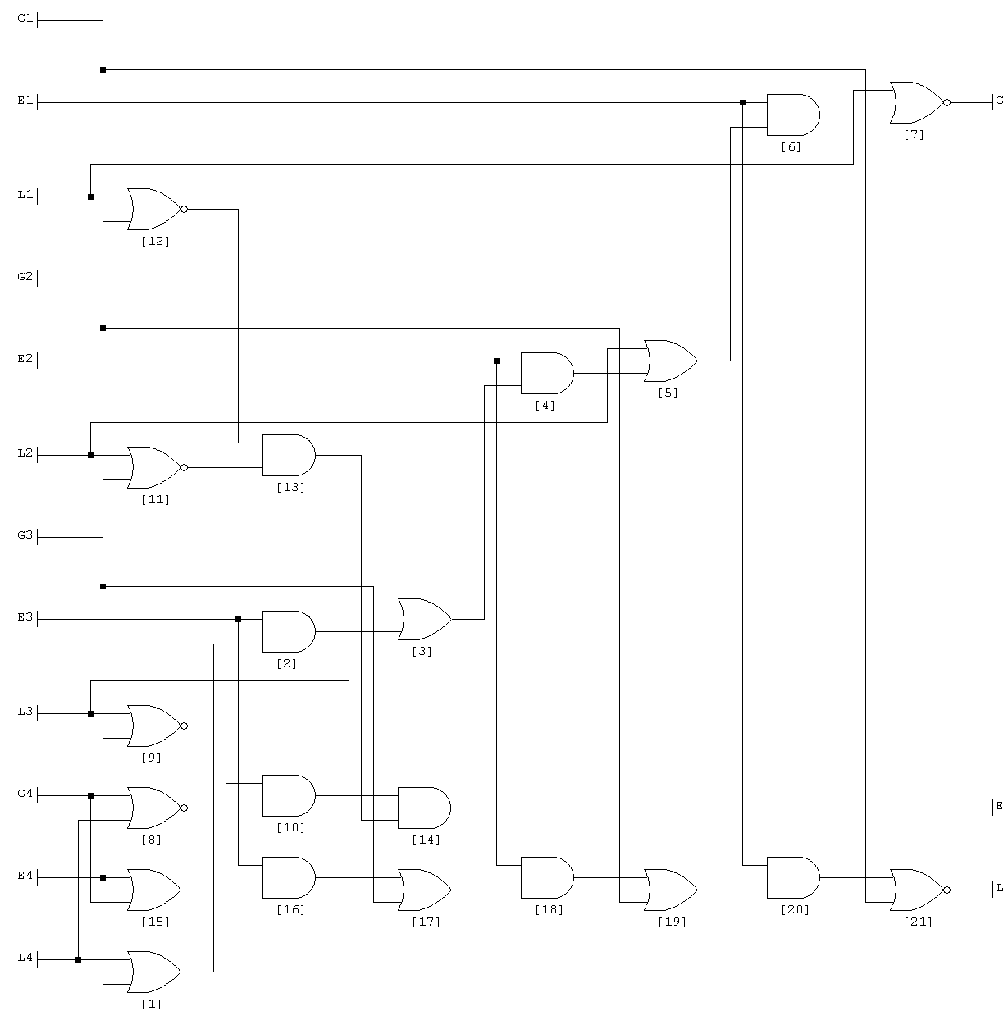
\includegraphics[max width = 0.95\textwidth]{Sol4-3} With L1, G1, E1 as the outputs from the highest four bits, and G4, E4, L4 as the output from the low bits.
                    % This is found via the truth table \lstinputlisting{./chapter04/FigHw/sol4-3.txt}
                    Connect four comparators in a daisy chain with the 16-bit inputs $X$ and $Y$ divided into four 4-bit sub-vectors sent to one of the 4-bit comparators.  The connect
                    the $G_{out}$, $L_{out}$, and $E_{out}$ signals of the more significant comparator to the $G_{in}$, $L_{in}$, and $E_{in}$ of the less significant comparator.
                    Hardwire the $G_{in}$, $L_{in}$, and $E_{in}$ inputs of the most significant comparator (the one with $X(15\ldots12)$ and $Y(15\ldots12)$ as the data inputs)
                    to $0,0,1$ respectively.  Use the  $G_{out}$, $L_{out}$, and $E_{out}$ of the leaqst significant comparator as the  $G_{out}$, $L_{out}$, and $E_{out}$ of the 
                    16-bit comparator.
                }
            \end{onlysolution}

        \item \textbf{ (2 pts.)}Determine the circuitry for the overflow detection
            circuit for a 2's-complement adder subtractor.  See page~\pageref{4-page:Ovf}.

            \begin{onlysolution} \textbf{Solutions} \itshape{
                    $
                    \begin{array} {c||c|c} \\
                        c_{in}  \bs c_{out} & 0 & 1 \\ \hline
                        0    &   & 1 \\ \hline
                        1    & 1 &   \\
                    \end{array}$   \\
                    Thus $ovf = c_{in}' c_{out} + c_{in} c_{out}' =  c_{in} \oplus c_{out} $
                }
            \end{onlysolution}

        \item \textbf{ (10 pts.)}Build a BCD to 7-Segment Display converter using
            Espresso.

            \begin{buildingblock}{BCD to 7-segment}
                \index{bcd to 7-segment}
                \label{page:7seg}
                \begin{tabular}{|l|p{3.5in}|} \hline
                    Nomenclature:  & BCD to 7-segment converter                \\ \hline
                    Data Input:    & 4-bit vector $D=d_3 d_2 d_1 d_0$  \\ \hline
                    Data Output:   & 7-bit vector $Y=y_6 \ldots y_1 y_0$    \\ \hline
                    Control:       & none                                   \\ \hline
                    Status:        & none                                   \\ \hline
                    Behavior:      & The output drives a 7-segment display pattern
                    representing the BCD digit.  \\ \hline
                \end{tabular}
            \end{buildingblock}

            A binary coded digit (BCD) is a 4-bit binary number that is constrained
            to assume the values of 0-9. That is, 1010 ... 1111 are illegal BCD digits.

            A 7-segment display is a box with seven inputs and seven output LED bars.
            Each input is wired to an LED bar that is illuminated when a 1 is applied
            to its input.
            Each of the seven LED segments is numbered according to the pattern shown
            on the left-hand side of Figure~\ref{fig:BCD}.

            \begin{figure}[ht]
                \center{\scalebox{0.7}{\includegraphics{Prob4-5}}}
                \caption{The numbering of the segments in a 7-segment display.
                The patterns of the BCD digits.}
                \label{fig:BCD}
            \end{figure}

            The pattern of LEDs to illuminate for each BCD digit is shown on the
            right-hand side of Figure~\ref{fig:BCD}.  A BCD to 7-segment converter
            has four inputs, $d_3 d_2 d_1 d_0$ and seven outputs $S_7 \ldots S_1$.
            Complete the design using Espresso.  Make sure to include ``Don't cares"
            in the truth table specification.
            \begin{enumerate}
                \item Use Espresso to determine the \SOPmin expression for the outputs
                    $S_7 \ldots S_1$.  Underline product terms that are shared.
                    Submit the Espresso source file.

                    \definecolorseries{BCD7-Table}{hsb}{step}[hsb]{0.35,0.42,1}{.368,0,-0.01} \resetcolorseries[10]{BCD7-Table}
                    \begin{onlysolution} \textbf{Solutions} \itshape{
                            The following is the source file for the BCD to 7-segment converter.\lstinputlisting{./chapter04/FigHw/sol4-5-a.txt}
                            This produces the following gates:\newpage
                            \begin{table}[t]
                                \centering
                                \begin{tabular}{llllll}
                                    s7 =&      \mathcolorbox{BCD7-Table!![0]}{(!d2\&!d1\&!d0)}        & +        \mathcolorbox{BCD7-Table!![2]}{(d1\&!d0)}                & +        \mathcolorbox{BCD7-Table!![6]}{(d2\&!d1\&d0)}         & +        \mathcolorbox{BCD7-Table!![9]}{(!d2\&d1)}                                                                               \\
                                    s6 =&      \mathcolorbox{BCD7-Table!![1]}{(d1\&d0)}               & +        \mathcolorbox{BCD7-Table!![3]}{(!d2\&!d1)}               & +        \mathcolorbox{BCD7-Table!![7]}{(d2\&!d1\&!d0)}        & +        \mathcolorbox{BCD7-Table!![5]}{(d2\&d1)}          & +        \mathcolorbox{BCD7-Table!![6]}{(d2\&!d1\&d0)}              \\
                                    s5 =&      \mathcolorbox{BCD7-Table!![0]}{(!d2\&!d1\&!d0)}        & +        \mathcolorbox{BCD7-Table!![2]}{(d1\&!d0)}                                                                                                                                                                                                                    \\
                                    s4 =&      \mathcolorbox{BCD7-Table!![2]}{(d1\&!d0)}              & +        \mathcolorbox{BCD7-Table!![4]}{(d2\&!d1\&!d0)}           & +        \mathcolorbox{BCD7-Table!![6]}{(d2\&!d1\&d0)}         & +        \mathcolorbox{BCD7-Table!![9]}{(!d2\&d1)}         & +        \mathcolorbox{BCD7-Table!![10]}{(d3)}                       \\
                                    s3 =&      \mathcolorbox{BCD7-Table!![1]}{(d1\&d0)}               & +        \mathcolorbox{BCD7-Table!![3]}{(!d2\&!d1)}               & +        \mathcolorbox{BCD7-Table!![7]}{(d2\&!d1\&!d0)}        & +        \mathcolorbox{BCD7-Table!![9]}{(!d2\&d1)}                                                                               \\
                                    s2 =&      \mathcolorbox{BCD7-Table!![0]}{(!d2\&!d1\&!d0)}        & +        \mathcolorbox{BCD7-Table!![4]}{(d2\&!d1\&!d0)}           & +        \mathcolorbox{BCD7-Table!![5]}{(d2\&d1)}              & +        \mathcolorbox{BCD7-Table!![6]}{(d2\&!d1\&d0)}     & +        \mathcolorbox{BCD7-Table!![10]}{(d3)}                       \\
                                    s1 =&      \mathcolorbox{BCD7-Table!![0]}{(!d2\&!d1\&!d0)}        & +        \mathcolorbox{BCD7-Table!![5]}{(d2\&d1)}                 & +        \mathcolorbox{BCD7-Table!![6]}{(d2\&!d1\&d0)}         & +        \mathcolorbox{BCD7-Table!![9]}{(!d2\&d1)}         & +        \mathcolorbox{BCD7-Table!![10]}{(d3)}               %
                                \end{tabular}
                            \end{table}

                        }
                    \end{onlysolution}

                \item Use Espresso to determine the \POSmin expression for the outputs
                    $S_7 \ldots S_1$.  Underline sum terms that are shared.
                    Submit the Espresso source file
                    \begin{onlysolution} \textbf{Solutions} \itshape {
                        If we run the same file as part a with the -epos flag, it will preform a minimization on the off-set of our functions. If we take this output and invert it, we will have our \POSmin expression.} \\
                        \begin{table}[h]
                            \centering
                            \begin{tabular}{*{7}{l}}
                                s7 =& \mathcolorbox{BCD7-Table!![0]}{(d3 + d2 + d1 + !d0)}  &$\&$ \mathcolorbox{BCD7-Table!![3]}{(!d2 + d1 + d0)}       &$\&$ \mathcolorbox{BCD7-Table!![5]}{(!d3 + !d0)}       &$\&$ \mathcolorbox{BCD7-Table!![4]}{(!d2 + !d1 + !d0)} & ~ & ~ \\
                                s6 =& \mathcolorbox{BCD7-Table!![1]}{(d2 + !d1 + d0)}       & ~                     & ~ & ~ & ~ & ~ \\
                                s5 =& \mathcolorbox{BCD7-Table!![2]}{(!d2 + d1 + !d0)}      &$\&$ \mathcolorbox{BCD7-Table!![0]}{(d3 + d2 + d1 + !d0)}  &$\&$ \mathcolorbox{BCD7-Table!![6]}{(d2 + !d1 + !d0)}  &$\&$ \mathcolorbox{BCD7-Table!![3]}{(!d2 + d1 + d0)}   &$\&$ \mathcolorbox{BCD7-Table!![5]}{(!d3 + !d0)} &$\&$ \mathcolorbox{BCD7-Table!![4]}{(!d2 + !d1 + !d0)} \\
                                s4 =& (d3 + d2 + d1)        &$\&$ \mathcolorbox{BCD7-Table!![4]}{(!d2 + !d1 + !d0)}     & ~ & ~ & ~ & ~ \\
                                s3 =& (!d2 + !d1 + d0)      &$\&$ \mathcolorbox{BCD7-Table!![2]}{(!d2 + d1 + !d0)}      & ~ & ~ & ~ & ~ \\
                                s2 =& \mathcolorbox{BCD7-Table!![1]}{(d2 + !d1 + d0)}       &$\&$ \mathcolorbox{BCD7-Table!![0]}{(d3 + d2 + d1 + !d0)}  &$\&$ \mathcolorbox{BCD7-Table!![6]}{(d2 + !d1 + !d0)}  & ~ & ~ & ~ \\
                                s1 =& \mathcolorbox{BCD7-Table!![0]}{(d3 + d2 + d1 + !d0)}  &$\&$ \mathcolorbox{BCD7-Table!![3]}{(!d2 + d1 + d0)}       & ~ & ~ & ~ & ~ \\
                            \end{tabular}
                        \end{table}
%% \begin{verbatim}
%% # BCD to 7-segment display
%% #
%% .i 4
%% .o 7
%% .ilb b3 b2 b1 b0
%% .ob s7 s6 s5 s4 s3 s2 s1
%% #.phase 0000000
%% .p 9
%% 000- 0001000
%% -110 0000100
%% -010 0100010
%% -101 0010100
%% 0001 1010011
%% -011 0010010
%% -100 1010001
%% 1--1 1010000
%% -111 1011000
%% .e
%% \end{verbatim}
                    \end{onlysolution}
            \end{enumerate}

            \filbreak % Strongly suggest page break
        \item \textbf{(10 pts.)} Build a box which has one 4-bit input called A and
            one 4-bit output called T. The output T is the 2's-complement value
            of the input A.  Use the bit slice paradigm to solve this
            problem.  That is, create a building block for one bit of the problem
            then string four of them together to solve the problem.
            For the problem at hand this can be done as follows:
            \begin{enumerate}
                \item Start at the LSB of A.
                \item If this is the first, least significant, 1, flip all bits
                    to the left.
                \item If this is not the first 1, leave the bit alone.
                \item Move one bit to the left.
                \item Goto Step b.
            \end{enumerate}
            A bit-slice should communicate whether there has been a 1 to the right,
            to the more significant bit.  Submit:
            \begin{itemize}
                \item How the above "algorithm" behaves when presented with
                    the inputs A=1100
                    \begin{onlysolution}
                        \textit{\color{blue}
                            \begin{enumerate}
                                \item Move one bit to the left
                                \item Move one bit to the left
                                \item Flip. Move one bit to the left
                                \item Flip. Move one bit to the left
                            \end{enumerate}}
                    \end{onlysolution}
                \item The truth table for one bit slice
                    \begin{onlysolution}

                    \end{onlysolution}
                \item \SOPmin expression and circuit diagram for a bit slice.
                    \begin{onlysolution}

                    \end{onlysolution}
                \item The organization of four bit slices to solve the problem
                    \begin{onlysolution}

                    \end{onlysolution}
            \end{itemize}

            \begin{onlysolution} \textbf{Solutions} \itshape{
                    The key to the begin solution  is to figure out the structure
                    of the begin solution  and then give meaning to the signals involved.
                    The problem will be sliced into four bit-slices; each handled
                    but its own complement box.  Thus, there will be four complement
                    box in the begin solution.  Each box will have 2 inputs, one being
                    a bit of A and the other being a "carry in" from the less
                    significant less, immediately to the right.  Each box
                    will have two bits of output, a bit of T and a "carry out".
                    The carry bits (both into and out of a box will convey
                    information regarding the rightmost 1 in the number A.)

                    If the carry in is equal 1 then there is a one to the right.
                    If the carry in is equal 0 then there is not a one to the right.
                    The truth table for a box is then

                    \begin{table}[h]
                        \begin{tabular}{l|l||l|l|l}
                            $A$ & $c_{in}$  & $T$ & $c_{out}$ & comment \\ \hline
                            0   & 0       &   0 & 0          & There is no 1 to the right \\ \hline
                            0   & 1       &   1 & 1          & There is a 1 to the right, flip A \\ \hline
                            1   & 0       &   1 & 1          & There is is no 1 to the right, but we've
                            created one \\ \hline
                            1   & 1       &   0 & 1          & There is a 1 to the right, flip A \\
                        \end{tabular}
                    \end{table}

                    From this it follows that: \\
                    $T=A'c_{in} + A c_{in}'=A \oplus c_{in}$ \\
                    $c_{out} = A + c_{in}$
                }
            \end{onlysolution}
        \item \textbf{(4 pts.)} Build a 7:128 decoder using a minimum number of
            4:16, 2:4 and 1:2 decoders. Describe the wiring of the select lines.

            \begin{onlysolution} \textbf{Solutions}
                \begin{figure}[h]
                    \centering
                    \includegraphics[height=0.8\textheight]{Sol4-7}
                    \caption{A 7:128 decoder built from 4:16, 2:4 and 1:2 decoders.}
                    \label{fig:bighwdec}
                \end{figure}
                \filbreak
            \end{onlysolution}
        \item \textbf{(4 pts. each)} Design a circuit with two 8-bit inputs $X,Y$, an
            8-bit output $Z$ and a 1-bit input $sel$.  Construct a circuit that yields the
            correct value of $Z$ using only the basic building blocks presented in this
            chapter; do NOT show the internal organization of these building blocks.  If
            a mux is used, denote which input is the $y_0$ and which is $y_1$.
            If a comparator is used denote which input is $X$ and which is $Y$.
            Do not use any AND or OR gates; it will tempting in the later problems.
            \begin{enumerate}
                \item \verb^ if (sel==0) then Z = X else Z = Y ^

                    \begin{onlysolution} \textbf{Solutions} \itshape{
                            \includegraphics{Sol4-8a}
                        }
                    \end{onlysolution}

                \item \verb^ if (sel==0) then Z = X+Y else Z = Y ^

                    \begin{onlysolution} \textbf{Solutions} \itshape{
                            \includegraphics{Sol4-8b}
                        }
                    \end{onlysolution}

                \item \verb^ if (sel==0) then Z = X+Y else Z = X-Y ^

                    \begin{onlysolution} \textbf{Solutions} \itshape{
                            \includegraphics{Sol4-8c}
                        }
                    \end{onlysolution}

                \item \verb^ if (X==0) then Z = X else Z = Y ^

                    \begin{onlysolution} \textbf{Solutions} \itshape{
                            \includegraphics{Sol4-8d}
                        }
                    \end{onlysolution}

                \item \verb^ if (X==Y) then Z = X-Y else Z = Y ^

                    \begin{onlysolution} \textbf{Solutions} \itshape{
                            \includegraphics{Sol4-8e}
                        }
                    \end{onlysolution}

                \item \verb^ if (X==Y) then Z = X+Y else Z = X-Y ^

                    \begin{onlysolution} \textbf{Solutions} \itshape{
                            \includegraphics{Sol4-8f}
                        }
                    \end{onlysolution}

                \item \verb^ if (X < Y) then Z = X else Z = Y ^

                    \begin{onlysolution} \textbf{Solutions} \itshape{
                            \includegraphics{Sol4-8g}
                        }
                    \end{onlysolution}

                \item \verb^ if (X <= Y) then Z = X else Z = Y ^

                    \begin{onlysolution} \textbf{Solutions} \itshape{
                            \includegraphics{Sol4-8h}
                        }
                    \end{onlysolution}

                \item \verb^ if (X > Y) then Z = X else Z = Y ^

                    \begin{onlysolution} \textbf{Solutions} \itshape{
                            \includegraphics{Sol4-8i}
                        }
                    \end{onlysolution}

                \item \verb^ if (X > Y) then Z = X+X else Z = Y+Y ^

                    \begin{onlysolution} \textbf{Solutions} \itshape{
                            \includegraphics{Sol4-8j}
                        }
                    \end{onlysolution}

            \end{enumerate}

        \item \textbf{ (10 pts.)} Build a 4-bit priority encoder.

            \begin{buildingblock}{Priority Encoder}
                \index{priority encoder}
                \begin{tabular}{|l|p{3.5in}|} \hline
                    Nomenclature:  & N-bit priority encoder                \\ \hline
                    Data Input:    & N-bit vectored  $D=d_{N-1} \ldots d_1 d_0$  \\ \hline
                    Data Output:   & $\log_2(N)$-bit vector $Y=y_{log_2(N)} \ldots y_1 y_0$    \\ \hline
                    Control:       & none                    \\ \hline
                    Status:        & none                                   \\ \hline
                    Behavior:      & $F = i$ where $i$ is the highest indexed input
                    which equals 1.  When all inputs equal
                    0, the output is a ``don't care".  \\ \hline
                \end{tabular}
                \label{page:prior}
            \end{buildingblock}

            The idea is for the outputs to represent (in binary code) the highest
            input index which equals 1.  For example, a 4-bit priority encoder
            with input $D=1010$ has inputs $d_3=1$ and $d_0=1$.  Of these two
            inputs, the index of $d_3$ is greater than the index of $d_0$ so the
            output, $F$ is equal to 3, or in binary $11$.  If the input were
            $D=0111$ then $F=10$.

            \begin{enumerate}
                \item Write down the truth table for a 4-bit priority encoder.  Hint,
                    the truth table could be structured so that it contains only five rows
                    by using ``don't cares" on the inputs.

                    \begin{onlysolution} \textbf{Solutions} \itshape{
                            \begin{tabular}{l|l|l|l||l|l}
                                $d_3$ & $d_2$ & $d_1$ & $d_0$ & $f_1$ & $F_0$ \\ \hline
                                0  &    0  &    0  &    0  &    x  &    x  \\ \hline
                                0  &    0  &    0  &    1  &    0  &    0  \\ \hline
                                0  &    0  &    1  &    x  &    0  &    1  \\ \hline
                                0  &    1  &    x  &    x  &    1  &    0  \\ \hline
                                1  &    x  &    x  &    x  &    1  &    1  \\
                            \end{tabular}
                        }
                    \end{onlysolution}

                \item An \SOPmin realization of the circuit.
                    \begin{onlysolution} \textbf{Solutions} \itshape{
                            $f_1 = d_3 + d_2$ \\
                            $f_0 = d_3 + d_2'd_1$
                        }
                    \end{onlysolution}
            \end{enumerate}

        \item \textbf{ (10 pts.)} Build a 4-bit saturation adder.  A
            saturation adder performs normal 4-bit addition when the
            resulting sum is less than 15.  If the sum is
            greater than 15, the saturation adders outputs 15.  The
            following table summarizes.

            \begin{buildingblock}{Saturation Adder}
                \index{saturation adder}
                \label{page:saturation}
                \begin{tabular}{|l|p{3.5in}|} \hline
                    Nomenclature:  & 4-bit saturation adder                \\ \hline
                    Data Input:    & 2, 4-bit vectors \verb+A, B+  \\ \hline
                    Data Output:   & 4-bit vector \verb+sum+    \\ \hline
                    Control:       & none                                   \\ \hline
                    Status:        & none                                   \\ \hline
                    Behavior:      &
                \begin{verbatim}
                if (A+B > 15) sum = 15
                else sum = A+B
                \end{verbatim}
                    \\ \hline
                \end{tabular}
            \end{buildingblock}

            Submit a schematic showing the basic building blocks, their
            data status, and control interconnections.  Show any truth
            tables used to build glue logic.

            \begin{onlysolution} \textbf{Solutions} \itshape{
                    All we need to do is to determine when the sum is greater then
                    15 and output 15 when it is.  The comparator/mux combo mentioned
                    several times in the chapter should do the trick.

                    \includegraphics{Sol4-10}

                }
            \end{onlysolution}

        \item \textbf{ (10 pts.)} Build a mod-6 adder.  The mod-6 adder
            takes as input two 3-bit (mod 6) numbers and adds them together
            modulus 6.

            \index{modular arithmetic}
            \label{page:mod}
            Modular arithmetic only operates with a limited portion of the
            integers.  The range of numbers is $\{0,1,2, \ldots ,m-1\}$ where
            $m$ is called the \textit{ modulus}; note there are $m$ different
            integers because counting started at 0.  For example, when working
            in mod-6 arithmetic use the integers $\{0,1,2,3,4,5\}$.
            To solve any addition problem in modular arithmetic, it is only
            necessary to perform regular addition with the special rule that
            the addition process rolls over from the largest number, $m-1$ to 0
            when the result is larger than $m-1$.  For
            example, in mod-6 arithmetic $(5+1) \mod 6 = 0$.  The statement
            ``$\mod 6$" is always included in the addition problem to indicate
            to the reader that mod-6 arithmetic is being performed.  Here
            are a few more examples to help

            \begin{tabular}{l}
                $2+3~\mod 6 = 5$ \\
                $3+3~\mod 6 = 0$ \\
                $4+3~\mod 6 = 1$ \\
                $5+5~\mod 6 = 4$
            \end{tabular}

            \index{modular adder}
            \label{page:modadder}
            \begin{tabular}{|l|p{3.5in}|} \hline
                Nomenclature:  & 3-bit mod 6 adder                \\ \hline
                Data Input:    & two, 3-bit (mod-6) vectors \verb+A, B+  \\ \hline
                Data Output:   & 3-bit (mod-6) vector \verb+sum+    \\ \hline
                Control:       & none                                   \\ \hline
                Status:        & none                                   \\ \hline
                Behavior:      &
                \begin{verbatim}
                sum = A+B mod 6
                \end{verbatim}
                \\ \hline
            \end{tabular}

            Submit a schematic showing the basic building blocks, their
            data status, and control interconnections.  Show any truth
            tables used to build glue logic.  Be careful that the word
            size of the result is handled correctly.

            \begin{onlysolution} \textbf{Solutions} \itshape{
                    Since the inputs are mod 6 numbers then the inputs can be in the
                    range [0-5].  Adding two such values will yield a value in the
                    range [0-10].  Hence a simple adjustment of the sum when its larger
                    that 5 is required.

                    \includegraphics{Sol4-11}

                }
            \end{onlysolution}

        \item \textbf{ (1pt. each)}Convert the following to 2's-complement
            assuming a word size of eight bits.
            \begin{enumerate}
                \item -35

                    \begin{onlysolution} \textbf{Solutions} \itshape{
                            $35 = 32+2+1 = 100011 = 00100011$, thus $-35=11011101$
                        }
                    \end{onlysolution}

                \item  -128

                    \begin{onlysolution} \textbf{Solutions} \itshape{
                            This is a special case, see page 10 for more information.
                            $-128 = 10000000$
                        }
                    \end{onlysolution}

                \item  67

                    \begin{onlysolution} \textbf{Solutions} \itshape{
                            $67=64+2+1 = 100 0011 = 0100 0011$
                        }
                    \end{onlysolution}

                \item  128

                    \begin{onlysolution} \textbf{Solutions} \itshape{
                            There are not enough bits to represent this positive number; hence
                            the 8-bit representation does not exist.
                        }
                    \end{onlysolution}

            \end{enumerate}
            \filbreak
        \item \textbf{ (1 pt. each)} Perform the following operations for the given
            2's-complement numbers. Assume a word size of eight bits
            in all cases. Indicate where overflow occurs. If there is no overflow,
            convert the result to decimal.
            \begin{enumerate}

                \item 01011101 + 00110111

                    \begin{onlysolution} \textbf{Solutions}
                        \begin{align*}
                            {\color{gray}
                            1111\,111\0 }&\\[-1.5ex]
                            0101\,1101&\\
                            +\:0011\,0111&\\[-2ex]
                            \rule{12ex}{1pt}\hspace{-1ex}&\\[-1ex]
                            1001\,0100&\quad  overflow
                        \end{align*}
                    \end{onlysolution}

                \item 11101011 + 11110001

                    \begin{onlysolution} \textbf{Solutions}
                        \begin{align*}
                            {\color{gray}
                            111\0\0\911\0 }&\\[-1.5ex]
                            1110\,1011&\\
                            +\:1111\,0001&\\[-2ex]
                            \rule{12ex}{1pt}\hspace{-1ex}&\\[-1ex]
                            1101\,1100&
                        \end{align*}
                    \end{onlysolution}

                \item 01011101 + 10101011

                    \begin{onlysolution} \textbf{Solutions}
                        \begin{align*}
                            {\color{gray}
                            11111\,111\0}&\\[-1.5ex]
                            0101\,1101&\\
                            +\:1010\,1011&\\[-2ex]
                            \rule{12ex}{1pt}\hspace{-1ex}&\\[-1ex]
                            0000\,1000&
                        \end{align*}
                    \end{onlysolution}

                \item 10111011 - 11110001

                    \begin{onlysolution} \textbf{Solutions}
                        \begin{alignat*}{3}
                            &&{\color{gray}
                            1\,111\0 }\\[-1.5ex]
                            1110\,1011&   &1110\,1011\\
                            -\:1111\,0001&&+\:0000\,1111\\[-2ex]
                            \rule{12ex}{1pt}\hspace{-1ex}&\ \raisebox{3.5ex}[0pt][0pt]{$\xLongrightarrow{\phantom{80em}}$}\ &\rule{12ex}{1pt}\hspace{-1ex}\\[-1ex]
                            & &1101\,1010
                        \end{alignat*}
                    \end{onlysolution}

                \item 01011101 - 00110111

                    \begin{onlysolution} \textbf{Solutions}
                        \begin{alignat*}{3}
                            &&{\color{gray}
                            11\011\9\01\0 }\\[-1.5ex]
                            0101\,1101&&   0101\,1101\\
                            -\:0011\,0111&&+\:1100\,1001\\[-2ex]
                            \rule{12ex}{1pt}\hspace{-1ex}&\ \raisebox{3.5ex}[0pt][0pt]{$\xLongrightarrow{\phantom{80em}}$}\ &\rule{12ex}{1pt}\hspace{-1ex}\\[-1ex]
                            &&   0010\,0110
                        \end{alignat*}
                    \end{onlysolution}

                \item 01011101 - 10101111

                    \begin{onlysolution} \textbf{Solutions}
                        \begin{alignat*}{3}
                            &&{\color{gray}
                            \1 1\9\0\01\0 }\\[-1.5ex]
                            0101\,1101&&   0101\,1101\\
                            -\:1010\,1111&&+\:0101\,0001\\[-2ex]
                            \rule{12ex}{1pt}\hspace{-1ex}&\ \raisebox{3.5ex}[0pt][0pt]{$\xLongrightarrow{\phantom{80em}}$}\ &\rule{12ex}{1pt}\hspace{-1ex}\\[-1ex]
                            &&1010\,1110&\ \textit{overflow}
                        \end{alignat*}
                    \end{onlysolution}

            \end{enumerate}

        \item \textbf{ (10 pts.)}
            \label{page:flipbox}
            Build a flip box.  A flip box is defined by the following input,
            output, and behavior definition.

            \begin{tabular}{|l|p{3.5in}|} \hline
                Nomenclature:  & 8-bit flip box.                    \\ \hline
                Data Input:    & 8-bit $D=d_7 \ldots d_0$          \\ \hline
                Data Output:   & 8-bit $F=f_7 \ldots f_0$          \\ \hline
                Control:       & 3-bit $S=s_2 s_1 s_0$            \\ \hline
                Status:        & none                                   \\ \hline
                Behavior:      & The output is the same as the input except for
                one bit which is inverted.  The index of the inverted
                bit is given by $S$. \\ \hline
            \end{tabular}

            The flip box takes the 8-bit data input, flips a single bit identified
            by $S$, then sends the new 8-bit value to the output.
            For example, if $D=11110000$ and $S=010$ then
            $F=11110100$.  If $D=11110000$ and $S=101$ then $F=11010000$.  The solution
            should rely heavily on the basic building blocks.

            \begin{onlysolution} \textbf{Solutions} \itshape{
                    Arrange 8, 2:1 muxes with $d_i$ and $d_i'$ going into the data inputs.
                    Run the select into a 3:8 decoder and route the data outputs to the
                    individual selects of the 2:1 muxes.
                }
            \end{onlysolution}

        \item \textbf{(10 pts.)}
            \label{page:IsScan}
            Build a box which recognizes some keyboard scancode.  When a key is
            pressed on a keyboard, the keyboard transmits (among other things)
            an 8-bit scancode of the pressed key.  Each key has its own scancode
            listed in Table~\ref{table:scancodes}.  The relationship between the
            keys and their scancode is not based on ASCII.

            \begin{table}[h]
                \begin{tabular}{|l|l||l|l||l|l||l|l|} \hline
                    Key & scancode & Key & scancode & Key & scancode & Key & scancode \\ \hline \hline
                    0 & $45_{16}$ & 1 & $16_{16}$ & 2 & $1E_{16}$ & 3 & $26_{16}$ \\ \hline
                    4 & $25_{16}$ & 5 & $2E_{16}$ & 6 & $36_{16}$ & 7 & $3D_{16}$ \\ \hline
                    8 & $3E_{16}$ & 9 & $46_{16}$ & A & $1C_{16}$ & B & $32_{16}$ \\ \hline
                    C & $21_{16}$ & D & $23_{16}$ & E & $24_{16}$ & F & $2B_{16}$ \\ \hline
                    P & $4D_{16}$ & L & $4B_{16}$ & M & $3A_{16}$ & I & $43_{16}$ \\ \hline
                \end{tabular}
                \caption{IBM 6450225 Keyboard scancodes.}%\footnote{it is based on an \href{https://www.seasip.info/VintagePC/ibm_6450225.html}{IBM 6450225 Keyboard}}
                \label{table:scancodes}
            \end{table}
            \label{page:scanclass}
            \begin{tabular}{|l|p{3.5in}|} \hline
                Nomenclature:  & scancode classifier                   \\ \hline
                Data Input:    & 8-bit $D=d_7 \ldots d_0$          \\ \hline
                Data Output:   & IsP, IsL, IsM, IsI, IsS \\ \hline
                Control:       & none             \\ \hline
                Status:        & none                                   \\ \hline
                Behavior:      & IsP =1 when $D$ is the scan code for the letter ``P".
                IsL =1 when $D$ is the scan code for the letter ``L".
                IsM =1 when $D$ is the scan code for the letter ``M".
                IsI =1 when $D$ is the scan code for the letter ``I".\\ \hline
                %IsS =1 when $D$ is the scan code for the letter ``S".{\color{blue}($1B_{16}$)}  \\ \hline
            \end{tabular}\\
            \begin{onlysolution} \textbf{Solution:}
                \textit{\color{blue} We would simply need 4 comparators testing if the incoming scan code is equal to $4D_{16}$ (IsP), $4B_{16}$ (IsL), $3A_{16}$ (IsM), or $43_{16}$ (IsI).}\\
                \includegraphics[max width = 0.8\textwidth]{sol4-15}

            \end{onlysolution}
            \filbreak
        \item \textbf{(10 pts.)}
            \label{page:ScanDecode}
            Build a box which converts an 8-bit scancode for a hexadecimal digit into a 4-bit hexadecimal values.

            \label{page:scanconv}
            \begin{tabular}{|l|p{3.5in}|} \hline
                Nomenclature:  & scancode classifier                   \\ \hline
                Data Input:    & 8-bit $D=d_7 \ldots d_0$          \\ \hline
                Data Output:   & 4-bit $H=h_3h_2h_1h_0$ \\ \hline
                Control:       & none             \\ \hline
                Status:        & none                                   \\ \hline
                Behavior:      & Converts the scancode $D$, representing a the
                key of a hexadecimal character, into its 4-bit
                value $H$.
                \\ \hline
            \end{tabular}

            For example, if $D=25_{16}$, the scancode for the "4" key, then the converter
            should output $H=0100_2$.  Assume that the inputs are always
            legal hexadecimal scancodes.
            \begin{onlysolution}
                {\color{blue}

                    \begin{table}[!ht]
                        \centering
                        {\color{blue}
                            \lstinputlisting{./chapter04/FigHw/sol4-16.txt   }
                            \lstinputlisting{./chapter04/FigHw/sol4-16-ex.txt}
                        }
                \end{table}}
            \end{onlysolution}
    \end{enumerate}


%\setcounter{chapter}{5}
%\setcounter{section}{-1}
\chapter{Sequential Circuits}
\section{Exercises}
\label{section:sequentialCircuitsExercises}
\graphicspath{ {./chapter05/FigHw} }

\begin{enumerate}

    \item \textbf{ (8 pts.)}Determine the state table for the circuit in Figure~\ref{fig:sequentialCirNANDs}.
        \begin{figure}[ht]
            \center{\includegraphics{Prob5-1}}
            \caption{}
            \label{fig:sequentialCirNANDs}
        \end{figure}

        \begin{onlysolution}  \textbf{Solution} \itshape{
                The analysis of the cross-coupled NANDs show in Figure~\ref{fig:sequentialCirNANDs} is
                almost exactly the same as that for the cross coupled NORs.  Start with
                the truth table for an NAND gate:

                \begin{tabular}{l|l||l}
                    a & b & (ab)' \\ \hline
                    0 & 0 & 1 \\ \hline
                    0 & 1 & 1 \\ \hline
                    1 & 0 & 1 \\ \hline
                    1 & 1 & 0 \\
                \end{tabular}

                Observe that the output is 1 whenever
                either input is 0.  Now onto the state table for the cross coupled NANDs:

                \begin{tabular}{l|l||l|l}
                    A & B & $F^+$ & $G^+$ \\ \hline
                    0 & 0 & 1 & 1 \\ \hline
                    0 & 1 & 1 & 0 \\ \hline
                    1 & 0 & 0 & 1 \\ \hline
                    1 & 1 & F & G \\
                \end{tabular}

                For the cross coupled NANDs the output holds when the input $A,B=1,1$ occurs.
                In fact if you compare this table to that of the cross coupled NORs, you will
                notice that $A,B = S',R'$ and $F,G = Q,Q'$.
            }
        \end{onlysolution}

    \item \textbf{ (8 pts.)} Determine the state table for the circuit
        in Figure~\ref{fig:sequentialCirDLatch}.  Which basic memory element does it act
        like?  Hint, one of the inputs is acting like a clock.  Additional
        hint, in order to simplify the analysis, replace a portion of the
        circuit with a component from this chapter.
        \begin{figure}[ht]
            \center{\includegraphics{Prob5-2}}
            \caption{}
            \label{fig:sequentialCirDLatch}
        \end{figure}

        \begin{onlysolution}  \textbf{Solution} \itshape{
                The main idea in this problem is to simplify the cross coupled NOR gates into
                an SR latch.  Then use the state table for the SR latch.  This substitution
                will simplify the analysis of this circuit.  Since the lower NOR gate is denoted
                $A$, call the lower input of the SR latch $R$ and the upper input $S$
                (see Figure 5.6).

                This yields the following truth table:

                \begin{tabular}{l|l|l|l|l||l}
                    A & B & S & R & comment & $Q^+$ \\ \hline
                    0 & 0 & 0 & 0 & Hold    & $Q$   \\ \hline
                    0 & 1 & 0 & 0 & Hold    & $Q$   \\ \hline
                    1 & 0 & 0 & 1 & Reset   & 0     \\ \hline
                    1 & 1 & 1 & 0 & Set     & 1     \\
                \end{tabular}

                It is behaving exactly like a D clocked latch, where $A=clk$ and $B=D$.
            }
        \end{onlysolution}

    \item \textbf{ (8 pts.)} Complete the timing diagram for the circuit
        shown in Figure~\ref{fig:sequentialCirDMS}.  Which basic memory element
        does this circuit act like?

        \ifshowanswers \textbf{Solution} \fi

        \begin{figure}[ht]
            \label{fig:sequentialCirnand}
            \center{\scalebox{0.8}{
                    \ifshowanswers \includegraphics{sol5-3}
                    \else \includegraphics{prob5-3}\fi
            }}
            \caption{A 2-stage sequential circuit.}
            \label{fig:sequentialCirDMS}
        \end{figure}
        \ifshowanswers \textit{\color{blue} This circuit is acting like a Negative Edge Triggered D Flip Flop.}\fi
        \filbreak %h! won't prevent content beneath it from filling, so we need to give it some help with keeping them together
    \item \textbf{ (15 pts.)} Complete the timing diagram for the basic memory
        elements in Figure~\ref{fig:sequentialCirExTim}.  The clock cycle is 20 ns. When
        necessary, assume that $Q$ is initialized to 0 and the output settles to
        0 after a period of rapid toggling. \needspace{4.78in} % tell it that we really do want it to keep this question next to the figure
        \ifshowanswers \textbf{Solution} \fi
        \begin{figure}[ht]
            \center{\scalebox{0.5}{
                    \ifshowanswers \includegraphics{sol5-4} \else \includegraphics{prob5-4} \fi
            }}
            \caption{A variety of basic memory elements and the signals applied to them.}
            \label{fig:sequentialCirExTim}
        \end{figure}
    \item \textbf{ (15 pts.)} Complete the timing diagram for the basic memory elements in
        Figure~\ref{fig:sequentialCirExTim2}.  The clock cycle is 20 ns. When necessary,
        assume that Q is initialized to 0 and the output settles to 0 after
        a period of rapid toggling.\par
        \ifshowanswers \textbf{Solution} \fi
        \begin{figure}[ht]
            \center{\scalebox{0.5}{
                    \ifshowanswers \includegraphics{sol5-5} \else \includegraphics{prob5-5} \fi
            }}
            \caption{}
            \label{fig:sequentialCirExTim2}
        \end{figure}
        \filbreak
    \item \textbf{ (4 pts.)} Consider the furnace
        controller discussed at the beginning of this chapter.  Determine
        which state the controller should transition into when in a particular state
        and given a particular combination of inputs.
        Fill in the eight entries in the following table with the next state
        the system should move into.  The next state should be either ON if the
        system should transition (or remain in) the ON state, OFF if the system
        should transition (or remain in) the OFF state, or X if the input
        combination is meaningless.
        \begin{onlyproblem} % Compress the problem version as it can be trivially recreated
            \center{
                \begin{tabular}{c||c|c|c|c}CurrentState$\bs~T_{hi}T_{low}$&00&01&11&10\\\hline\hline ON&&&&\\ \hline OFF&&&&\\
            \end{tabular}}
        \end{onlyproblem}
        \begin{onlysolution}
            \center{
                \begin{tabular}{c||c|c|c|c}
                    Current State $\bs T_{hi} T_{low}$ & 00  & 01 & 11 & 10  \\ \hline \hline
                    ON                                 & ON  & ON & X  & OFF \\ \hline
                    OFF                                & OFF & ON & X  & OFF \\
            \end{tabular}}
        \end{onlysolution}

    \item \textbf{ (8 pts.)} Derive the next state equations for each
        type (D, T, SR, and JK) of basic memory element.  The next state equation
        is a symbolic equation describing the next state ($Q^+$)
        as a function of the inputs (D,T,SR, or JK) and state ($Q$).
        In order to determine the next state equations for a
        a JK memory element, build a 3-variable Kmap with
        $Q$, $J$, and $K$ as the inputs.  The entries in the Kmap should
        be $Q^+$.  Solving this Kmap will yield the next state equation.
        Show all work for full credit.
        \begin{onlysolution}
            \begin{figure}[ht]
                \center{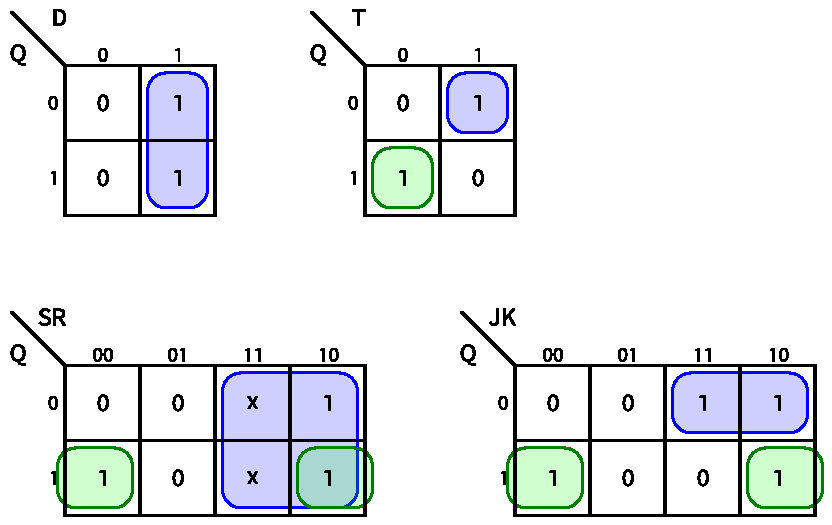
\includegraphics{sol5-7-DC}}
                \caption{}
            \end{figure}
            {\color{blue}\addtolength{\tabcolsep}{-0.4em}
                \begin{tabular}{*{3}{l}}
                    $Q^+_D   $   &$= D         $& ~                              \\[0.1em]
                    $Q^+_T   $   &$= Q'T + QT' $&$= (Q+T)(Q'+T') = Q\oplus T$    \\[0.1em]
                    $Q^+_{SR}$   &$= SR'+R'Q   $&$= (Q+S)(R')   $                \\[0.1em]
                    $Q^+_{JK}$   &$= Q'J + QK' $&$= (Q+J)(Q'+K')$
            \end{tabular}}
        \end{onlysolution}
    \item \textbf{ (16 pts.)} Derive the transition list for each
        type (D, T, SR, and JK) of basic memory element.  A transition
        list describes the input(s) necessary to elicit a particular
        change in state.  For example, imagine that a D flip flop output
        is currently in the 0 state and it needs to transition to
        the 1 state after the clock edge.  In other words, $Q=0$ and
        $Q^+ = 1$.  What input would have to be provided on the
        $D$ input to make this happen?  Clearly, $D=1$.  This entry
        is filled in Table~\ref{table:tl}.

        Hint, the Kmaps used to determine the next state equations
        will help in visualizing all the conditions which elicit
        a particular change of input.  Complete the transition list
        for all four memory types.  For full credit, show how the
        entries in the transition list are determined.

        \begin{table}[ht]
            \center{
                \begin{onlyproblem}
                    \begin{tabular}{cccc}
                        \begin{tabular}{c||c}$Q\rightarrow~Q^+$&D\\\hline\hline$0\rightarrow0$&\\\hline$0\rightarrow1$&1\\\hline$1\rightarrow0$&\\\hline$1\rightarrow1$&\\
                        \end{tabular}&
                        \begin{tabular}{c||c}$Q\rightarrow~Q^+$&T\\\hline\hline$0\rightarrow0$&\\\hline$0\rightarrow1$&\\\hline$1\rightarrow0$&\\\hline$1\rightarrow1$&\\
                        \end{tabular}&
                        \begin{tabular}{c||c|c}$Q\rightarrow~Q^+$&S&R\\\hline\hline$0\rightarrow0$&&\\\hline$0\rightarrow1$&&\\\hline$1\rightarrow0$&&\\\hline$1\rightarrow1$&&\\
                        \end{tabular}&
                        \begin{tabular}{c||c|c}$Q\rightarrow~Q^+$&J&K\\\hline\hline$0\rightarrow0$&&\\\hline$0\rightarrow1$&&\\\hline$1\rightarrow0$&&\\\hline$1\rightarrow1$&&\\
                        \end{tabular}\\
                    \end{tabular}
                \end{onlyproblem}
                \begin{onlysolution}{\color{blue}
                        \begin{tabular}{cccc}

                            \begin{tabular}{c||c}
                                $Q \rightarrow Q^+$ &   D           \\ \hline \hline
                                $0 \rightarrow 0$   &   0           \\ \hline
                                $0 \rightarrow 1$   &   1           \\ \hline
                                $1 \rightarrow 0$   &   0           \\ \hline
                                $1 \rightarrow 1$   &   1           \\
                            \end{tabular}

                            &

                            \begin{tabular}{c||c}
                                $Q \rightarrow Q^+$ &   T           \\ \hline \hline
                                $0 \rightarrow 0$   &   0           \\ \hline
                                $0 \rightarrow 1$   &   1           \\ \hline
                                $1 \rightarrow 0$   &   1           \\ \hline
                                $1 \rightarrow 1$   &   0           \\
                            \end{tabular}

                            &

                            \begin{tabular}{c||c|c}
                                $Q \rightarrow Q^+$ &   S   &   R   \\ \hline \hline
                                $0 \rightarrow 0$   &   0   &   0,1 \\ \hline
                                $0 \rightarrow 1$   &   1   &   0   \\ \hline
                                $1 \rightarrow 0$   &   0   &   1   \\ \hline
                                $1 \rightarrow 1$   &   0,1 &   0   \\
                            \end{tabular}

                            &

                            \begin{tabular}{c||c|c}
                                $Q \rightarrow Q^+$ &   J   &   K   \\ \hline \hline
                                $0 \rightarrow 0$   &   0   &   0,1 \\ \hline
                                $0 \rightarrow 1$   &   1   &   0,1 \\ \hline
                                $1 \rightarrow 0$   &   0,1 &   1   \\ \hline
                                $1 \rightarrow 1$   &   0,1 &   0   \\
                            \end{tabular}
                    \end{tabular}}
                \end{onlysolution}
            }
            \caption{The transition lists for the four types of basic memory elements.}
            \label{table:tl}
        \end{table}
        %How?
\end{enumerate}


%\setcounter{chapter}{6}
%\setcounter{section}{-1}
\chapter{Sequential Building Blocks}
\section{Exercises}
\label{section:sequentialBB}
\graphicspath{ {./chapter06/FigHw} }

\begin{enumerate}
    \item \textbf{ (8 points)} Build a 4-bit universal shift register in
        Table~\ref{table:uni} using D flip-flops and 8:1 multiplexers.

        \begin{table}[h]
            \centering
            \begin{tabular}{c|c|c||c}
                S2 & S1 & S0 & Operation \\ \hline
                0  &  0 &  0 & Hold \\ \hline
                0  &  0 &  1 & Load \\ \hline
                0  &  1 &  0 & ASR  \\ \hline
                0  &  1 &  1 & ASL  \\ \hline
                1  &  0 &  0 & LSR  \\ \hline
                1  &  0 &  1 & LSL  \\ \hline
                1  &  1 &  0 & CSR  \\ \hline
                1  &  1 &  1 & CSL  \\
            \end{tabular}
            \caption{The truth table for a universal shift register.}
            \label{table:uni}
        \end{table}

        \begin{onlysolution}
            \begin{figure}[ht]
                \caption{\textbf{Solution}}
                \includegraphics[max width=\textwidth, center]{Prob6-1}
            \end{figure}
        \end{onlysolution}

    \item \textbf{ (8 pts.)} Use a counter and a comparator
        to implement the following circuits.

        \begin{enumerate}
            \item Show how to modify the counter (by adding some external logic)
                to implement a mod-10 counter.  A mod-10 counter counts from 0 to
                9 and then goes back to 0.  It spends one full clock cycle on each
                of these count values.

                \begin{onlysolution}  \textbf{Solution} \itshape{
                        Our mod 10 counter will have 1 data input, representing
                        the state of the least significant counter.  Call this input
                        Nine In.  Nine In equals 1 when the less significant counters
                        output equals 9, otherwise Nine In equals 0.  Our mod 10 counter
                        will have four bits of output representing the current count value.
                        The mod 10 counter will also have a Nine Out output which will
                        equal 1 when our current count value equals 9, otherwise
                        Nine Out equals 0.  Let the constant value 9 be sent to the Y
                        input of the comparator and the 4-bit register (Q) sent to the X
                        input.  When Q<9 the comparator outputs G=0, L=1, E=0.  When
                        Q=0 then the comparator outputs G=0, L=0, E=1.  Hence by running
                        the E output of the comparator to the select input of the mux,
                        the Q+1 will be sent to the register input when Q<9.  Notice
                        that the register will only latch a new value (Q+1 or 0) when
                        the less significant counter has rolled over.

                        \begin{figure}[ht]
                            \caption{}
                            \center{\includegraphics{Prob6-2}}
                        \end{figure}

                    }
                \end{onlysolution}

            \item Use four mod-10 counters to build a 4-digit decimal counter which
                counts up from 0 to 9999.  Draw a schematic for the 4-digit decimal
                counter.

                \begin{onlysolution}  \textbf{Solution} \itshape{
                        Just ripple four of the above counter head to tail via Nine In and Nine
                        Out.  Set the Nine In input of the least significant counter to 1.
                    }
                \end{onlysolution}

        \end{enumerate}

        \ifshowanswers\needspace{2in}\fi % LaTeX does not think the question should be moved, and I agree. If layout changes, our opinions might flip though
    \item \textbf{ (8 pts.)} Design a circuit which contains three 8-bit
        registers X,Y,Z.  The behavior of the circuit is determined by the statement:
\begin{verbatim}
if (X > Y) then Z = X+X else Z = Y+Y
\end{verbatim}
        The registers are preloaded with values in them.
        Submit a circuit diagram showing the building blocks uses,
        their interconnections and any miscellaneous logic required to make
        them operate together.
        \begin{onlysolution} \needspace{2.58in} \itshape{
                \begin{figure}[ht]
                    \caption{\textbf{Solution}}
                    \includegraphics[max width=\textwidth, center]{Prob6-3}
                \end{figure}
            }
        \end{onlysolution}

        \ifshowanswers\needspace{2in}\fi
    \item \textbf{ (8 pts.)} Design a circuit which contains three registers X,Y,Z.
        The behavior of the circuit is determined by the statements:
        \begin{verbatim}
            1. while (X > 0) {
            2.     Z = Z+Y;
            3.     X = X-1;
            4. }
        \end{verbatim}
        \vspace{-1.25em}
        The registers are preloaded with values in them.
        Submit a circuit diagram showing the building blocks used,
        their interconnections and any miscellaneous logic required to make
        them operate together.  The design should use an adder and an
        adder subtractor plus some other building blocks.  Hint, use
        the enable inputs of the registers to control when they
        latch information.

        \begin{onlysolution} \itshape{
                \begin{figure}[ht]
                    \caption{\textbf{Solution}}
                    \includegraphics[max width=\textwidth, center]{Prob6-4}
                \end{figure}
            }
        \end{onlysolution}

        \ifshowanswers\needspace{2in}\fi
    \item \textbf{ (8 pts.)} Given three 32-bit registers A,B,PC, design a circuit
        which adds PC and A (putting the result back into PC) when A is equal
        to B.  Otherwise, add 1 to PC.  The contents of A and B
        are to remain unchanged.

        \begin{onlysolution} \itshape{
                \begin{figure}[ht]
                    \caption{\textbf{Solution}}
                    \includegraphics[max width=\textwidth, center]{Prob6-5}
                \end{figure}
            }
        \end{onlysolution}

        \ifshowanswers\needspace{2in}\fi %figure still floats due to length of answer
    \item \textbf{ (8 pts.)} Build a circuit that performs the following:
\begin{verbatim}
    for(i=0; i<100; i++)
        total = total + i;
\end{verbatim}
        Use the counter described in this chapter for the $i$ variable;
        assume that the counter is initialized to 0. \verb^total^ is stored
        in a register and its initialized to 0.  Use a comparator to shut
        down the counter and put the register in hold when the count value
        reaches a critical value. Until this critical value is
        reached the comparator should allow the counter to count and the
        register to load.

        \begin{onlysolution}  \textbf{Solution} \itshape{
                Note that the counter really needs only one of two control settings
                00 for holding and 10 for counting up.  Thus, the LSB of the counters
                control input can be hardwired to 0.  Its the MSB of the counters control
                that needs controlled by the comparator.  Since the counter is in the
                range of 0-100, the counter has a 7-bit output.  It is an interesting exercise to
                determine the number of bits required for the adder's output so that it
                does not overflow during the computation.  The figure below shows that
                13 bits are required (the upper six bits of the counter's output are padded
                with 0's so that the counters output can be feed into the adder).
                \needspace{2.08in}
                \begin{figure}[ht]
                    \caption{\textbf{Solution}}
                    \includegraphics[max width=\textwidth, center]{Prob6-6}
                \end{figure}
            }
        \end{onlysolution}

    \item\textbf{ (8 pts.)} Build a circuit that performs the following:
\begin{verbatim}
    for(i=0; i<100; i++)
        total = total + 1;
\end{verbatim}

        \begin{onlysolution} \itshape{
                \begin{figure}[ht]
                    \caption{\textbf{Solution}}
                    \includegraphics[max width=\textwidth, center]{Prob6-7}
                \end{figure}
            }
        \end{onlysolution}

        \ifshowanswers\needspace{2in}\fi
    \item\textbf{ (8 pts.)} Design a circuit that can shift (circular
        to the right) the contents of register X by an amount given in
        register Y. X is stored in the circular shift register described
        in this chapter. The solution will require a comparator and a
        counter.
        \begin{onlysolution}\needspace{2in} \itshape{
                \begin{figure}[ht]
                    \caption{\textbf{Solution}}
                    \includegraphics[max width=\textwidth, center]{Prob6-8}
                \end{figure}
            }
        \end{onlysolution}

        \ifshowanswers\needspace{2in}\fi
    \item\textbf{ (8 pts.)} Assume a 32kx8 RAM is full of data. Show
        the hardware required to realize the following algorithm.
\begin{verbatim}
    for(i=0; i<32767; i++)
        total = total + M[i];
\end{verbatim}

        Where \verb+M[i]+ is the 8-bit word stored at address \verb^i^.
        Assume the total register is initialized to 0. The $i$ variable should
        be the output of a counter. Use a comparator to shut down the counter
        and to put the register in hold when the count value reaches a critical
        value.
        \begin{onlysolution} \itshape{
                \begin{figure}[ht]
                    \caption{\textbf{Solution}}
                    \includegraphics[max width=\textwidth, center]{Prob6-9}
                \end{figure}
            }

        \end{onlysolution}

        \ifshowanswers\needspace{2in}\fi
    \item\textbf{ (8 pts.)} Show how to initialize a 32kx8 RAM in the following manner.
\begin{verbatim}
    for(i=0; i<32767; i++)
        M[i] = i mod 256;
\end{verbatim}

        Where the ``i mod 256" statement means store the least significant
        eight bits of the $i$ variable into the RAM.

        \begin{onlysolution} \itshape{
                \begin{figure}[ht]
                    \caption{\textbf{Solution}}
                    \includegraphics[max width=\textwidth, center]{Prob6-10}
                \end{figure}
            }
        \end{onlysolution}

        \needspace{2in}
    \item\textbf{ (5 pts.)} Complete the timing diagram in Figure~\ref{fig:hwshift}
        \label{item:shifter}
        for a 4-bit arithmetic shift register.  Use the control setting from the
        truth table on page~\pageref{6-page:shi}.
        \begin{figure}[ht]
            \ifshowanswers 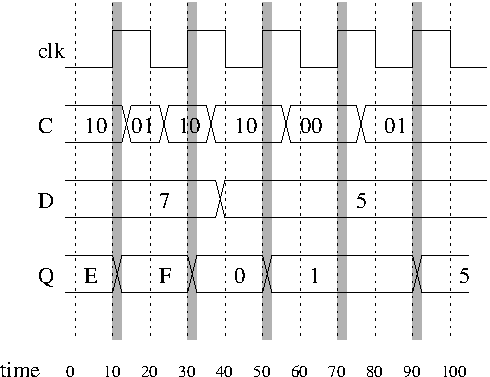
\includegraphics[max width=\textwidth, center]{Sol6-11}
            \else 
\includegraphics[max width=\textwidth, center]{Prob6-11} \fi
            \caption{The timing diagram for a 4-bit arithmetic shift register
            in Problem~\ref{item:shifter}.}
            \label{fig:hwshift}
        \end{figure}

        \needspace{2in}
    \item\textbf{ (5 pts.)} Complete the timing diagram in Figure~\ref{fig:hwcount}
        \label{item:counter}
        for a 4-bit counter.  Use the control setting from the truth table on
        page~\pageref{6-page:counter}.
        \begin{figure}[ht]
            \ifshowanswers 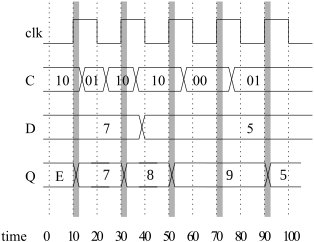
\includegraphics[max width=\textwidth, center]{Sol6-12}
            \else \includegraphics[max width=\textwidth, center]{Prob6-12} \fi
            \caption{The timing diagram for a 4-bit counter in
            Problem~\ref{item:counter}.}
            \label{fig:hwcount}
        \end{figure}

    \item\textbf{ (5 pts.)} Complete the timing waveforms for $A_1, A_0, Q_1, Q_0$
        \label{item:cascade}
        based on the circuit diagram shown in Figure~\ref{fig:cascade}.  Use the truth
        table on page~\pageref{6-page:reg} for the register. Put the decimal
        representation of the signals in the timing diagram (like the timing
        diagram in Figure~\ref{6-fig:sequentialBBcomb1} of the textbook).\needspace{2.2in}
        \begin{figure}[ht]
            \ifshowanswers \includegraphics[max width=\textwidth, center]{Prob6-13}
            \else \includegraphics[max width=\textwidth, center]{Prob6-13} \fi
            \caption{The circuit diagram and incomplete timing diagram for
            Problem~\ref{item:cascade}.}
            \label{fig:cascade}
        \end{figure}

        \needspace{2in}
    \item\textbf{ (4 pts.)} The circuit shown in Figure~\ref{fig:fib} generates a
        Fibonacci sequence, a sequence starting with 1,1,2,3...  The next number in
        the sequence is the sum of the preceding two numbers.  Complete the
        timing diagram, assuming the circuit starts with the values shown.
        Identify the signal which generates a complete Fibonacci sequence.

        \begin{figure}[ht]
            \center{\includegraphics{fib}}
            \caption{A circuit which generates a Fibonacci sequence.}
            \label{fig:fib}
        \end{figure}

\end{enumerate}


%\setcounter{chapter}{7}
%\setcounter{section}{-1}
\chapter{Finite State Machines}
\section{Exercises}
\label{section:finiteStateMachines}
\graphicspath{ {./chapter07/FigHw} }

\begin{enumerate}
    \item A finite state machine has been implemented with four
        flip-flops, two inputs and three outputs.
        \begin{enumerate}
            \item What are the minimum and maximum number of states in the diagram?
                \begin{onlysolution}  \textbf{Solution} \itshape{
                        Since there are three flip flops we can have a maximum of 8 states.  The minimum
                        number of states is a bit tricky.  A practical answer is 5, because if you
                        had fewer states you would use fewer flip flops.  However, the question
                        asks for a minimum, in which case you could have 1 state.  Note, that a
                        1 state FSM would only generate a single output and hence would not be a
                        very interesting circuit.
                    }
                \end{onlysolution}
            \item What are the minimum and maximum number of transition arrows
                starting at a particular state?
                \begin{onlysolution}  \textbf{Solution} \itshape{
                        These values are the same.  Since there are two bits of input there are four
                        different inputs that can be applied at each state.  Thus, four arrows must
                        leave each state.
                    }
                \end{onlysolution}
            \item What are the minimum and maximum number of transition arrows
                ending in a particular state?
                \begin{onlysolution}  \textbf{Solution} \itshape{
                        In a typical design your systems will have a reset state, it normal for such
                        states to have NO input arcs.  You only visit them when the power is turned on.
                        This is the minimum number of arcs that can terminate at a state.  On the
                        other hand, I could image a machine where   transition arc points to a
                        particular state (not a very interesting FSM).  Hence all 32 arcs could point
                        to a single state.
                    }
                \end{onlysolution}
            \item What are the minimum and maximum number of different binary patterns
                that are displayed on the outputs?
                \begin{onlysolution}  \textbf{Solution} \itshape{
                        this is a tricky question, you need to determine which of the inputs and outputs
                        constrains the number of distinct patterns on the output.  You should consult
                        figure 7.1 for some guidance.  There are three bits of output which have the possibility
                        of generating 8 different outputs.  There are a total of six bits of input to the
                        combinational logic box, more than enough to cope with the 8 different output.  On
                        the other end of the scale, I can imagine a FSM which only produces a single output,
                        it would however, not be very interesting.
                    }
                \end{onlysolution}
        \end{enumerate}

    \item \textbf{ (20 points)}
        The state assignment for a FSM influences the amount of
        combinational logic required in the realization.  In the following
        problem this phenomena is investigated.  Determine the MIEs
        for the following state table using
        both the state assignments.

        \begin{tabular}{lll}
            State Table & State Assignment 1 & State Assignment 2  \\
            \begin{tabular}{c|c|c}
                CS x & 0    & 1    \\ \hline
                A    & A,0  & B,0  \\ \hline
                B    & C,1  & F,1  \\ \hline
                C    & D,0  & C,0  \\ \hline
                D    & A,1  & H,1  \\ \hline
                E    & F,1  & E,1  \\ \hline
                F    & G,0  & F,0  \\ \hline
                G    & G,1  & C,1  \\ \hline
                H    & D,1  & E,1  \\
            \end{tabular}
            &
            \begin{tabular}{c||c|c|c}
                State & $Q_2$ & $Q_1$ & $Q_0$ \\ \hline
                A     & 0     & 0     & 0     \\ \hline
                B     & 0     & 0     & 1     \\ \hline
                C     & 0     & 1     & 1     \\ \hline
                D     & 0     & 1     & 0     \\ \hline
                E     & 1     & 0     & 0     \\ \hline
                F     & 1     & 0     & 1     \\ \hline
                G     & 1     & 1     & 1     \\ \hline
                H     & 1     & 1     & 0     \\
            \end{tabular}
            &
            \begin{tabular}{c||c|c|c}
                State & $Q_2$ & $Q_1$ & $Q_0$ \\ \hline
                A     & 0     & 0     & 0     \\ \hline
                B     & 1     & 1     & 1     \\ \hline
                C     & 0     & 0     & 1     \\ \hline
                D     & 1     & 1     & 0     \\ \hline
                E     & 1     & 0     & 1     \\ \hline
                F     & 0     & 1     & 1     \\ \hline
                G     & 1     & 0     & 0     \\ \hline
                H     & 0     & 1     & 0     \\
            \end{tabular}
        \end{tabular}

        After obtaining the MIEs for both realizations, determine the cost
        of each solution according to the following formula:
        $C(FSM) = A + O + 6*F$.  Where $C(FSM)$ denotes
        the cost of the FSM,
        $A$ is the cost of the AND gates,
        $O$ is the cost of the OR gates, and
        $F$ is the number of flip flops.
        The cost of an AND gate is equal to the number of inputs to the
        AND gate.  Likewise the cost of an OR gate is equal to the number
        of inputs.  NOT gates are free. For example, the circuit
        $A'B + ABC'$ costs $(2+3)+2+0=7$.

        Submit:
        \begin{enumerate}
            \item Shared steps of the design process. \ifshowanswers \textit{\color{red}What are you expecting students to give for this?} \fi
            \item Derive the MIEs for each of the two realizations.
                \begin{onlysolution}  \textbf{Solution} \itshape{

                        State Assignment 1

                        \begin{tabular}{l|l|l|l|l}
                            $Q_2 Q_1 \ Q_0 x$  & 00 & 01  & 11 & 10 \\ \hline
                            00  & 000,0 & 001,0 & 101,1 & 011,1  \\ \hline
                            01  & 000,1 & 110,1 & 011,0 & 010,0  \\ \hline
                            11  & 010,1 & 100,1 & 011,0 & 111,1  \\ \hline
                            10  & 101,1 & 100,1 & 101,0 & 111,0  \\
                        \end{tabular}\vspace{-1em}
                        \begin{flalign*}
                            D_2 &= Q_1Q_0'X + Q_1'Q_0X + Q_2Q_0X' + Q_2Q_1'          &&\\
                            D_1 &= Q_2Q_1X' + Q_2'Q_1X + Q_1Q_0 + Q_0X'              &&\\
                            D_0 &= Q_2Q_1'X' + Q_2'Q_1'X + Q_1'Q_0 + Q_2Q_0 + Q_0X   &&\\
                            Z   &= Q_2'Q_1'Q_0 + Q_1Q_0' + Q_2Q_0' + Q_2Q_1          &&
                        \end{flalign*}

                        State Assignment 2

                        \begin{tabular}{l|l|l|l|l}
                            $Q_2 Q_1 \ Q_0 x$  & 00 & 01  & 11 & 10 \\ \hline
                            00  & 000,0 & 111,0 & 001,0 & 110,0  \\ \hline
                            01  & 110,1 & 101,1 & 011,0 & 100,0  \\ \hline
                            11  & 000,1 & 010,1 & 011,1 & 001,1  \\ \hline
                            10  & 100,1 & 001,1 & 101,1 & 011,1  \\
                        \end{tabular}\vspace{-1em}
                        \begin{flalign*}
                            D_2 &= Q_2Q_1'Q_0'X' + Q_2Q_1'Q_0X + Q_2'Q_1Q_0' + Q_2'Q_0'X + Q_2'Q_0X'   &&\\
                            D_1 &= Q_2'Q_1Q_0'X' + Q_2'Q_1'Q_0'X + Q_2Q_1X+Q_1Q_0X + Q_1'Q_0X'         &&\\
                            D_0 &= Q_1'X + Q_2'X + Q_2Q_0                                              &&\\
                            Z   &= Q_1Q_0' + Q_2                                                       &&
                        \end{flalign*}

                    }
                \end{onlysolution}

            \item Determine the cost of each of the two realizations.

                \begin{onlysolution}  \textbf{Solution} \itshape{
                        \begin{tabular}{l|l|l}
                            & State Assignment 1    & State Assignment 2 \\ \hline
                            $D_2$    &     15        &    22    \\ \hline
                            $D_1$    &    14        &    22    \\ \hline
                            $D_0$    &    17        &    9    \\ \hline
                            $Z$    &    13        &    4    \\ \hline
                            Total    & 6*3 + 59 = 77         & 6*3 + 57 = 75    \\
                        \end{tabular}
                    }
                \end{onlysolution}
            \item Determine the cost of each of the two realizations using Espresso.
                \begin{onlysolution}  \textbf{Solution} \itshape{
                        Espresso cost 77 for state assignment  1 \\
                        Espresso cost 75 for state assignment  2
                    }
                \end{onlysolution}
        \end{enumerate}

    \item \textbf{ (8 pts.)} Realize the FSM in the previous problem using
        a one-hot encoding.  Determine
        the MIEs and the cost of the circuit using the same metric.
        It is helpful to convert the state table into a state diagram.
        \begin{onlysolution}  \textbf{Solution} \itshape{
                \begin{description}
                    \item $D_A = Q_AX' + Q_DX'$
                    \item $D_B = Q_AX$
                    \item $D_C = Q_BX'+Q_CX+Q_GX$
                    \item $D_D = Q_CX'+Q_HX'$
                    \item $D_E = Q_EX+Q_HX$
                    \item $D_F = Q_BX+Q_EX'+Q_FX$
                    \item $D_G = Q_FX'+Q_GX'$
                    \item $D_H = Q_DX$
                    \item $Z   = Q_B + Q_D + Q_E + Q_G + Q_H$
                \end{description}

                The cost of this solution is 6*8 + 6 + 2 + 9 + 6 + 6 + 9 + 6 + 2 + 5 = 48 + 51 = 99
            }
        \end{onlysolution}

    \item \textbf{ (8 points)}
        Enhance the vending machine discussed in this chapter as follows.
        Add two buttons for a beverage selection; \textit{ regular} soda and \textit{ diet}
        soda, see Figure~\ref{fig:Vend}.  This machine will have a change dispenser.
        If the user deposits more than 35\textcent, the circuit should send a signal to
        either the \textit{ nickel change} dispenser or the \textit{ dime change} dispenser,
        a single bit sent for one clock cycle to a dispenser will yield a single coin.
        When the user deposits 35\textcent (or more) the machine gives any change and
        then waits for one of the two buttons to be depressed.  Depending on the
        selection, the circuit should send a signal to either the
        \textit{ regular dispenser} or
        the \textit{ diet dispenser} mechanism.  The dispenser need only get a signal for
        one clock cycle.  After the dispensing, go back to the reset state.
        \begin{figure}[ht]
            \center{\includegraphics{Prob7-4}}
            \caption{A basic vending machine.}
            \label{fig:Vend}
        \end{figure}\vspace{-1em}
        \begin{onlysolution}  \textbf{Solution} \itshape{
                \begin{figure}[ht]
                    \includegraphics[max width=\textwidth, center]{Sol7-4}
                \end{figure}

                Note, that in the figure if a input does not appear on
                any arc emanating from a state then it is implied that
                this input will have no effect on the next state.  Below
                are the outputs for each of the states above.

                \begin{tabular}{|l||l|l|l|} \hline
                    \multicolumn{4}{|c|}{outputs from the vending FSM}                      \\ \hline \hline
                    state   & nickel change     & diet dispense     & regular dispense      \\ \hline
                    & 0 give none       & 0 give none       & 0 given none          \\ \hline
                    & 1 give nickel     & 1 dispense diet   & 1 dispense regular    \\ \hline
                    &                   &                   &                       \\ \hline
                    0       & 0                 & 0                 & 0                     \\ \hline
                    5       & 0                 & 0                 & 0                     \\ \hline
                    10      & 0                 & 0                 & 0                     \\ \hline
                    15      & 0                 & 0                 & 0                     \\ \hline
                    20      & 0                 & 0                 & 0                     \\ \hline
                    25      & 0                 & 0                 & 0                     \\ \hline
                    30      & 0                 & 0                 & 0                     \\ \hline
                    35      & 0                 & 0                 & 0                     \\ \hline
                    40      & 1                 & 0                 & 0                     \\ \hline
                    d       & 0                 & 1                 & 0                     \\ \hline
                    r       & 0                 & 0                 & 1                     \\ \hline
                \end{tabular}
            }
        \end{onlysolution}

    \item \textbf{ (6 pts.)}
        Build a FSM for a car alarm.  The input to the FSM
        comes from a tilt sensor.  The tilt-sensor outputs 1 when the
        car has been physically displaced by a preset amount, otherwise the
        tilt sensor outputs 0.  The output of the circuit drives an alarm,
        when the alarm output equals 1 the alarm sounds, otherwise the alarm
        does not sound.  Once the alarm has been set off, it will continue
        sounding until a reset input equals 1, at which point the alarm will
        stop sounding.

        Draw the state diagram and from this determine the MIEs and OEs.

        \begin{onlysolution}
            \includegraphics[center]{Sol7-5}
            \textbf{MIE:}
            \begin{flalign*}
                D_{off} &= Q_{off}Tilt' +  Q_{on}Reset &&\\
                D_{on}  &= Q_{off}Tilt\  + Q_{on}Reset' &&
            \end{flalign*}
            \textbf{OE:}
            \begin{flalign*}
                Alarm\ &= D_{on}  &&\\
                Alarm' &= D_{off} &&
            \end{flalign*}
        \end{onlysolution}
    \item \textbf{ (12 pts.)}
        Build a digital circuit which controls an automatic garage door opener.
        The garage door circuit has three bits of input.  The first input, called
        $button$, comes from a the main control button used to open or close the
        garage door.  When pressed $button=1$ otherwise $button=0$.  The garage
        door rides in a track, at the top and bottom of of which are two
        limit switches.  The top limit switch equals 1 when the garage door
        is all the way up, otherwise its output equals 0.  The bottom limit
        switch equals 1 when the garage door is all the way down, otherwise
        its output equals 0.  The garage door circuit has two bits of output
        called $motor$.  When $motor=01$, the motor moves the door in a downward
        motion, closing the door.  When $motor=10$, the motor moves the door
        upward, opening the garage door.  When $motor=00$, the motor is turned off.

        \begin{figure}[ht]
            \center{\includegraphics{Prob7-6}}
            \caption{The garage door and the circuit controlling it.}
            \label{fig:hwgarage}
        \end{figure}

        Construct the FSM assuming a one-hot encoding of the states.
        Determine the memory input equations and output equations.

        \begin{onlysolution}  \textbf{Solution:} \itshape{
                \begin{itemize}
                    \item\textbf{Control unit}
                        The control unit includes so called wait states.  Waits states are
                        a result of the fact that the clock running the FSM is usually
                        much faster than the physical phenomena being monitored by the FSM.
                        Unless told otherwise, you can assume that any FSM that you are
                        building has a clock which operates on the order of megahertzs.
                        This means that the resulting FSM can make around 1 million
                        state transitions per second.  Clearly, a garage door needs more
                        than one millionth of a second to open or close.  Consequently,
                        the FSM in this problem needs to wait for the door to be opened.
                        This is done by having the FSM repetitively check the status of the
                        door via the up or down limit switches.  In addition to waiting
                        for the garage door to open and close the FSM must wait for a
                        button press.

                        \begin{figure}[ht]
                            \center{\includegraphics{Sol7-6}}
                            \caption{The FSM for the garage door controller.}
                        \end{figure}

                        The state diagram for the garage door controller has four states.
                        In the open and close state, the FSM is waiting for a button push,
                        while the button is not pressed the door stays open or closed.  As
                        soon as the button is pressed the door starts to open or close.
                        It stays in this state until the limit switches tell the FSM that
                        the door has reached the limit of its travel.

                    \item\textbf{Memory Input Equations}
                        Since we are building the garage door controller assuming a
                        one hot encoding of the states, each state will get its own
                        flip flop.  Each flip flop will output a 1 when the FSM is
                        in that state.  The memory input equations for a particular
                        state are determined by answering, ``how do you get into that
                        state?" The four answers to this questions are provided below.

                        {\addtolength{\tabcolsep}{-0.4em}
                            \begin{tabular}{lll}
                                $D_{open}     $&$=\, Q_{open}button'  $&$+\, Q_{opening}up$ \\
                                $D_{close}    $&$=\, Q_{close}button' $&$+\, Q_{closing}down$ \\
                                $D_{opening}  $&$=\, Q_{close}button  $&$+\, Q_{opening}up'$ \\
                                $D_{closing}  $&$=\, Q_{open}button   $&$+\, Q_{closing}down'$ \\
                        \end{tabular}}

                    \item\textbf{Output Equations}
                        The outputs for complex FSMs are usually not written inside the
                        states, rather a separate table is constructed which contains the
                        output for each state.   Even though this is a simple example
                        we will construct an output table.

                        \begin{tabular}{l|l}
                            State    & motor        \\ \hline
                            & 00 stop    \\ \hline
                            & 01 down    \\ \hline
                            & 10 up        \\ \hline
                            open    & 00         \\ \hline
                            close   & 00        \\ \hline
                            opening & 10         \\ \hline
                            closing & 01         \\
                        \end{tabular}

                        Call the outputs $Z_{m1}$ and $Z_{m0}$, for the most and least
                        significant bits of the output respectively.  Then the outputs
                        are determined by asking for which states does the output
                        equal 1?  The answers to this question are shown below.

                        \begin{tabular}{l}
                            $Z_{m1} = Q_{opening}$ \\
                            $Z_{m0} = Q_{closing}$ \\
                        \end{tabular}
                \end{itemize}
            }
        \end{onlysolution}

    \item \textbf{ (8 pts.)}
        Build a digital circuit to control a single traffic light.  The circuit
        has three outputs, $Rlight, Ylight$ and $ Glight$.  When
        $Rlight=1$ the red light illuminates otherwise the light is off.
        The same behavior holds true for $Ylight$ and $Glight$.  In order
        to sequence the lights, the circuit has three timers, Rtimer, Gtimer and
        Ytimer.  Each timer controls the length of time that its light should be
        illuminated.  Each timer has one bit of input and one bit of output.  When a
        timer's input is 0, the timer is reset.  When a timer's one bit
        input is 1, the timer
        counts down its preset timer interval.  When a timer counts all the way down,
        its output goes to 1 and stays there until the timer is reset (by applying
        an input of 0).  The state diagram of the circuit is shown in the
        figure below.  As shown in figure~\ref{fig:TrafficFSM} the FSM receives input from the
        three timers, while the output of the FSM controls the counters. Complete
        the following three tasks.
        \begin{figure}[t]
            \ifshowanswers \includegraphics[max width=\textwidth, center]{Sol7-7}
            \else \includegraphics[max width=\textwidth, center]{Prob7-7} \fi
            \caption{}
            \label{fig:TrafficFSM}
        \end{figure}

        \begin{enumerate}
            \item Label the arcs of the FSM with the input values (Rt, Yt or Gt)
                needed to make the circuit operate correctly.

            \item Next, determine what the output should be in each
                of the states.  Instead of writing the output in each state, the
                outputs are organized in a separate table.  In this table, each
                row will contain the output associated with a particular state.
                Each column in the table will be associated with one bit of the output.

                \begin{onlyproblem}
                    \begin{tabular}{l||l|l|l|l|l|l}state&Rlight&Ylight&Glight&Rtimer&Ytimer&Gtimer\\\hline&0~off&0~off&0~off&0~rst&0~rst&0~rst\\\hline&1~on&1~on&1~on&1~run&1~run&1~run\\\hline\hline R&&&&&&\\\hline Y&&&&&&\\\hline G&&&&&&\\
                    \end{tabular}
                \end{onlyproblem}
                \begin{onlysolution}
                    \begin{tabular}{l||l|l|l|l|l|l}
                        state         & Rlight & Ylight & Glight & Rtimer & Ytimer & Gtimer    \\ \hline
                        & 0 off  & 0 off  & 0 off  & 0 rst  & 0 rst  & 0 rst    \\ \hline
                        & 1 on   & 1 on   & 1 on   & 1 run  & 1 run  & 1 run    \\ \hline \hline
                        R             & 1      & 0      & 0      & 1      & 0      & 0        \\ \hline
                        Y             & 0      & 1      & 0      & 0      & 1      & 0        \\ \hline
                        G             & 0      & 0      & 1      & 0      & 0      & 1        \\
                    \end{tabular}
                \end{onlysolution}

            \item Finally, write the memory input equations and output
                equations for the traffic light controller.  In order to write the
                memory input equations use the labels on the state transitions from
                the state diagram.   In order to write the output equations
                use the output table.

                \begin{onlyproblem}
                    \begin{tabular}{p{2in}p{2in}}
                        \begin{tabular}{l@{}l}$Q_{red}$&$=$\\$Q_{yellow}\,$&$=$\\$Q_{green}$&$=$\\
                        \end{tabular}&
                        \begin{tabular}{l@{}l}$Z_{Rlight}$&$=$\\$Z_{Ylight}$&$=$\\$Z_{Glight}$&$=$\\$Z_{Rtimer}$&$=$\\$Z_{Ytimer}$&$=$\\$Z_{Gtimer}\,$&$=$\\
                        \end{tabular}
                    \end{tabular}
                \end{onlyproblem}
                \begin{onlysolution}{\color{blue}
                        \begin{tabular}{p{2in}p{2in}}
                            \begin{tabular}{l@{}l} % @{} removes all automatic padding from the table
                                $D_{red}$      & $=Q_{Set30} + Q_{Red   }Rt$    \\
                                $D_{yellow}\,$ & $=Q_{Set5 } + Q_{Yellow}Yt$    \\ % Manually creating alignment removes the spacing around symbols, so artificially add it back on longest line
                                $D_{green}$    & $=Q_{Set25} + Q_{Green }Gt$    \\
                            \end{tabular}
                            &
                            \begin{tabular}{l@{}l}
                                $Z_{Rlight}$   & $= Q_{Red   }$ \\
                                $Z_{Ylight}$   & $= Q_{Yellow}$ \\
                                $Z_{Glight}$   & $= Q_{Green }$ \\
                                $Z_{Rtimer}$   & $= Q_{Red   }$ \\
                                $Z_{Ytimer}$   & $= Q_{Yellow}$ \\
                                $Z_{Gtimer}\,$ & $= Q_{Green }$ \\
                            \end{tabular}
                    \end{tabular}}
                \end{onlysolution}
        \end{enumerate}
        \filbreak
    \item \textbf{ (16 pts.)}
        Build a FSM which make the hexapod robot shown in Figure~\ref{fig:hexapod}
        walk forward.

        \begin{figure}[ht]
            \center{\includegraphics{Prob7-8}}
            \caption{A hexapod walking robot.}
            \label{fig:hexapod}
        \end{figure}

        Each leg of the hexapod robot is moved by two nitinol (Flexinol) wires.
        At rest, nitinol wire is straight.  When 5 volts (logic 1) is applied to
        the wire, it bends in a particular direction.  The two wires making up
        a particular leg are positioned so that they move in perpendicular
        directions.  One wire moves a leg up or down and the other will move
        the wire forward or backwards.  The table below elaborates.

        \begin{tabular}{l|l|l}
            wire   & logic 0 & logic 1    \\ \hline
            $w_0$  & down     & up        \\ \hline
            $w_1$  & forward & backward    \\
        \end{tabular}

        The hexapod robot walks by moving three legs in unison; see $A$ and
        $B$ in Figure~\ref{fig:hexapod}.  The movements of $A$ and $B$ are
        coordinated so that, at times, the hexapod is balanced on three legs.
        A portion of the walking gait is shown in Figure~\ref{fig:hexgate};
        note that in this figure the viewer is looking down at the top of the
        robot which is moving to the right.  The dotted legs are assumed to be in
        the air, solid legs are in contact with the ground.

        \begin{figure}[ht]
            \center{\includegraphics{Prob7-8b}}
            \caption{The walking gait of the hexapod robot.}
            \label{fig:hexgate}
        \end{figure}

        Assume that the legs can move to their correct position in one clock
        cycle.  Define each state as a position of the legs in
        Figure~\ref{fig:hexgate}. Draw the state diagram,
        and determine the memory input and output equations.

        \begin{onlysolution}\filbreak  \textbf{Solution} \itshape{

                \includegraphics[max width=\textwidth, center]{Sol7-8}
                Note that the states have been given numbers to simplify the
                description of the states.  Here is a listing of the outputs
                associated with each state:

                \begin{tabular}{l|l|l|l|l}
                    State  & $Aw_1$ & $Aw_0$ & $Bw_1$ & $Bw_0$  \\ \hline
                    1    & 0    & 0     & 1      & 1        \\ \hline
                    2    & 1    & 0     & 0      & 1        \\ \hline
                    3    & 1    & 1     & 0      & 0        \\ \hline
                    4    & 0    & 1     & 1      & 0        \\
                \end{tabular}

                \textbf{ MIEs and OEs}

                \begin{tabular}{ll}
                    MIEs        &    OEs            \\
                    $D_1 = Q_4$    &    $Z_{Aw_1} = Q_2 + Q_3$    \\
                    $D_2 = Q_1$    &    $Z_{Aw_0} = Q_3 + Q_4$    \\
                    $D_3 = Q_2$    &    $Z_{Bw_1} = Q_1 + Q_4$    \\
                    $D_4 = Q_3$    &    $Z_{Bw_0} = Q_1 + Q_2$    \\
                \end{tabular}

            }
        \end{onlysolution}

    \item \textbf{ (12 pts.)}
        \label{item:robot}
        Build a FSM which makes the simple robot shown in Figure~\ref{fig:Robot}
        move along (track) the black line crossing two intersections.
        \begin{figure}[ht]
            \includegraphics[max width=\textwidth, center]{Prob7-9}
            \caption{A simple line-tracking robot that must cross two intersections.}
            \label{fig:Robot}
        \end{figure}

        The FSM has two inputs, a left sensor, denoted \textit{ ls}, and a right
        sensor, denoted \textit{ rs}.  These two sensors look down at the ground.
        When a sensor sees white, it outputs 0; when it see black, it outputs 1.
        The sensors are spaced far enough apart that they can straddle the black
        line and see white on either side.  The FSM has two outputs, a left
        motor, denoted \textit{ lm} and a right motor, denoted \textit{ rm}.  A motor
        rotates when it is sent a 1 and does not rotate when it is sent a 0.
        The FSM should constantly check that the robot is straddling the line.
        If it is not the FSM should take corrective action by stopping one of
        the wheels.

        Submit the state diagram for the FSM,  MIEs and OEs using
        a one-hot encoding of the states.

        \begin{onlysolution}  \textbf{Solution} \itshape{

                \textbf{FSM}

                \includegraphics[max width=\textwidth, center]{Sol7-9}
                \begin{tabular}{l|l|l|l}
                    State    & lm                & rm                  \\ \hline
                    & 0 stop left wheel & 0 stop right wheel  \\ \hline
                    & 1 turn left wheel & 1 turn right wheel  \\ \hline
                    &                   &                     \\ \hline \hline
                    Reset    & 1                 & 1                   \\ \hline
                    Straight & 1                 & 1                   \\ \hline
                    Left     & 0                 & 1                   \\ \hline
                    Right    & 1                 & 0                   \\ \hline
                    OnLine   & 1                 & 1                   \\ \hline
                    Done     & 0                 & 0                   \\
                \end{tabular}
            }
            {\color{blue}
                \textbf{MIE}
                \begin{align*}
                    D_{S }    &= Q_{Reset} + Q_{S}(ls'*rs') + Q_{L}(ls'*rs') + Q_{R}(ls'*rs') + Q_{OL}(ls+rs)\\
                    D_{L }    &= Q_{S}(ls*rs') \\
                    D_{R }    &= Q_{S}(ls'*rs) \\
                    D_{OL}    &= Q_{L}(ls*rs)  + Q_{R}(ls*rs) + Q_{S}(ls*rs) + Q_{OL}(ls*rs)\\
                    D_{Done} &=  Q_{OL}(ls+rs) + Q_{Done}
                \end{align*}
                \textbf{OE}
                \begin{align*}
                    Z_{lm} &= Q_{Reset} + Q_{S} + Q_{R} + Q_{OL}\\
                    Z_{rm} &= Q_{Reset} + Q_{S} + Q_{L} + Q_{OL}
            \end{align*}}
        \end{onlysolution}

    \item \textbf{ (16 pts.)}
        Make the robot from Problem \ref{item:robot} cross 63 intersections.
        The problem is that the number of states will grow to large to handle
        with a FSM by itself.  Additional hardware, in the form of a counter
        and comparator, are added to the FSM to address this problem.

        \begin{figure}[ht]
            \center{\includegraphics[max width=\textwidth, center]{Prob7-10}}
            \caption{The innards of a intersection counting, line tracking robot.}
            \label{fig:linecounter}
        \end{figure}

        Assume that the counter is reset to 0 when the circuit
        is first turned on.  The robot must still track the line, but
        must also count up once every time it crosses an intersection.  Remember
        the digital circuit shown in Figure~\ref{fig:linecounter} is
        operating much faster than the robot is crossing intersections.
        \filbreak
        The state diagram needs to have wait states while it crosses
        the intersection, similar to those
        in the DAISY example.  Assume the counter counts up
        when the control input is 1 and the clock rises.  When the control
        input is 0, then the counter holds its current count value.

        Submit the state diagram for the FSM, OEs and MIEs for a one-hot
        encoding of the states.

        \begin{onlysolution}  \textbf{Solution} \itshape{
                If you encoded 64 line crossing using only a FSM you would have
                on the order of 256 states, 4 for each line crossing.  The solution
                is to use a counter to keep track of how many lines have been crossed.
                The states below explain.

                \textbf{FSM}

                \includegraphics[max width=\textwidth, center]{Sol7-10}

                \filbreak
                \textbf{ Control Word}

                \begin{tabular}{l|l|l|l}
                    State    & lm                & rm                  & counter \\ \hline
                    & 0 stop left wheel & 0 stop right wheel  & 00 hold \\ \hline
                    & 1 turn left wheel & 1 turn right wheel  & 01 load \\ \hline
                    &                   &                     & 10 count\\ \hline \hline
                    Reset    & 1                 & 1                   & 01      \\ \hline
                    Straight & 1                 & 1                   & 00      \\ \hline
                    Left     & 0                 & 1                   & 00      \\ \hline
                    Right    & 1                 & 0                   & 00      \\ \hline
                    OnLine   & 1                 & 1                   & 00      \\ \hline
                    Up       & 1                 & 1                   & 10      \\ \hline
                    Stop     & 0                 & 0                   & 00      \\
                \end{tabular}

                { \color{blue}
                    \textbf{MIE}
                    \begin{flalign*} % flalign both sets as these are almost the width of the page
                        D_{S }   &= Q_{Reset} + Q_{S}(ls'*rs') + Q_{L}(ls'*rs') + Q_{R}(ls'*rs') + Q_{Up}(L)\\
                        D_{L }   &= Q_{S} (ls*rs') \\
                        D_{R }   &= Q_{S} (ls'*rs) \\
                        D_{OL}   &= Q_{L} (ls*rs)  + Q_{R}(ls*rs) + Q_{S}(ls*rs) + Q_{OL}(ls*rs)\\
                        D_{Up}   &= Q_{OL}(ls+rs)  &\\
                        D_{Stop} &= Q_{Up}(L') &
                    \end{flalign*}
                    \textbf{OE}
                    \begin{flalign*}
                        Z_{lm } &= Q_{Reset} + Q_{S} + Q_{R}  + Q_{OL} &\\
                        Z_{rm } &= Q_{Reset} + Q_{S} + Q_{L}  + Q_{OL} &\\
                        Z_{c_1} &= Q_{Up} & \\
                        Z_{c_0} &= Q_{Reset} &
                \end{flalign*}}
            }
        \end{onlysolution}

    \item \textbf{ (24 pts.)}
        Construct a digital circuit to control the operation of a
        simple washing machine, see Figure~\ref{fig:Wash}.
        \begin{figure}[ht]
            \includegraphics[max width=\textwidth, center]{Prob7-11}
            \caption{A humble washing machine with a close-up of the start
            button and temperature switch.}
            \label{fig:Wash}
        \end{figure}

        To use the simple washing machine set the temperature switch to
        either hot, tepid or cold and then press the start button.
        To build a digital circuit to control the washing of clothes
        its necessary to understand the washing cycle.  When the start
        button is pressed water of the selected temperature pours
        into the washing drum.  The simple washing machine has two
        electronically controlled water valves, the hot valve admits
        hot water into the washing drum and the cold valve admits
        cold water.  Water continues to pour into the drum until it
        fills.  There are two water level sensors; the full switch signals when
        the drum is full of water and the empty switch signals when the drum
        is empty.  After the drum is full of water the simple washing machine
        starts to agitate the clothes.  The simple washing machine has a motor
        controlled by two bits, which agitates (a rapid back and forth motion),
        spins (a rapid rotation in one direction) or does nothing.  After
        agitating for 15 minutes, the agitation cycle stops and
        the machine drains its water.  Water leaves the drum through
        a drain valve.  When the drum is emptied of water the washing machine enters
        the rinse cycle.   The rinse cycle fills the drum with cold
        water and agitates for 5 minutes.  The rinse cycle concludes
        by draining the water from the drum.
        When the drum is emptied of water the washing machine enters
        the spin cycle.  This lasts for 5 minutes.  The simple washing machine
        keeps track of time  using a 5 minute timer.   To use the timer
        it must first be reset for one clock cycle.  After being reset the
        timer will count down as long as the timer input is set to run.
        After 5 minutes have elapsed the timer output will go to logic 1 and
        stay there until the timer is reset.  In order to get longer time
        intervals, the timer should be reset for another 5 minutes and count
        down again.  When the spin cycle is done, the washing is complete. The
        inputs from the washing machine to the digital circuit have the
        following meaning.

        \begin{tabular}{|l|l|l|l|l|} \hline
            \multicolumn{5}{|c|}{inputs to the digital circuit}        \\ \hline \hline
            start & temperature & empty       & full       & timer out     \\ \hline
            0 off & 00 hot      & 0 not empty & 0 not full & 0 nothing    \\ \hline
            1 on  & 01 cold     & 1 empty     & 1 full     & 1 5 minutes elapsed     \\ \hline
            & 10 tepid    &          &           &        \\ \hline
        \end{tabular}

        The outputs from the digital to the washing machine have the following meaning.
        The left most column is explained below.

        \begin{tabular}{|l|||l|l|l|l|l|} \hline
            \multicolumn{6}{|c|}{outputs from the digital circuit}            \\ \hline \hline
            state & hot     & cold    & motor      & timer in   & drain     \\ \hline
            & 0 close & 0 close & 00 off     & 00 hold    & 0 close    \\ \hline
            & 1 open  & 1 open  & 01 agitate & 01 reset   & 1 open    \\ \hline
            &        &         & 10 spin    & 10 run     &        \\ \hline \hline
            \textbf{ S1}    &    &      &           &        &        \\ \hline
        \end{tabular}

        Draw the state diagram for the FSM to control the washing machine.
        Label the arcs of the state diagram with the input (or its negation)
        that causes the transition.  Use simple Boolean expressions on these
        arcs, for example (start and hot).
        For each state define the output using a table similar to the one above.
        For example, if \textbf{ S1} is a state fill in the bit values for the o
        outputs depending on what state \textbf{ S1} is supposed to do.
        Determine the memory input equations and output equations assuming a one-hot
        encoding.

        \begin{onlysolution}  \textbf{Solution} \itshape{
                % \begin{enumerate} % I'm not sure what most of these mean, or why these are the only deductions listed for any problem
                %     \item No control table (-6)
                %     \item Disposable washing machine (-1)
                %     \item No OEs (-5)
                %     \item start * cold (-2)
                %     \item no complements on arcs (-2)
                % \end{enumerate}
                \begin{figure}[ht]
                    \center{\includegraphics{Sol7-11}}
                    \caption{The FSM for a washing machine.}
                \end{figure}

                \begin{tabular}{|l|||l|l|l|l|l|} \hline
                    \multicolumn{6}{|c|}{outputs from the digital circuit}        \\ \hline \hline
                    state & hot     & cold    & motor      & timer in   & drain   \\ \hline
                    & 0 close & 0 close & 00 off     & 00 nothing & 0 close \\ \hline
                    & 1 open  & 1 open  & 01 agitate & 01 reset   & 1 open  \\ \hline
                    &         &         & 10 spin    & 10 start   &         \\ \hline
                    &         &         &            & 11 stop    &         \\ \hline \hline
                    HOME  &    0    & 0       & 00         & 00         & 0       \\ \hline
                    COLD  &    0    & 1       & 00         & 01         & 0       \\ \hline
                    TEPI  &    1    & 1       & 00         & 01         & 0       \\ \hline
                    HOT   &    1    & 0       & 00         & 01         & 0       \\ \hline
                    AGIT  &    0    & 0       & 01         & 10         & 0       \\ \hline
                    ZERO  &    0    & 0       & 00         & 01         & 0       \\ \hline
                    DRAI  &    0    & 0       & 00         & 01         & 1       \\ \hline
                    SPIN  &    0    & 0       & 10         & 10         & 0       \\ \hline
                \end{tabular}
                \begin{align*}
                    D_{home}   &= Q_{home}start' + Q_{spin}time \\
                    D_{cold1}  &= Q_{home}*start*cold \\
                    D_{tepi}   &= Q_{home}*start*tepid \\
                    D_{hot}    &= Q_{home}*start*hot \\
                    D_{agit1}  &= Q_{cold1}*fill + Q_{tepid}*fill + Q_{hit}*fill + Q_{agit1}*time' \\
                    D_{zero1}  &= Q_{agit1}*time \\
                    D_{agit2}  &= Q_{zero1}*time + Q_{agit2}*time' \\
                    D_{zero2}  &= Q_{agit2}*time \\
                    D_{agit3}  &= Q_{zero2}*time + Q_{agit2}*time' \\
                    D_{drain1} &= Q_{agit3}*time + Q_{drain1}*empty' \\
                    D_{cold2}  &= Q_{drain1}*empty + Q_{cold2}*fill' \\
                    D_{agit4}  &= Q_{cold2}*fill + Q_{agit4}*time' \\
                    D_{drain2} &= Q_{agit4}*time + Q_{drain2}*empty' \\
                    D_{spin}   &= Q_{drain2}*empty + Q_{spin}*time'
                \end{align*}

                {\color{blue}
                    \begin{align*}
                        Z_{hot    } &= Q_{tepid} + Q_{hot}\\
                        Z_{cold   } &= Q_{cold} + Q_{tepid}\\
                        Z_{motor_1} &= Q_{spin}\\
                        Z_{motor_0} &= Q_{agit}\\
                        Z_{timer_1} &= Q_{agit} + Q_{spin}\\
                        Z_{timer_0} &= Q_{cold} + Q_{tepid} + Q_{hot} + Q_{zero} + Q_{drain}\\
                        Z_{drain  } &= Q_{drain}
                \end{align*}}
            }
        \end{onlysolution}

    \item \textbf{ (36 pts.)}
        Construct a digital circuit to control the movement of an elevator in a
        four-story building.  The elevator will always wait on its current floor
        until a call button is pressed; see Figure~\ref{fig:elevator}.  The
        elevator then moves to the floor that was called.  The elevator then
        opens its doors and waits for an elevator control button to be pressed.
        If a a call to another floor is received before an elevator control
        button is pressed, then the elevator closes the doors and goes to the
        new floor.  When a floor is selected on the elevator control panel, then
        the door close and the elevator moves to the desired floor.

        \begin{figure}[ht]
            \center{\includegraphics{Prob7-12}}
            \caption{The layout of an elevator in a four story tall building.}
            \label{fig:elevator}
        \end{figure}

        The inputs to the digital circuit clearly include all the buttons.
        When a button is pressed on the elevators control panel two things
        happen.  A 2-bit binary value representing the button pressed
        becomes valid and a 1-bit panel request becomes valid.  The
        panel request line will remain valid until acknowledged.

        When a call button is pressed two things happen.  A 2-bit binary value
        representing which call button was pressed becomes valid and a 1-bit
        call request becomes valid.  The call request line will remain valid
        until acknowledged.

        Another input tells the circuit when the
        elevator is or is not aligned with a floor.  For example, consider
        an elevator moving from the first to the third floor.  Initially, the
        align variable is 1.  When the elevator starts
        to move away from the first floor towards the second, the align
        variable goes to 0.  When the elevator reaches the second floor, the
        align variable will go to logic 1 and remain there for a short
        while (at least several milliseconds) because there is some
        slack allowed in what is considered ``aligned".  After the elevator
        passes the second floor, the align variable goes back to 0 and stays
        there until the elevator reaches the third floor.

        Here is the table of inputs to the FSM, their abbreviations, to be
        used in the FSM, and their meaning.

        \begin{tabular}{|l|l||l|l|} \hline
            Control panel floor     & Pfloor        & 2-bit floor number & \\ \hline
            Panel request           & Preq          & The panel has a valid floor & \\ \hline
            Call floor              & Cfloor        & 2-bit floor number & \\ \hline
            Call request            & Creq          & The call buttons have a valid floor & \\ \hline
            Align                   & Align         & 0 not aligned & 1 Aligned \\ \hline
        \end{tabular}

        The outputs from the digital circuit to control the door and the
        movement of the elevator.

        \begin{tabular}{|l|l|l|l|} \hline
            Panel acknowledge       & Pack  & Acknowledge the panel request & \\ \hline
            Call acknowledge        & Cack  & Acknowledge the call request & \\ \hline
            Door                    &  0 close &    1 open  &         \\ \hline
            Motor                   &  00 stop &    01 up   & 10 down \\ \hline
        \end{tabular}

        Submit; an algorithm for the datapath and control unit,
        the control word table, the memory input equations, and output equations.
        \begin{onlysolution}[fragile] \color{blue}%required to use verbatim environments inside of an answer
\begin{lstlisting}
uint2_t loc = 0; #Assume starting location
int3_t delta;
while(1) {
    if(Creq){
        Cack = 1;
        Door = 0;

        delta = Cfloor - loc;
        if (delta > 0): Motor[0] = 1;
        if (delta < 0){
            Motor[1] = 1;
            delta = 0 - delta;
        }
        while delta > 0{
            while (Align == 0);
            while (Align == 1);
            delta--;
        }
        Motor[1] = 0;
        Motor[0] = 0;
        Door = 1;
        Cack = 0;
    }
    if(Preq){
        Pack = 1;
        Door = 0;

        delta = Preq - loc;
        if (delta > 0): Motor[0] = 1;
        if (delta < 0){
            Motor[1] = 1;
            delta = 0 - delta;
        }
        while delta > 0{
            while (Align == 0);
            while (Align == 1);
            delta--;
        }
        Motor[1] = 0;
        Motor[0] = 0;
        Door = 1;
    }
}
\end{lstlisting} % This is written with the assumption that it will be turned into logical blocks
            \includegraphics[max width=\textwidth, center]{sol7-12}
        \end{onlysolution}
    \item \textbf{ (36 pts.)}
        Construct a digital circuit to control the movement of traffic
        at the four way intersection shown in Figure~\ref{fig:crossroad}.

        \begin{figure}[ht]
            \center{\includegraphics{Prob7-13}}
            \caption{The layout of a four way intersection.}
            \label{fig:crossroad}
        \end{figure}

        The circuit comes equipped with timers.
        The timer has 2 inputs which set the timer to some preset
        amount of time or allows the timer to count down.  When the
        timer reaches 0 then the output of the timer goes to 1.
        When the timer is not at 0 then the output equals 1.
        The specific inputs and behavior are described in the following
        truth table.

        \begin{tabular}{|c|c|} \hline
            timer input & behavior          \\ \hline \hline
            00 & count down                 \\ \hline
            01 & set to timer to 5  seconds \\ \hline
            10 & set to timer to 15 seconds \\ \hline
            11 & set to timer to 30 seconds \\ \hline
        \end{tabular}

        In addition to the timer there are a variety of real world inputs
        sent to the circuit described in the following table.

        \begin{tabular}{|l|l|l|} \hline
            Name                    & Abbreviation & Function \\                       \hline \hline
            E or W Pressure Sensor  & EW-PS & 1 if 250 lb. or more on E or W sensor \\ \hline
            Ped button              & ped   & 1 if any pedestrian crosswalk button  \\ \hline
        \end{tabular}

        The outputs from the digital circuit to control the lights are:

        \begin{tabular}{|l|l|l|l|} \hline
            light           & 0x red &  10 yellow & 11 green \\ \hline
        \end{tabular}

        The main sequence of events is outlined below;
\begin{verbatim}
while(1) {
    Nlight = Slight = green;
    Elight = Wlight = red;
    wait 30 seconds;
    while ((EW-PS == 0) && (ped == 0));
    Nlight = Slight = yellow;
    wait 5 seconds;
    if (ped == 1) {
        Nlight = Slight = red;
        Elight = Wlight = red;
        wait 15 seconds;
    }
    Nlight = Slight = red;
    Elight = Wlight = green;
    wait 15 seconds;
    Elight = Wlight = yellow;
    wait 5 seconds;
    if (ped == 1) {
        Nlight = Slight = red;
        Elight = Wlight = red;
        wait 15 seconds;
}   }
\end{verbatim}

        Submit;
        the control unit,
        the control word table,
        the memory input equations, and
        output equations.
        \newpage
        \begin{onlysolution}  \textbf{Solution} \itshape{

                \begin{figure}[ht]
                    \center{\includegraphics{Sol7-13}}
                    \caption{The FSM for a traffic light controller.}
                \end{figure}

                \begin{tabular}{|l|||l|l|l|} \hline
                    \multicolumn{4}{|c|}{outputs from the digital circuit}    \\ \hline \hline
                    state & Timer     & NS light  & EWlight     \\ \hline
                    & 00 down   & 00 red    & 00 red      \\ \hline
                    & 01 5 sec  & 01 red    & 01 red      \\ \hline
                    & 10 15 sec & 10 yellow & 10 yellow   \\ \hline
                    & 11 30 sec & 11 green  & 11 green    \\ \hline \hline
                    North    & 00       & 11          & 00  \\ \hline
                    set30 & 11       & 11          & 00  \\ \hline
                    wait30& 00       & 11          & 00  \\ \hline
                    Nwait    & 00       & 11          & 00  \\ \hline

                    YRset5  & 01       & 10          & 00  \\ \hline
                    YRwait5 & 00       & 10          & 00  \\ \hline

                    RRset15 & 10       & 00          & 00  \\ \hline
                    RRwait15& 00       & 00          & 00  \\ \hline

                    RGset15 & 10       & 00          & 11  \\ \hline
                    RGwait15& 00       & 00          & 11  \\ \hline
                \end{tabular}

                The memory input equations are a snap.
                \begin{description}
                    \item $D_{North} = Q_{RYwait5}*ped*timer + Q_{RRwait15}*timer $
                    \item $D_{Set30} = Q_{North} $
                    \item $D_{Wait30} = Q_{Set30} + Q_{Wait30}*timer' $
                    \item $D_{Nwait} = Q_{Wait30}*timer + Nwait*EW_PS'*ped' $
                    \item $D_{YRset5} = Q_{Nwait}*(EW_PS + ped) $
                    \item $D_{YRwait5} = Q_{YRset5} +Q_{YRwait5}*timer' $
                    \item $D_{RRset15} = Q_{YRwait5}*ped*timer $
                    \item $D_{RRwait15} = Q_{RRset15} + Q_{RRwait15}*timer' $
                    \item $D_{RGset15} = Q_{YRwait5}*ped'*timer + Q_{RRwait15}*timer $
                    \item $D_{RGwait15} = Q_{RGset15} $
                    \item $D_{RYset5} = Q_{RGwait15}*timer' $
                    \item $D_{RYwait5} = Q_{RYset5} + Q_{RYwait5}*timer' $
                    \item $D_{RRset15} = Q_{RYwait5}*ped $
                    \item $D_{RRwait15} = Q_{RRset15} +Q_{RRwait15}*timer' $
                \end{description}

                The output equations
                \begin{description}
                    \item $Z_{t1}  = Q_{set30} + Q_{RRset15} $
                    \item $Z_{t0}  = Q_{set30} + Q_{YRset5} $
                    \item $Z_{ns1} = Q_{North} + Q_{set30} + Q_{wait30} + Q_{Nwait} +Q_{YRset5}+Q_{YRwait5} $
                    \item $Z_{ns0} = Q_{North} + Q_{set30} + Q_{wait30} + Q_{Nwait} $
                    \item $Z_{ew1} = Q_{RGset15} + Q_{RGwait15} $
                    \item $Z_{ew0} = Q_{RGset15} + Q_{RGwait15} $
                \end{description}
            }
        \end{onlysolution}
\end{enumerate}


%\setcounter{chapter}{8}
%\setcounter{section}{-1}
\chapter{Datapath and Control}
\section{Exercises}
\label{section:datapathControl}
\graphicspath{ {./chapter08/FigHw} }

\begin{enumerate}
    \item \textbf{ (4 pts.)}
        Show how to eliminate the 4-bit 2:1 mux in the bit counter by assuming
        that the Y register had an asynchronous active low reset input. Consider
        the fact that the external world still needs the ability to hit a single
        button to reset the state of the entire circuit.

    \item  \textbf{ (6 pts.)}
        A control unit has been built with the following control word:

        \begin{tabular}{|c|c|c|c|c|}  \hline
            Reg A   & Reg B   & Reg P  & Mux M      \\ \hline
            00 hold & 00 hold & 1 hold & 1 Load 0   \\ \hline
            11 lsr  & 11 lsr  &        &            \\ \hline
            10 lsl  & 10 lsl  & 0 load & 0 Load Add \\ \hline
            01 load & 01 load &        &            \\ \hline
        \end{tabular}

        Regrettably, these setting were completely wrong.  In reality here is what the control word should
        have been:

        \begin{tabular}{|c|c|c|c|c|}  \hline
            Reg A   & Reg B   & Reg P  & Mux M      \\ \hline
            00 hold & 00 hold & 0 hold & 0 Load 0   \\ \hline
            01 lsr  & 01 lsr  &        &            \\ \hline
            10 lsl  & 10 lsl  & 1 load & 1 Load Add \\ \hline
            11 load & 11 load &        &            \\ \hline
        \end{tabular}

        The design team is in a total panic.
        The design team thinks that it will take weeks to straighten out the error,
        they claim that the control unit needs to be redesigned.  However, there is
        a cheap and easy solution.  Design some combinational
        logic to insert between the faulty control unit and the datapath in order
        to straighten out the bum control signals.  There is one error can be
        fixed by changing something in the datapath, no extra hardware is
        required.  Identify this error and its solution.

        \begin{onlysolution} \textbf{Solution: }
            The mux's control input was flipped. If we change which signal is on what input, the issue will be dealt with.

            To fix the others, we could use the following logic (A and B are the same)
            \begin{align*}
                A_1^* & = A_1 \otimes A_0 \\
                A_0^* & = A_0             \\
                P^*   & = P'
            \end{align*}
        \end{onlysolution}
    \item \textbf{ (8 pts.)}
        Modify the algorithm for the bit counting circuit so that it uses a
        two-line handshake to transmit the Y register.  The circuit should take
        the role of an active producer in the transmission of Y.  The circuit
        has four handshaking lines and two data lines.  Hint, a common
        error of students is to insert a three-state buffer on the output of
        the Y register to the outside world to prevent its transmission to
        the outside world until the value of Y is finalized.  Don't do this!
        If the outside world reads the value of Y before the circuit's signals
        are valid (via the send\_REQ signal) then its their own dumb fault.
        Just send the Y signal outside the datapath as is.

    \item \textbf{ (16 pts.)}
        A 8kx32 RAM is full of integer data.  Design a circuit to scan
        the RAM and find its smallest value.

        Turn in; an algorithm the datapath and control unit, the control word
        table, the memory input equations, and output equations.
        The control unit is to be implemented using a ones hot encoding.

        \begin{onlysolution}[fragile] \textbf{Solution: }
            For this, we need to further expand on section~\ref{8-sec:Minimum Search}

              \begin{verbatim}
1.  min = 0xFFFFFFFF;         // Set the min reg to largest 32-bit value
2.  for (i=0; i<8192; i++) {  // Search through the entire array
3.      MBR=RAM[i];           // Read a value from RAM
4.      if (MBR<min) then     // If MBR is smaller than min
5.          min = MBR;        //   then set min to the smallest value
6.  } // end for
\end{verbatim}
            \textbf{DP \& CU}\\
            \includegraphics[max width=\textwidth, center]{Sol8-4}
            \begin{tabular}{c|c|c|c|c|c}
                \textbf{State}   & enb    & Min Reg & Min mux    & Counter  & MBR Reg \\ \hline
                & 0      & 0 hold  & 0 load FF  & 00 hold  & 0 hold  \\ \hline
                & 1 read & 1 load  & 1 load RAM & 01 load  & 1 load  \\ \hline
                &        &         &            & 10 count &         \\ \hline
                &        &         &            & 11 reset &         \\ \hline
                &        &         &            &          &         \\ \hline
                \textbf{InitMin} & 0      & 1       & 0          & 00       & 0       \\ \hline
                \textbf{InitI}   & 0      & 0       & x          & 01       & 0       \\ \hline
                \textbf{CompC}   & 0      & 0       & x          & 00       & 0       \\ \hline
                \textbf{Read}    & 1      & 0       & x          & 00       & 1       \\ \hline
                \textbf{CompM}   & 0      & 0       & x          & 00       & 0       \\ \hline
                \textbf{NewMin}  & 0      & 1       & 1          & 01       & 0       \\ \hline
                \textbf{Inc}     & 0      & 0       & x          & 10       & 0       \\ \hline
                \textbf{Done}    & 0      & 0       & x          & 00       & 0       \\
            \end{tabular}\\
            \begin{tabular}{cc}
                \textbf{MIE}                      & \textbf{OE} \\
                {$
                    \begin{aligned}
                        D_{IM} & = 0                   \\
                        D_{II} & = Q_{IM}              \\
                        D_{CC} & = Q_{II} + Q_{I}      \\
                        D_{R}  & = Q_{CC} * IC         \\
                        D_{CM} & = Q_{R}               \\
                        D_{D}  & = Q_{CC} * IC'        \\
                        D_{NM} & = Q_{CM} * MC         \\
                        D_{I}  & = Q_{NM} + Q_{CM}*MC' \\
                \end{aligned}$} &
                {$
                    \begin{aligned}
                        Z_{ENB} & = Q_{R}            \\
                        Z_{RM}  & = Q_{IM}  + Q_{NM} \\
                        Z_{MM}  & = Q_{NM}           \\
                        Z_{C1}  & = Q_{I}            \\
                        Z_{C0}  & = Q_{II} + Q_{NM}  \\
                        Z_{MBR} & = Q_{R}
                \end{aligned}$}
            \end{tabular}
        \end{onlysolution}
    \item \textbf{ (16 pts.)}
        A 8kx32 RAM is full of integer data.  Design a
        circuit that determines the sum of the integers {\em between} addresses
        A and B.  The values of A and B are to be read in using a two-line
        handshake where the circuit is to act as a passive consumer.
        The sum is to be placed in a 32-bit register S.
        Turn in; an algorithm the datapath and control unit, the control word
        table, the memory input equations, and output equations.
        The control unit is to be implemented using a ones hot encoding.

        \begin{onlysolution}[fragile]  \textbf{Solution}

            \textbf{ Algorithm}
              \begin{verbatim}
while(REQ==0);
A = datain;
ACK=1;
while(REQ==1);
ACK=0;
while(REQ==0);
B = datain;
ACK=1;
while(REQ==1);
ACK=0;
S=0;
for(i=A; i<B; i++)  {
    MBR=RAM[i];
    S=S+MBR;
} // end for
\end{verbatim}

            \begin{figure}[H]
                \textbf{ DP \& CU} \\ % Keep it with the graphic
                \includegraphics[max width=\textwidth, center]{Sol8-5}
                \caption{The datapath and control to determine the sum between
                addresses A and B.}
            \end{figure}

            \textbf{Control Word}

            \begin{tabular}{l|l|l|l|l|l|l}
                STATE  & A      & B      & MUX          & S      & MBR    & counter \\ \hline
                & 0 hold & 0 hold & 0 pass 0     & 0 hold & 0 hold & 00 hold \\ \hline
                & 1 load & 1 load & 1 pass S+MBR & 1 load & 1 load & 01 UP   \\ \hline
                &        &        &              &        &        & 10 load \\ \hline
                &        &        &              &        &        &         \\ \hline
                Wait1A & 0      & 0      & 0            & 0      & 0      & 00      \\ \hline
                GetA   & 1      & 0      & 0            & 0      & 0      & 00      \\ \hline
                Wait2A & 0      & 0      & 0            & 0      & 0      & 00      \\ \hline
                Wait1B & 0      & 0      & 0            & 0      & 0      & 00      \\ \hline
                GetB   & 0      & 1      & 1            & 1      & 0      & 10      \\ \hline
                Wait2B & 0      & 0      & 0            & 0      & 0      & 00      \\ \hline
                For    & 0      & 0      & 0            & 0      & 0      & 00      \\ \hline
                Read   & 0      & 0      & 0            & 0      & 1      & 01      \\ \hline
                Inc    & 0      & 0      & 1            & 1      & 0      & 00      \\ \hline
                Done   & 0      & 0      & 0            & 0      & 0      & 00      \\
            \end{tabular}

            \begin{tabular}{ll}
                \textbf{MIE}                                  & \textbf{OE}                    \\
                $D_{Wait1a}= Q_{wait1a}req'$                  & $Z_{A} = Q_{getA}$             \\
                $D_{GetA } = Q_{wait1a}req$                   & $Z_{B} = Q_{getB}$             \\
                $D_{wait2a}= Q_{getA} + Q_{wait2A}req$        & $Z_{MUX} = Q_{getB} + Q_{Inc}$ \\
                $D_{wait1b}= Q_{wait2a}req' + Q_{wait1B}req'$ & $Z_{S} = Q_{getB} + Q_{Inc}$   \\
                $D_{GetB } = Q_{wait1b}req$                   & $Z_{MBR} = Q_{Read}$           \\
                $D_{wait2B}= Q_{GetB} + Q_{wait2b}req$        & $Z_{c1} = Q_{GetB}$            \\
                $D_{For  } = Q_{wait2B}req'$                  & $Z_{c0} = Q_{Read}$            \\
                $D_{Read } = Q_{For}LB$                       &                                \\
                $D_{Inc  } = Q_{Read}$                        &                                \\
                $D_{Done } = Q_{For}LB'$                      &                                \\
            \end{tabular}
        \end{onlysolution}

    \item  \textbf{ (16 pts.)}
        Design a circuit that repetitively looks at a 1-bit input X.
        Anytime X changes logic values increment an 8-bit
        register Y.
        Turn in; an algorithm the datapath and control unit, the control word
        table, the memory input equations, and output equations.
        The control unit is to be implemented using a ones hot encoding.
        \begin{onlysolution}[fragile]\par\textbf{Solution:} There are two approaches you
            could take to this problem. The first approach is to store the previous value
            and compare.\par
            \textbf{Algorithm}
              \begin{verbatim}
bool oldX;
while(1){
    oldX = X;
    while (oldX == X);
    Y = Y + 1;
}
\end{verbatim}
            \textbf{Datapath and Control}

            \includegraphics[max width=\textwidth, center, scale=0.8]{sol8-6}
            \filbreak
            \textbf{Control Words}

            \begin{tabular}{c|c|c}
                State & Reg A  & Counter \\ \hline
                & 0 Hold & 00 Hold \\ \hline
                & 1 Load & 01 Inc  \\ \hline
                &        & 10 Load \\ \hline
                &        &         \\ \hline
                INIT  & 1      & 10      \\ \hline
                Read  & 0      & 00      \\ \hline
                Comp  & 1      & 01      \\ \hline
            \end{tabular}

            \begin{tabular}{cc}
                \textbf{MIE}                                    & \textbf{OE} \\
                {$
                    \begin{aligned}
                        D_{Read} & = Q_{INIT} + Q_{Read}E + Q_{Comp} \\
                        D_{Comp} & = Q_{Read}E'
                \end{aligned}$} &
                {$
                    \begin{aligned}
                        Z_{A}   & = Q_{INIT} + Q_{Comp} \\
                        Z_{C_1} & = Q_{INIT}            \\
                        Z_{C_0} & = Q_{Comp}
                \end{aligned}$}
            \end{tabular}\par
            An alternate way you could solve it would be to encode it all as state.\par % This isn't a good description
              \begin{verbatim}
while(1){
    if (X == 0){
        while(X == 0);
        Y++;
    }
    if (X == 1){
        while(X == 1);
        Y++;
    }
}
\end{verbatim}
            \includegraphics[max width=\textwidth, center, scale=0.75]{sol8-6alt}
            \filbreak
            \textbf{Control Words}

            \begin{tabular}{c|c}
                State     & Counter \\ \hline
                & 00 Hold \\ \hline
                & 01 Inc  \\ \hline
                & 10 Load \\ \hline
                &         \\ \hline
                INIT      & 10      \\ \hline
                $0$       & 00      \\ \hline
                $1$       & 00      \\ \hline
                $0\to1$   & 01      \\ \hline
                $0\gets1$ & 01      \\
            \end{tabular}

            \begin{tabular}{cc}
                \textbf{MIE}                                        & \textbf{OE} \\
                {$
                    \begin{aligned}
                        D_{0}       & = Q_{INIT}X' + Q_0X' + Q_{0\gets1} \\
                        D_{1}       & = Q_{INIT}X\,+ Q_1X\,+ Q_{0\to1}   \\
                        D_{0\to1}   & = Q_{0}X                           \\
                        D_{0\gets1} & = Q_{1}X'
                \end{aligned}$} &
                {$
                    \begin{aligned}
                        Z_{C_1} & = Q_{INIT}                \\
                        Z_{C_0} & = Q_{0\to1} + Q_{0\gets1}
                \end{aligned}$}
            \end{tabular}\\
        \end{onlysolution}
    \item \textbf{ (16 pts.)}
        A 256x8 RAM is full of data.  Design a circuit that jumps
        around in memory.  It does this by fetching a word and using the
        retrieved word as the next address to jump to.  The circuit is to
        start at address 0.
        Turn in; an algorithm the datapath and control unit, the control word
        table, the memory input equations, and output equations.
        The control unit is to be implemented using a ones hot encoding.

        To desired behavior of the circuit is illustrates in
        Figure~\ref{fig:RAMhopper}.  If the address=0 then the circuit will
        jump to address 3F then 28, 53, 3F and continue cycling
        for ever amount these three addresses.

        \begin{figure}[ht]
            \center{\includegraphics{Prob8-7}}
            \caption{A 256x8 RAM loaded with some data.}
            \label{fig:RAMhopper}
        \end{figure}
        \begin{onlysolution}[fragile]
            \textbf{Algorithm}
              \begin{verbatim}
Addr = 0;
while(1){
    Addr = RAM[Addr];
}
\end{verbatim}
            \filbreak
            \textbf{Datapath and Control}\\
            \includegraphics[max width=\textwidth, center]{Sol8-7}
            \textbf{Control Words}\par
            \begin{tabular}{c|c|c}
                State & Reg A  & Mux   \\ \hline
                & 0 Hold & 0 0   \\ \hline
                & 1 Load & 1 RAM \\ \hline
                &        &       \\ \hline
                INIT  & 1      & 0     \\ \hline
                Loop  & 1      & 1     \\
            \end{tabular}

            \begin{tabular}{cc}
                \textbf{MIE}                   & \textbf{OE} \\
                {$
                    \begin{aligned}
                        D_{Loop} = Q_{Init} + Q_{Loop}
                \end{aligned}$} &
                {$
                    \begin{aligned}
                        Z_A & = 1        \\
                        Z_M & = Q_{Loop}
                \end{aligned}$}
            \end{tabular}\\
        \end{onlysolution}
    \item \textbf{ (16 pts.)}
        A 256x8 RAM is full of data.  Design a circuit that jumps
        around in memory.   The current address should be stored in a
        register called PC.  If the MSB of the fetched word is 1, then the
        remaining seven bits represent a 7-bit 2's complement number;  add these
        seven bits to the PC.  If the MSB of the fetched word is 0 then just
        increment the PC.  Repeat this process forever.
        Turn in; an algorithm the datapath and control unit, the control word
        table, the memory input equations, and output equations.
        The control unit is to be implemented using a ones hot encoding.

        The desired behavior of the circuit is illustrated in
        Figure~\ref{fig:RAMhopper2}.  In this figure if PC=0 then the word at
        that address (3F) has a MSB of 0 so the PC is incremented to 1. The
        word at address 1 is fetched (BC) and has an MSB of 1 so the least
        significant seven bits of BC are added to the PC, making its new value
        3D.  repeating this process sees the PC goto address 21, 22, 21, 22
        into a never ending cycle.   Make sure the solution identifies how
        to add the least significant seven bits to an 8-bit PC.

        \begin{figure}[ht]
            \center{\includegraphics{Prob8-8}}
            \caption{A 256x8 RAM loaded with some data.}
            \label{fig:RAMhopper2}
        \end{figure}

        \begin{onlysolution}[fragile]\filbreak  \textbf{Solution}\par
            \textbf{Algorithm}
              \begin{verbatim}
int PC = 0;
int dat = 0;
while(1){
    dat = RAM[PC];
    if (dat[7] == 1){
        dat[7] = dat[6] // copy MSB of 2's comp number
        PC += dat;
    }
    else{
        PC++;
    }
}
\end{verbatim}
            \textbf{Datapath and Control}
            \begin{figure}[H]
                \includegraphics[max width=\textwidth, center]{Sol8-8}
                \caption{The datapath and control to conditionally hop around
                in RAM.}
            \end{figure}

            \textbf{Control Words}

            \begin{tabular}{l|l|l|l}
                STATE & MUX        & MBR    & PC     \\ \hline
                & 0 pass 1   & 0 hold & 0 hold \\ \hline
                & 1 pass MBR & 1 load & 1 load \\ \hline
                &            &        &        \\ \hline
                READ  & x          & 1      & 0      \\ \hline
                MSB?  & x          & 0      & 0      \\ \hline
                INC   & 0          & 0      & 1      \\ \hline
                MBR   & 1          & 0      & 1      \\
            \end{tabular}

            \begin{tabular}{cc}
                \textbf{MIE}       & \textbf{OE} \\
                {$
                    \begin{aligned}
                        D_{read} & = Q_{mbr}+Q_{inc} \\
                        D_{msb}  & = Q_{read}        \\
                        D_{inc}  & = Q_{msb} m'      \\
                        D_{mbr}  & = Q_{msb} m
                \end{aligned}$} &
                {$
                    \begin{aligned}
                        Z_{re}  & = Q_{read} \\
                        Z_{cs}  & = Q_{read} \\
                        Z_{MUX} & = Q_{mbr}  \\
                        Z_{mbr} & = Q_{read}
                \end{aligned}$}
            \end{tabular}\\
        \end{onlysolution}

    \item \textbf{ (16 pts.)}
        Modify the circuit in the previous problem as follows.  Anytime
        an external input, called IRQ, is asserted the circuit is to stop
        jumping around and ACK.  The outside world will then read
        the PC (which must be routed outside the datapath) and then drop the
        IRQ.  The circuit should then drop the ACK and resume jumping.
        Turn in; an algorithm the datapath and control unit, the control word
        table, the memory input equations, and output equations.
        The control unit is to be implemented using a ones hot encoding.
        \begin{onlysolution}[fragile]
            \textbf{Algorithm}
\begin{verbatim}
int PC = 0;
int dat = 0;
while(1){
    dat = RAM[PC];
    if (dat[7] == 1){
        dat[7] = dat[6] // copy MSB of 2's comp number
        PC += dat;
    }
    else{
        PC++;
    }

    if (IRQ){
        ACK = 1;
        while(IRQ);
        ACK = 0;
    }
}
\end{verbatim}
            \textbf{Datapath and Control}\par

            \includegraphics[max width=\textwidth, center]{Sol8-9}

            \textbf{Control Words}

            \begin{tabular}{l|l|l|l}
                STATE & MUX        & MBR    & PC     \\ \hline
                & 0 pass 1   & 0 hold & 0 hold \\ \hline
                & 1 pass MBR & 1 load & 1 load \\ \hline
                &            &        &        \\ \hline
                READ  & x          & 1      & 0      \\ \hline
                MSB?  & x          & 0      & 0      \\ \hline
                INC   & 0          & 0      & 1      \\ \hline
                MBR   & 1          & 0      & 1      \\
            \end{tabular}

            \begin{tabular}{cc}
                \textbf{MIE}                                           & \textbf{OE} \\
                {$
                    \begin{aligned}
                        D_{read} & = Q_{mbr}IRQ'+Q_{inc}IRQ' + Q_{wait}IRQ' \\
                        D_{msb}  & = Q_{read}                               \\
                        D_{inc}  & = Q_{msb} m'                             \\
                        D_{mbr}  & = Q_{msb} m                              \\
                        D_{wait} & = Q_{mbr}IRQ + Q_{inc}IRQ + Q_{wait}IRQ
                \end{aligned}$} &
                {$
                    \begin{aligned}
                        Z_{re}  & = Q_{read} \\
                        Z_{cs}  & = Q_{read} \\
                        Z_{MUX} & = Q_{mbr}  \\
                        Z_{mbr} & = Q_{read} \\
                        Z_{ACK} & = Q_{wait}
                \end{aligned}$}
            \end{tabular}\\
        \end{onlysolution}

    \item  \textbf{ (16 pts.)} Design a circuit that reads successive words from
        a 1kx12 RAM and updates a 12-bit register called \textbf{ACC} based on
        the upper two bits of the memory word.  The address of the current
        memory word should be contained in a register called PC (Program
        Counter).  Since the words read from the RAM will tell us what
        operation to perform on the ACC, the memory word will be stored in a
        register called IR (Instruction Register).  If the upper two bits of
        IR are:
        \begin{enumerate}
            \item  00 then add the lower ten bits of the IR to ACC.  Pad the
                upper two bits of the IR with 0's before adding to ACC.
            \item  01 then store ACC to the address specified by the lower ten
                bits of the IR.
            \item  10 then load the ACC from from the address specified by the
                lower ten bits of the IR.
            \item  11 then clear the value of ACC to 0.
        \end{enumerate}

        The PC is to be initialized to 0.  After the each memory word is read
        and the appropriate operation performed on ACC, the PC should be
        incremented.
        Turn in; an algorithm the datapath and control unit, the control word
        table, the memory input equations, and output equations.
        The control unit is to be implemented using a ones hot encoding.

        \begin{onlysolution}[fragile]  \textbf{Solution}\par
            \textbf{ Algorithm}
              \begin{verbatim}
PC = 0;
while(1) {
    IR = RAM[PC];
    if (IR[11:10] == 0b00)
        ACC += 00 & IR[9:0];
    if (IR[11:10] == 0b01)
        RAM[IR[9:0]] = ACC;
    if (IR[11:10] == 0b10)
        ACC = RAM[IR[9:0]];
    if (IR[11:10] == 0b11)
        ACC = 0;
    PC += 1;
}
\end{verbatim}
            \textbf{Datapath and Control}\par
            \includegraphics[max width=\textwidth, center]{Sol8-10}
            \textbf{Control Word}\vspace{0.5em}

            \centerline{\resizebox{0.9\textwidth}{!}{
                    \begin{tabular}{l|l|l|l|l|l|l|l|l}
                        State & ACC mux & Acc    & IR     & TSB    & PC      & Addr Mux & CS   & R/W'    \\ \hline
                        & 00 add  & 0 hold & 0 hold & 0 Z    & 00 hold & 0 PC     & 0 no & 0 write \\ \hline
                        & 01 0    & 0 load & 0 load & 1 pass & 01 load & 1 IR     & 0 on & 1 read  \\ \hline
                        & 10 RAM  &        &        &        & 10 up   &          &      &         \\ \hline
                        &         &        &        &        &         &          &      &         \\ \hline
                        Init  & 01      & 1      & 0      & 0      & 01      & x        & 0    & x       \\ \hline
                        Read  & xx      & 0      & 1      & 0      & 00      & 0        & 1    & 1       \\ \hline
                        Comp  & xx      & 0      & 0      & 0      & 00      & x        & 0    & x       \\ \hline
                        Add   & 00      & 1      & 0      & 0      & 00      & x        & 0    & x       \\ \hline
                        Stor  & xx      & 0      & 0      & 1      & 00      & 1        & 1    & 0       \\ \hline
                        Load  & 10      & 0      & 0      & 0      & 00      & 1        & 1    & 1       \\ \hline
                        Clr   & 01      & 1      & 0      & 0      & 00      & x        & 0    & x       \\ \hline
                        Inc   & xx      & 0      & 0      & 0      & 10      & x        & 0    & x       \\
                    \end{tabular}
            }}
            \begin{tabular}{cc}
                \textbf{MIE}                                    & \textbf{OE} \\
                {$
                    \begin{aligned}
                        D_{Init} & = Q_{wait1a}req'                  \\
                        D_{Read} & = Q_{wait1a}req                   \\
                        D_{Comp} & = Q_{getA} + Q_{wait2A}req        \\
                        D_{Add}  & = Q_{wait2a}req' + Q_{wait1B}req' \\
                        D_{Stor} & = Q_{wait1b}req                   \\
                        D_{Load} & = Q_{GetB} + Q_{wait2b}req        \\
                        D_{Clr}  & = Q_{wait2B}req'                  \\
                        D_{Inc}  & = Q_{For}LB
                \end{aligned}$} &
                {$
                    \begin{aligned}
                        Z_{m1}   & = Q_{load}                     \\
                        Z_{Init} & = Q_{Clr}                      \\
                        Z_{Acc}  & = Q_{Init} + Q_{Add} + Q_{Clr} \\
                        Z_{IR}   & = Q_{Read}                     \\
                        Z_{TSB}  & = Q_{Stor}                     \\
                        Z_{PC1}  & = Q_{Inc}                      \\
                        Z_{PC0}  & = Q_{Init}                     \\
                        Z_{CS}   & = Q_{Read}+Q_{Stor}+Q_{Load}   \\
                        Z_{Amux} & = Q_{Read}+Q_{Stor}+Q_{Load}   \\
                        Z_{RW}   & = Q_{Read}+Q_{Load}
                \end{aligned}$}
            \end{tabular}
        \end{onlysolution}

    \item \textbf{ (16 pts.)}
        Design a circuit that moves $M$ consecutive words from address $S$ (source) to
        address $D$ (destination).  For example, if $M=4$, $S=3EA$ and $D=1FE$ then the
        circuit would move words 3EA, 3EB, 3EC and 3ED to address 1FE, 1FF, 200 and 201.
        Each of $M,S,D$ is preloaded into a register.  While this problem appears simple,
        its really rather treacherous.  The circuit will have to handle cases where
        $S+M > D$.  In such a case the order of the data movement must be carefully planned.
        In order to simplify the design, assume that $S<D$.
        Turn in; an algorithm the datapath and control unit, the control word
        table, the memory input equations, and output equations.
        The control unit is to be implemented using a ones hot encoding.
        Do not worry about the sizes of the
        registers or RAM.
        \begin{onlysolution}[fragile]\textbf{Solution}\par
            \textbf{Algorithm}
\begin{verbatim}
//Fill back to front to avoid overwriting unseen
int cdst = D + M;
for (int loc = S + M; loc >= S; loc--){
    RAM[cdst] = RAM[loc];
}
\end{verbatim}
            \textbf{Datapath and Control}
            %\includegraphics[max width=\textwidth, center]{Sol8-11}
            \textbf{Control Words}
            \begin{tabular}{c}
            \end{tabular}
            \begin{tabular}{cc}
                \textbf{MIE} & \textbf{OE} \\
                {$
                    \begin{aligned}
                \end{aligned}$} &
                {$
                    \begin{aligned}
                \end{aligned}$}
            \end{tabular}\\
        \end{onlysolution}

    \item \textbf{ (16 pts.)}
        Design a circuit that determines how many times a user
        specified 8-bit value, called \textbf{key}, occurs in an 1kx8 RAM.
        \textbf{key} is to be read using a two-line handshake; the circuit
        is the passive consumer.
        Turn in; an algorithm the datapath and control unit, the control word
        table, the memory input equations, and output equations.
        The control unit is to be implemented using a ones hot encoding.

        \begin{onlysolution}[fragile]\textbf{Solution}\par
            \textbf{Algorithm}
\begin{verbatim}
int count = 0;
while(REQ == 0);
ACK = 1;
int key = INPUT;
while(REQ == 1);
ACK = 0;
for (int loc = 0; loc < 1024; loc++){
    if (RAM[loc] == key){
        count++;
    }
}
\end{verbatim}
            \textbf{Datapath and Control}\par
            %\includegraphics[max width=\textwidth, center]{Sol8-12}

            \textbf{Control Words}
            \begin{tabular}{c}
            \end{tabular}
            \begin{tabular}{cc}
                \textbf{MIE} & \textbf{OE} \\
                {$
                    \begin{aligned}
                \end{aligned}$} &
                {$
                    \begin{aligned}
                \end{aligned}$}
            \end{tabular}\\
        \end{onlysolution}

    \item \textbf{ (16 pts.)} Design a circuit that records the number of times that it
        has seen an 8-bit, user specified value, \textbf{ key}.  The key will
        is shown to the circuit, at most, 16 times.  The collection of
        keys is stored in a 1kx12 RAM.  The RAM is larger
        than it needs to be because it is thought that in the future
        the number of keys will be increased.  Each word of the RAM is
        organized as follows; The upper eight bits hold the key and the lower
        four bits hold the ``hit count", the number of times that this key has
        been seen.  The circuit should read in the key using a two-line
        handshake; the circuit is the passive consumer.  The circuit
        should then scan the RAM looking for a matching key; a match, if
        it exists, will only occur once in the RAM.  If a match is
        found then increment the lower four bit and store the key and the
        incremented hit count back to RAM.
        Turn in; an algorithm the datapath and control unit, the control word
        table, the memory input equations, and output equations.
        The control unit is to be implemented using a ones hot encoding.
        \begin{onlysolution}[fragile]\textbf{Solution}\par
            \textbf{Algorithm}
        \begin{verbatim}
\end{verbatim}
            \textbf{Datapath and Control}

            \includegraphics[max width=\textwidth, center]{Sol8-13}

            \textbf{Control Words}

            \begin{tabular}{c}
            \end{tabular}

            \begin{tabular}{cc}
                \textbf{MIE} & \textbf{OE} \\
                {$
                    \begin{aligned}
                \end{aligned}$} &
                {$
                    \begin{aligned}
                \end{aligned}$}
            \end{tabular}\\
        \end{onlysolution}
    \item \textbf{ (36 pts.)}
        Design a digital circuit to control access to an
        automated parking garage containing 828 parking spaces.
        Drivers pull up to the garages gate and insert
        their pass card into a card reader.  The card reader sends the pass card
        ID number to the digital circuit.  If their pass card has a valid
        code then the gate opens.  There is a pressure sensor just inside the
        entry way which sends a signal to the circuit whenever a significant
        load is present (over 150 lbs).
        The exit procedure is similar, the users have to insert their pass card
        into a card reader.  The digital circuit then raises the exit gate bar,
        a pressure sensor at the exit tells the circuit when it is OK to close
        the exit gate.  See Figure~\ref{fig:Garage}.
        \begin{figure}[ht]
            \includegraphics[max width=\textwidth, center]{Prob8-14}
            \caption{The layout of an automated garage.}
            \label{fig:Garage}
        \end{figure}

        The signal names are defined in the following table:

        \begin{tabular}{|l|l||l|l|} \hline
            Entrance gate   & InGate  & 0 Close gate                         & 1 Open gate            \\ \hline
            Entrance sensor & InSen   & 0 No weight                          & 1 Weight present       \\ \hline
            Entrance REQ    & InREQ   & 0 No card read data                  & 1 Card reader has data \\ \hline
            Entrance ACK    & InACK   & \multicolumn{2}{c|}{Circuit control}                          \\ \hline
            Entrance ID     & InID    & \multicolumn{2}{c|}{Card ID}                                  \\ \hline
            Exit gate       & OutGate & 0 Close gate                         & 1 Open gate            \\ \hline
            Exit sensor     & OutSen  & 0 No weight                          & 1 Weight present       \\ \hline
            Exit REQ        & OutREQ  & 0 No card read data                  & 1 Card reader has data \\ \hline
            Exit ACK        & OutACK  & \multicolumn{2}{c|}{Circuit control}                          \\ \hline
            Exit ID         & OutID   & \multicolumn{2}{c|}{Card ID}                                  \\ \hline
        \end{tabular}

        The gate requires a logic 1 to start and to stay open. The sensor will
        generate a logic 1 while there is more than 150 lbs. on the sensor.  Only
        close the gate when the rear wheels of the car activate the
        sensor (hope no unicycle use the garage).  The entrance card reader
        will provide InID or OutID using a
        two-line handshake, where the circuit is the passive consumer.
        Assume that at any point in time only one car is
        entering or leaving the garage.  That is, deal with only
        one direction at a time.

        In addition to controlling access to the garage, the clients would also
        like to keep track track of how many times a pass ID has been used to
        gain access in-to and out-of the garage.  The count will be checked and
        reset once a month.  Cars pass into and out of the garage at most 4
        times a day.

        To implement this circuit use a \textit{ single} RAM.  Each word of the
        RAM must be divided into three fields; ID, Ins and Outs corresponding to
        the pass ID number, number of times into the garage and number of times
        out of the garage respectively.   The digital circuit will scan successive
        IDs in the RAM looking for a match.  If a match
        is found then either increment the Ins or Outs field then store this
        item back into the RAM.  A major issue in this design is determining
        the sizes of the data items.  Use the information in the word statement
        to make the design as space efficient as possible.
        \begin{figure}[ht]
            \center{\includegraphics{Prob8-14b}}
            \caption{The format of the RAM in the garage circuit problem.}
            \label{fig:GarRAM}
        \end{figure}
        Turn in; an algorithm the datapath and control unit, the control word
        table, the memory input equations, and output equations.
        The control unit is to be implemented using a ones hot encoding.

        \begin{onlysolution}[fragile]\textbf{Solution}\par
            \textbf{Algorithm}
        \begin{verbatim}
\end{verbatim}
            \textbf{Datapath and Control}

            \includegraphics[max width=\textwidth, center]{Sol8-14}

            \textbf{Control Words}

            \begin{tabular}{c}
            \end{tabular}

            \begin{tabular}{cc}
                \textbf{MIE} & \textbf{OE} \\
                {$
                    \begin{aligned}
                \end{aligned}$} &
                {$
                    \begin{aligned}
                \end{aligned}$}
            \end{tabular}
            \filbreak
        \end{onlysolution}
    \item \textbf{ (16 pts.)} Design a circuit that converts a 6-bit binary number into a 2
        digit BCD representation.  The circuit acquires a 6-bit number through
        a two-line handshake where the circuit is a passive consumer.  The
        circuit is then to convert this 6-bit number into two BCD digits and
        signals it completion via a DONE signal.

        A number X can be converted from binary into BCD digits by iteratively
        checking that X is greater than 10, then subtracting 10 from X.  Each
        subtraction should increment a tens digit counter.

        Make sure to identify the size of all the signals in the datapath
        and the size of any register, counters, etc...
        Turn in; an algorithm the datapath and control unit, the control word
        table, the memory input equations, and output equations.
        The control unit is to be implemented using a ones hot encoding.

    \item \textbf{ (8 pts.)}
        Design a circuit that converts a 2 digit BCD number into a
        binary number.  The circuit acquires the BCD digits through 2 read
        operations most significant digit first.  Each read operation takes
        the form of a two-line handshake where the circuit is a passive
        consumer.

        A 2 digit BCD number can be converted into binary by multiplying the
        most significant digit by 10 then adding it to the least significant
        BCD digit.  A number can be multiplied by 10 using the shift-and-add
        technique presented on page~\pageref{6-page:MulyBy10}.  Note, this
        task can be accomplished without using a single shift register.
        For example, the adder in Figure~\ref{fig:NineTimes} generates the value
        of 9*X from a 4-bit register by adding X, shifted left by three bits, to X.

        \begin{figure}[ht]
            \center{\includegraphics{Prob8-16}}
            \caption{A simple circuit to compute 9*X.}
            \label{fig:NineTimes}
        \end{figure}

        Make sure to identify the size of all the signals in the datapath
        and the size of any register, counters, etc...
        Turn in; an algorithm the datapath and control unit, the control word
        table, the memory input equations, and output equations.
        The control unit is to be implemented using a ones hot encoding.
        \begin{onlysolution}\par
            \includegraphics[max width=\textwidth, center]{Sol8-13}
        \end{onlysolution}
    \item \textbf{ (36 pts.)}
        Design a digital circuit that plays a game of
        roulette, allows betting and keeps track of total earnings.
        The roulette wheel has 8 slots, labeled $1 \ldots 8$.  The player
        can play one of the numbers straight or play even or odd.
        The player starts with \$10.
        The layout of the machine is shown in Figure~\ref{fig:Roulette}.
        \begin{figure}[ht]
            \center{\includegraphics{Prob8-17}}
            \caption{The layout of the roulette playing machine.
                The two 7-segment displays at the top are used for a variety
            of purposes.}
            \label{fig:Roulette}
        \end{figure}

        The sequence of events is as follows:
        \begin{enumerate}
            \item    The circuit lights up the PICK LED.
                The player enters their guess; a number between 1-8, even or odd.
                While holding down their guess they press the roll button.
            \item    The circuit displays the picked number in the left most
                7-segment display.  The circuit lights up the BET LED.
                The player enters a one digit bet between 1 to 8.  While holding
                down their bet they press the roll button.
            \item     The circuit displays the bet on the rightmost 7-segment
                display.
                The player pushes and holds down the roll button.
                The circuit increments a mod 8 counter while the roll
                button is depressed. It would be nice to display the
                current count value on right 7-seven segment display.
                Since the clock cycle is on the order of milliseconds,
                then the user would not be able to anticipate the roll.
            \item    The player releases the roll button.  The final roll
                is displayed on the rightmost 7-segment display.
                The circuit stops incrementing the counter and checks
                to see if the final value matches the players guess.
                If the match is correct then light the WIN LED and
                increment the players earnings.  If the match is incorrect
                then light the LOOSE LED and decrement the players
                earnings.
            \item    The play hits the roll button to clear the roll information
                from the 7-segment displays.
            \item    The circuit displays the players earnings on the 7-segment
                display.
            \item    When the user pushes the roll button then go to step 1.
        \end{enumerate}

        Set reasonable bounds on the maximum winnings.  Values may be displayed
        in hexadecimal (assume there is a hex to 7-segment display converter
        available).  See page~\pageref{page:7seg} for more
        information.
        Turn in; an algorithm the datapath and control unit, the control word
        table, the memory input equations, and output equations.
        The control unit is to be implemented using a ones hot encoding.

        \begin{onlysolution}[fragile]  \textbf{Solution}

            \textbf{ Algorithm}
              \begin{verbatim}
cash = 10;
left_seven = blank;
right_seven = cash;
while(cash > 0) {
    led_array = 1 0 0 0;    // Pick Bet Win Loose
    while(ROLL == 0);
    guess = Datain;
    while(ROLL == 1);

    led_array = 0 1 0 0;    // Pick Bet Win Loose
    left_seven = guess;
    right_seven = blank;
    while(ROLL == 0);
    bet = Datain;
    while(ROLL == 1);

    led_array = 0 0 0 0;    // Pick Bet Win Loose
    right_seven = bet;
    while(ROLL == 0);
    while(ROLL == 1) count = count + 1;

    right_seven = count;
    if (count == guess) {
            cash = cash + (bet << 2);
            led_array = 0 0 1 0;    // Pick Bet Win Loose
        } else {
                cash = cash - bet;
                led_array = 0 0 0 1;    // Pick Bet Win Loose
            }
            while(ROLL == 0);
            while(ROLL == 1);
            right_seven = cash;

        }
        led_array = 0 0 0 1;    // The user is out of money
        while(1);        // Halt the machine
\end{verbatim}
            \textbf{ Datapath and Control}

            \begin{figure}[ht]
                \includegraphics[max width=\textwidth, center]{Sol8-16}
            \end{figure}
            \filbreak
            Note from the figure that, the user may acquire
            up to 0xFF cash.  Each hex digit of the users total cash will
            be displayed on its own 7-segment display.

            \textbf{ Control Word}

            \centerline{\scalebox{0.85}{ %Center align table, ignoring margins. The full-sized table fits like this, however I think that it looks
                    \begin{tabular}{l|l|l|l|l|l|l|l|l|l|l}
                        State  & counter  & guess  & bet    & cmux      & bmux         & cash   & add/sub & ledmux
                        & rmux     & lmux                                                                            \\ \hline
                        & 00 hold  & 0 hold & 0 hold & 0 \$10    & 0 bet        & 0 hold & 0 add   & 00 (pick)  & 00
                        cash   & 00 cash                                                                                    \\ \hline
                        & 01 load  & 0 load & 1 load & 1 add/sub & 1 bet$\,<<$2 & 1 load & 1 sub   & 01 (bet)   & 01
                        bet    & 01 guess                                                                                   \\ \hline
                        & 10 up    &        &        &           &              &        &         & 10 (win)   & 10
                        count  & 10 blank                                                                                   \\ \hline
                        &          &        &        &           &              &        &         & 11 (loose) & 11
                        blank  &                                                                                            \\ \hline
                        &          &        &        &           &              &        &         &            &
                        &                                                                                            \\ \hline
                        init   & 00       & 0      & 1      & 0         & x            & 1      & x       & 00
                        & 11       & 11                                                                              \\ \hline
                        wg1    & 00       & 0      & 0      & x         & x            & 0      & x       & 00
                        & 00       & 00                                                                              \\ \hline
                        guess  & 00       & 1      & 0      & x         & x            & 0      & x       & 00
                        & 11       & 01                                                                              \\ \hline
                        wg2    & 00       & 0      & 0      & x         & x            & 0      & x       & 00
                        & 11       & 01                                                                              \\ \hline
                        wb1    & 00       & 0      & 0      & x         & x            & 0      & x       & 01
                        & 11       & 01                                                                              \\ \hline
                        bet    & 01       & 0      & 1      & x         & x            & 0      & x       & 01
                        & 11       & 01                                                                              \\ \hline
                        wb2    & 00       & 0      & 0      & x         & x            & 0      & x       & 00
                        & 01       & 01                                                                              \\ \hline
                        wr1    &          &        &        & x         & x            &        & x       &
                        &          &                                                                                 \\ \hline
                        spin   & 10       & 0      & 0      & x         & x            & 0      & x       & 00
                        & 10       & 01                                                                              \\ \hline
                        load 1 & 01       & 0      & 0      & x         & x            & 0      & x       & 00
                        & 10       & 01                                                                              \\ \hline
                        comp   & 00       & 0      & 0      & x         & x            & 0      & x       & 00
                        & 10       & 01                                                                              \\ \hline
                        win    & 00       & 0      & 0      & 1         & 1            & 1      & 0       & 10
                        & 10       & 01                                                                              \\ \hline
                        add    &          &        &        &           &              &        &         &
                        &          &                                                                                 \\ \hline
                        loose  & 00       & 0      & 0      & 1         & 0            & 1      & 1       & 11
                        & 10       & 01                                                                              \\ \hline
                        sub    &          &        &        &           &              &        &         &
                        &          &                                                                                 \\ \hline
                        wn     & 00       & 0      & 0      & x         & x            & 0      & x       & 00
                        & 00       & 00                                                                              \\
                    \end{tabular}
            }}

            \textbf{ MIEs and OEs}

            \begin{tabular}{cc}
                \textbf{MIE}                                                 & \textbf{OE} \\
                {$
                    \begin{aligned}
                        D_{init}  & = 0                                           \\
                        D_{wg1}   & = Q_{wg1}*roll'+Q_{wn}*roll'                  \\
                        D_{guess} & = Q_{wg1}*roll                                \\
                        D_{wg2}   & = Q_{guess} + Q_{wg2}*roll                    \\
                        D_{wb1}   & = Q_{wg2}*roll'+Q_{wb1}*roll                  \\
                        D_{bet }  & = Q_{wb1}*roll'                               \\
                        D_{wb2}   & = Q_{bet} + Q_{wb2}*roll'                     \\
                        D_{spin}  & = Q_{wb2}roll + Q_{spin}*8E'roll + Q_{load1}  \\
                        D_{load1} & = Q_{spin}*8E*roll                            \\
                        D_{comp}  & = Q_{spin}roll'                               \\
                        D_{win}   & = Q_{comp}*GE                                 \\
                        D_{loose} & = Q_{comp}*GE'                                \\
                        D_{wn2}   & = Q_{wn}*roll + Q_{win}*roll + Q_{loose}*roll
                \end{aligned}$} &
                {$
                    \begin{aligned}
                        Q_{c1}     & = Q_{spin}                       \\
                        Z_{c0}     & = Q_{bet} + Q_{load1}            \\
                        Z_{guess}  & = Q_{guess}                      \\
                        Z_{bet}    & = Q_{init} + Q_{bet}             \\
                        Z_{cmux}   & = Q_{win}+Q_{loose}              \\
                        Z_{bmux}   & = Q_{win}                        \\
                        Z_{cash}   & = Q_{init} + Q_{win} + Q_{loose} \\
                        Z_{addsub} & = Q_{loose}                      \\
                        Z_{led1}   & = Q_{win} + Q_{loose}            \\
                        Z_{led0}   & = Q_{wb1}+Q_{bet}+Q{loose}       \\
                        Z_{rseg1}  & = not (Q_{wg1}+Q_{wb2}+Q_{wn})   \\
                        Z_{rseg0}  & = Q_{init,guess,wg2,wb1,bet,wb2} \\
                        Z_{lseg1}  & = Q_{init}
                \end{aligned}$}
            \end{tabular}
        \end{onlysolution}

    \item \textbf{ (20 pts.)}
        Design a tone generator.  The tone generator is a box with two buttons
        on it labeled ``Up" and ``Down" and a 1-bit output.  At start-up the tone
        generator outputs
        a 440Hz square wave (clock-like signal).  Every time that the Up button
        is pressed the tone generator should increase the frequency of the square
        wave by $\sqrt[12]{2}-1.0 = 0.059463094 \approx 7/128$ of its current frequency.
        To determine the fraction $7/128$ of $X$, shift $X$ left by 7-bits (dividing by
        128) then multiplying it by 4+2+1.  Every time that the down button is pressed
        the circuit should decrease the frequency by 7/128 of its current value.  Assume
        that the master clock frequency of the circuit is 4Mhz.  Turn in
        any relevant calculations, algorithm, datapath and control, control word,
        MIEs, OEs and the maximum tone frequency of the circuit.
        Turn in; an algorithm the datapath and control unit, the control word
        table, the memory input equations, and output equations.
        The control unit is to be implemented using a ones hot encoding.

\end{enumerate}


%\chapter{Analog Foundation of Digital Circuits}
%\include{./chapter09/hw9}

%\chapter{Common Peripheral Components}
%\include{./chapter10/hw10}

%\chapter{Optimizing Finite State Machines}
%\include{./chapter11/hw11}

\end{document}
